%%  This is the main file to compile the document
\documentclass[12pt]{article}
\usepackage{setspace}
\usepackage{fullpage} %% better margin use
\usepackage[final]{graphicx}
\usepackage{xcolor,colortbl}
\usepackage{enumitem}
\usepackage{mathtools}
\usepackage{placeins}
%\usepackage{subfig}
\usepackage{caption}
\usepackage{subfigure}
\usepackage{multirow}
\usepackage{amsmath}
\setdescription{leftmargin=\parindent,labelindent=\parindent}
\usepackage{units}
\usepackage{xfrac} %slanted fractions
\usepackage[colorlinks,linkcolor={red},citecolor={red}]{hyperref}
%\hypersetup[colorlinks, linkcolor=red, filecolor=red,  pagecolor=red,
%urlcolor=red]{hyperref}
\usepackage[version=4]{mhchem}
\usepackage{float}

\graphicspath{{./figures/}{./figures/introduction/}{./figures/evaluations/}{./figures/experiment_overview/}{./figures/ratiocalculation/}{./figures/simulation/}{./figures/neutron_energy/}{./figures/energy_shape/}{./figures/isotopics/}{./figures/target_normalization/}{./figures/wraparound/}{./figures/efficiency/}{./figures/uncertainty/}{./figures/validations/}}


\newcommand{\verify}{\textbf{\textcolor{red}{Verify}}}
\newcommand{\etal}{\emph{et al.}}
\newcommand{\ie}{\emph{i.e.}}
\newcommand{\eg}{\emph{e.g.}}
\newcommand{\etc}{\emph{etc}}
\newcommand{\pu}[1][239]{$\mathrm{^{#1}}$Pu}
%\newcommand{\cf}[1][252]{$\mathrm{^{#1}}$Cf} 
\renewcommand{\u}[1][235]{$\mathrm{^{#1}}$U}
\newcommand{\hyd}[1][1]{$\mathrm{^{#1}}$H}  
\newcommand{\talpha}{$\alpha$}
\newcommand{\talphas}{$\alpha$s}
\newcommand{\ftpc}{fissionTPC}
\newcommand{\mev}{MeV}
\newcommand{\mus}{~$\mu$s}
\newcommand{\massunits}{\ensuremath{\mathrm{\mu g /cm^{2}}}}
\renewcommand{\textfraction}{0.15}
\renewcommand{\topfraction}{0.85}
\renewcommand{\bottomfraction}{0.65}
\renewcommand{\floatpagefraction}{0.6}

\newcommand{\HRule}{\rule{\linewidth}{0.5mm}}

%% ==============================================
%%  package for commenting
%%  documentation at: http://get-software.net/macros/latex/contrib/fixme/fixme.pdf
%% ==============================================
% use option 'final' to remove all comments
\usepackage[draft, inline, nomargin]{fixme}
\fxsetup{theme=color, mode=multiuser}
% this create a custom note command for a user
\FXRegisterAuthor{nb}{anb}{\color{blue}NB}      % creates \nbnote{} command
\FXRegisterAuthor{rv}{arv}{\color{red}RV}      % creates \rvnote{} command
 

\bibliographystyle{unsrt}





\begin{document}
%title page
\begin{titlepage}

\begin{center}

% Upper part of the page

\includegraphics[width=0.50\textwidth]{figures/PROSPECT_logo}\\[1cm]    

% Title
\HRule \\[0.4cm]
{\huge \bfseries BiPo Analysis and Plots }
\HRule \\[1.5cm]
\title{BiPo Analysis}

% F.\ Last \\
\emph{\Large Don Jones}\\


\vfill
% Bottom of the page
{\large Last Revision: \today}

\end{center}

\end{titlepage}
\newpage

\tableofcontents
\listoffigures
\section{Plot Description}
\subsection{Description of BiPo events in the AD}
There are two IBD-like ``BiPo" backgrounds in the PROSPECT data so termed because they come from decays of bismuth followed by polonium. Because these time-correlated decays are $\beta$-decay followed by $\alpha$-decay they have a topology similar to our IBD events. 
\begin{itemize}
\item{$^{214}\textrm{Bi}\rightarrow$$^{214}\textrm{Po}\rightarrow$$^{210}\textrm{Pb}$, the dominant decay seen, arises from $^{222}$Rn, the ubiquitous radioactive gas from the $^{238}$U decay chain. The half life of $^{222}$Rn is 3.8 days, so a gas-tight detector would see this signal decay away within a few weeks. Ours is not gas-tight, so this BiPo signal does not completely disappear. The half-life of $^{214}\textrm{Po}$ is 0.1643(20)~ms giving us a beta followed by an alpha much like the IBD signal. $^{214}\textrm{Bi}$ beta decays 99.98\% of the time with a Q-value of 3.275(15)~MeV. This beta decay only goes to the daughter ground state about 19\% of the time with the remaining 81\% of beta decays having an accompanying gamma ranging in energy from 0.6~MeV to 2.7~MeV (there are a number of decays with gammas above this even as high as 3.18~MeV but they occur very rarely). 99.99\% of the time $^{214}$Po alpha decays with a kinetic energy of 7.687~MeV which is quenched to about 0.845~MeVee in our detector. }
\item{$^{212}\textrm{Bi}\rightarrow$$^{212}\textrm{Po}\rightarrow$$^{208}\textrm{Pb}$ is from the $^{232}$Th decay chain which also has a radon daughter $^{220}$Rn. The half life of $^{220}$Rn is only 56~s, making it much less likely to permeate into the detector from external sources. However, given the universal presence of trace radioactive elements like $^{232}$Th, it is not surprising that we would see this decay uniformly throughout our detector. The accepted half-life of $^{212}\textrm{Po}$ is 299(2)~ns. $^{212}\textrm{Bi}$ beta decays 64\% of the time with a Q-value of 2.2515(17)~MeV. This beta decay goes to the daughter ground state about 91\% of the time with the remaining 9\% of beta decays having an accompanying gamma ranging in energy from 0.7~MeV to 1.8~MeV. The  $^{212}\textrm{Po}$ alpha decays 100\% of the time with a kinetic energy of 8.785~MeV which is quenched to about 1.06~MeV in our detector. The short half life of this decay makes it more difficult to measure given that a typical waveform is $\sim$600~ns long and many of the delayed alphas will come before the hardware is ready to retrigger. However, the short time constant associated with this decay provides us a signal with little accidental background. Due to its short half life, our efficiency for detecting this decay is less than 20\%.}
\end{itemize}

Measurements of these backgrounds in the AD showed that in the configuration used in this analysis with 91 active segments we have a BiPo-212 decay rate of 55~mHz and a BiPo-214 decay rate of 165~mHz or around 14k per day. Both are fairly constant in time. Figures \ref{fig:BiPo212RatevsT} and \ref{fig:BiPo214RatevsT} show the full detector BiPo rates as a function of time.

\begin{figure}[!h]
\centering
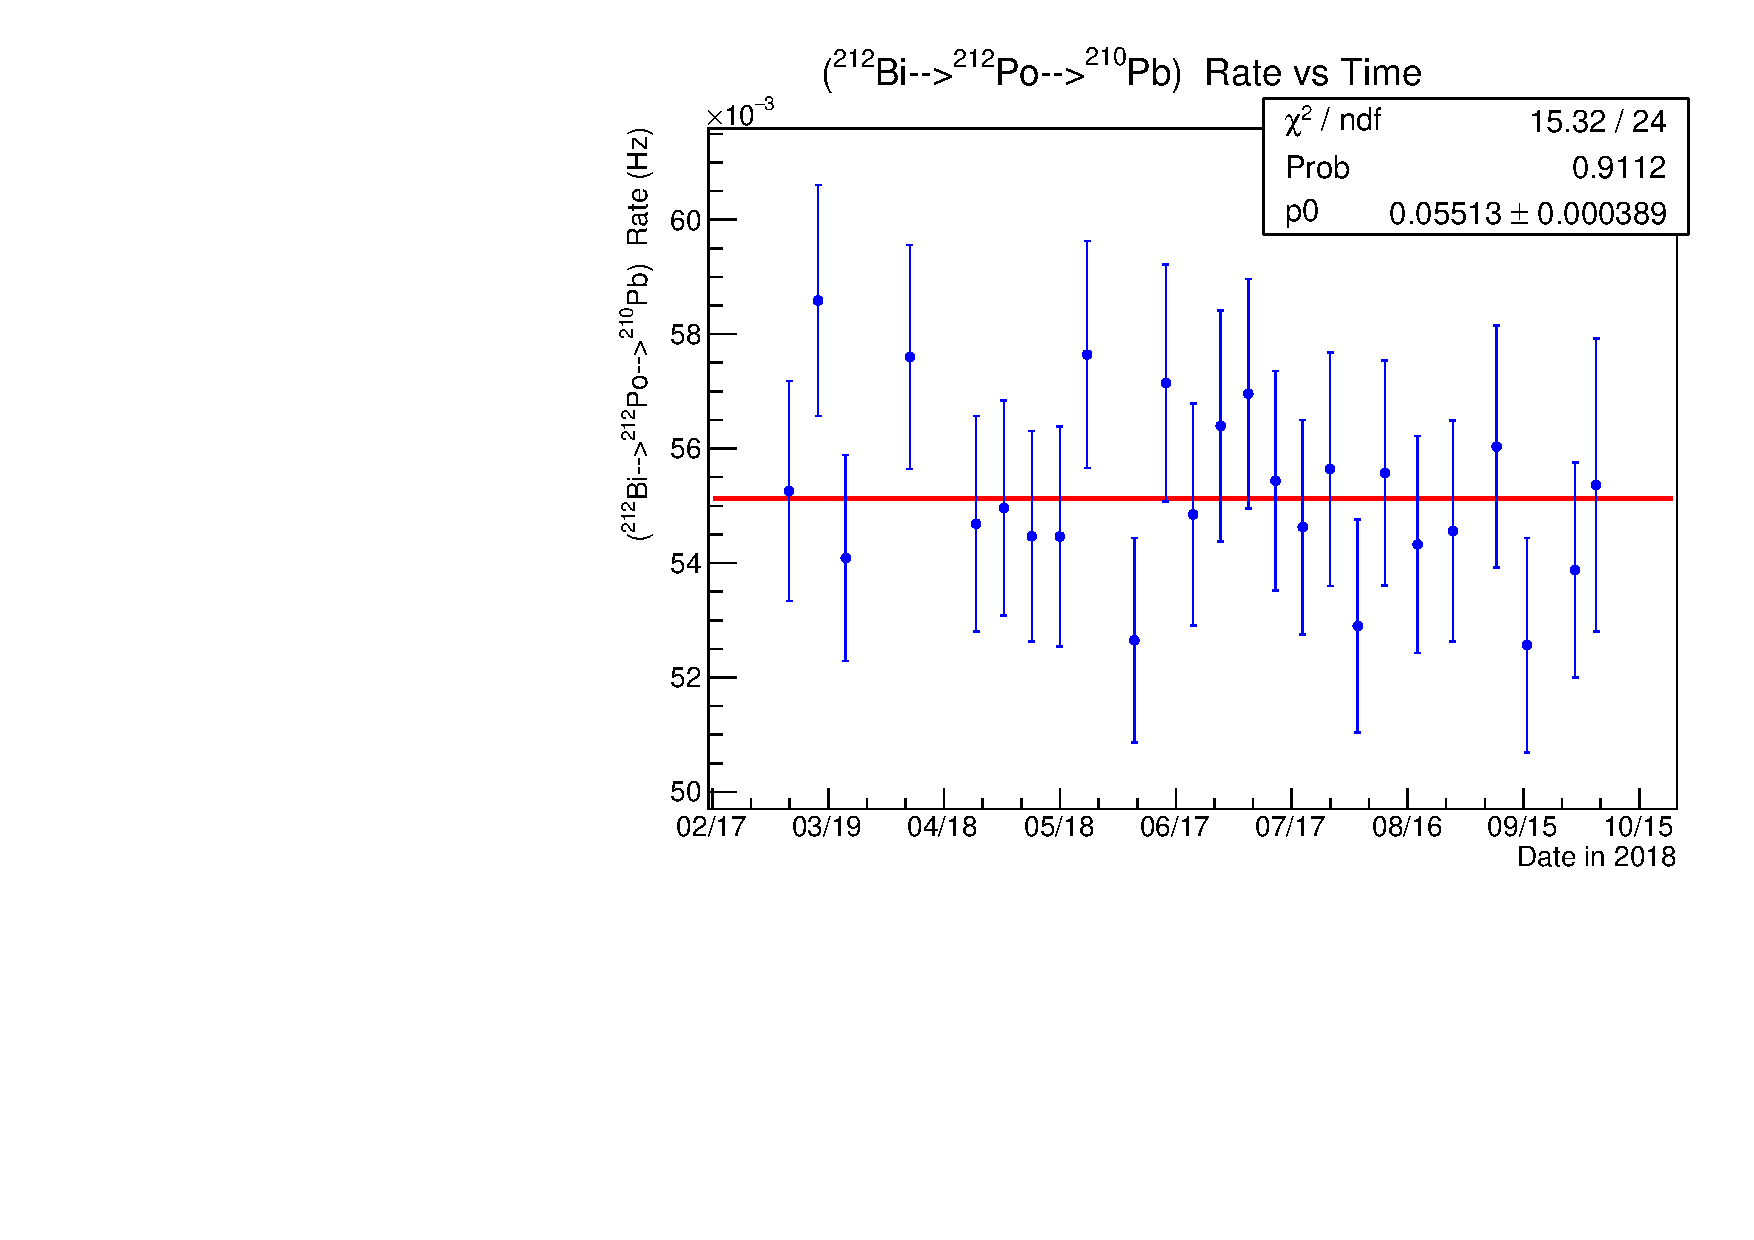
\includegraphics[width=0.9\textwidth]{figures/BiPo212RatevsT.pdf}
\caption{\label{fig:BiPo212RatevsT}Full AD BiPo-212 decay rate versus time. Shaded regions indicate periods where the reactor was on.}
\end{figure}

\begin{figure}[!h]
\centering
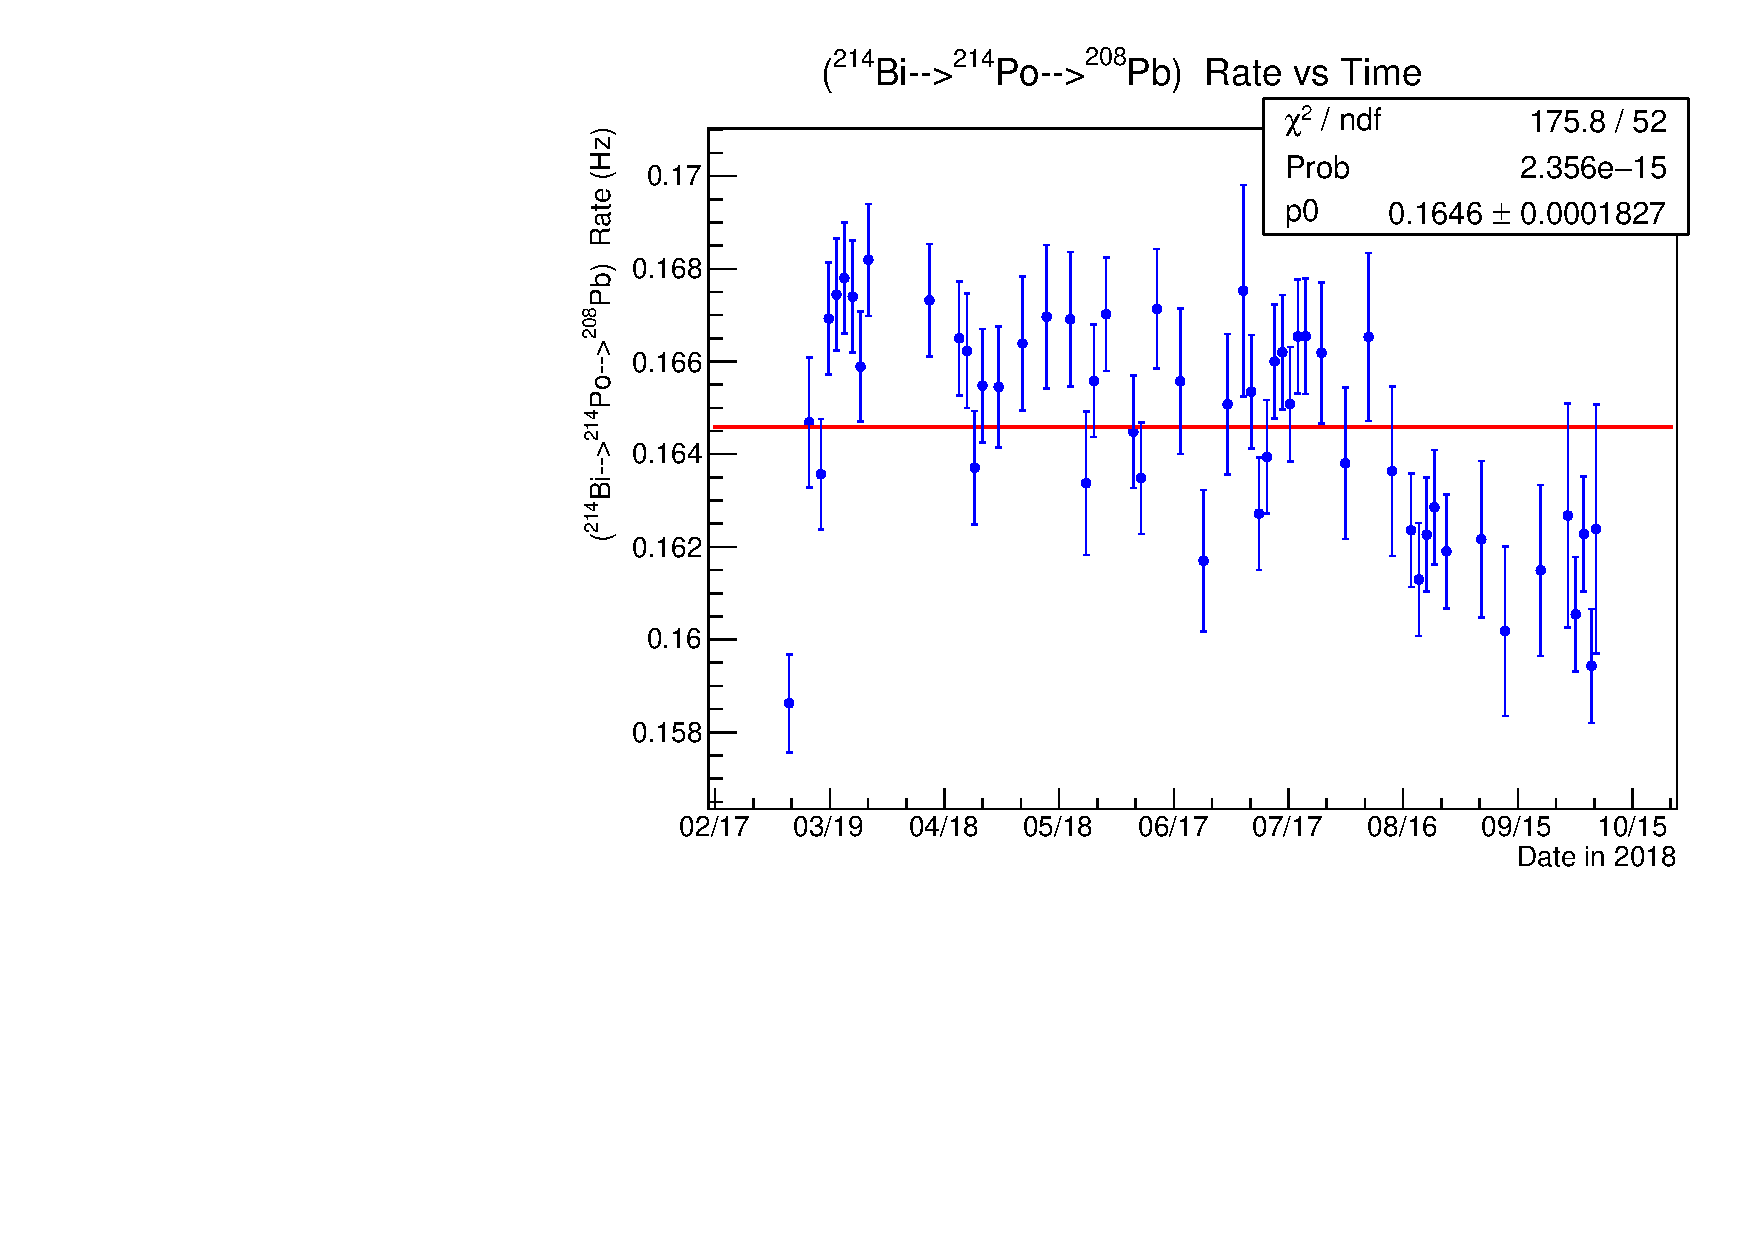
\includegraphics[width=0.9\textwidth]{figures/BiPo214RatevsT.pdf}
\caption{\label{fig:BiPo214RatevsT}Full AD BiPo-214 decay rate versus time. Shaded regions indicate periods where the reactor was on.}
\end{figure}

Since these decays are an IBD-like background, they need to be measured and leakage into our IBD selection quantified. In practice, given the high energy resolution of our detector ($\sim5\%/\sqrt{\textrm{MeV}}$), the alpha peaks from these events are well separated from the neutron capture peak near 0.53~MeV.

In principle, a uniformly dissolved source such as trace $^{232}$Th giving a signature decay sequence can be used to monitor relative cell volumes assuming that rate is proportional to volume. However, there is no guarantee given that we cannot be sure of where this trace material comes from, we also cannot be assured that it is uniformly distributed in our detector. Also, our low detection efficiency for the $^{212}$Bi$\rightarrow^{212}$Po decay combined with the already trace amount present in our detector gives a detection rate per cell of less than one decay per hour. A 1\% measure of relative cell volumes with this decay rate would require nearly 3 years of data.

This study focuses on using the nearly monoenergetic alphas from these decays to measure the stability of the energy calibration, PSD and the position and energy resolution of the AD. 

\subsection{Validation of data}
Before proceeding to use BiPos as a valid detector stability or calibration source we need to verify that we are seeing what we expect and that the data are not systematically suspect. Perhaps the primary validation comes from the expected time distributions. As previously mentioned, the lifetimes of the Polonium isotopes of interest are well known. We would not only expect to be able to find distributions consistent with these known lifetimes, but that different weightings and combinations of the data would give statistically consistent results. 

One of the issues particularly difficult in the Po-212 analysis is low statistics. When the data set is divided up into time bins or individual cells, the tail of the dt distribution (this distribution is used to calculate the rate and half-life) is sparsely populated. Since the fitter uses Chi-squared minimization and relies on Gaussian behavior, the low statistics bins can potentially bias the fits producing systematic effects in the results. In order to deal with this I reduced the number of bins in the distribution histograms and increased the integration time so that even the lowest statistic bin in the dt distribution would on average have a few tens of events. I also incorporated backgrounds into the model fitting so that my exponential fit includes a fixed background term and is not fit on the background subtracted data, thus increasing the statistics in the tail. The background is not allowed to float in the fit but is fixed from measuring the time displaced accidental window. 

The dt distribution for Bi-214/Po-214 ($dt=t_{\alpha}-t_{\beta}$) can be seen in Figure \ref{fig:Po214dtcum}. The accidental spectrum is produced from a far window with exactly the same cuts applied as for the expected prompt beta but extending forward in time from the delayed alpha from $10\tau$ to $46\tau$ where $\tau=2.37~\mu$s, the lifetime of Po-214. The accidental background is measured 12 times longer than the prompt signal to reduce statistical fluctuations. Figure \ref{fig:Po214dtcum} shows that an exponential decay with a lifetime of 164.1$\pm$0.4~$\mu$s fits the data well, in good agreement with the accepted value for the lifetime of 164.3$\pm$2.0~$\mu$s. 

If the data are binned by individual segment, we can check for systematic errors that are position dependent. Figure \ref{fig:Po214thalfvscell} shows the results of the same type of exponential fit analysis on a single segment basis.  
\begin{figure}[!h]
\centering
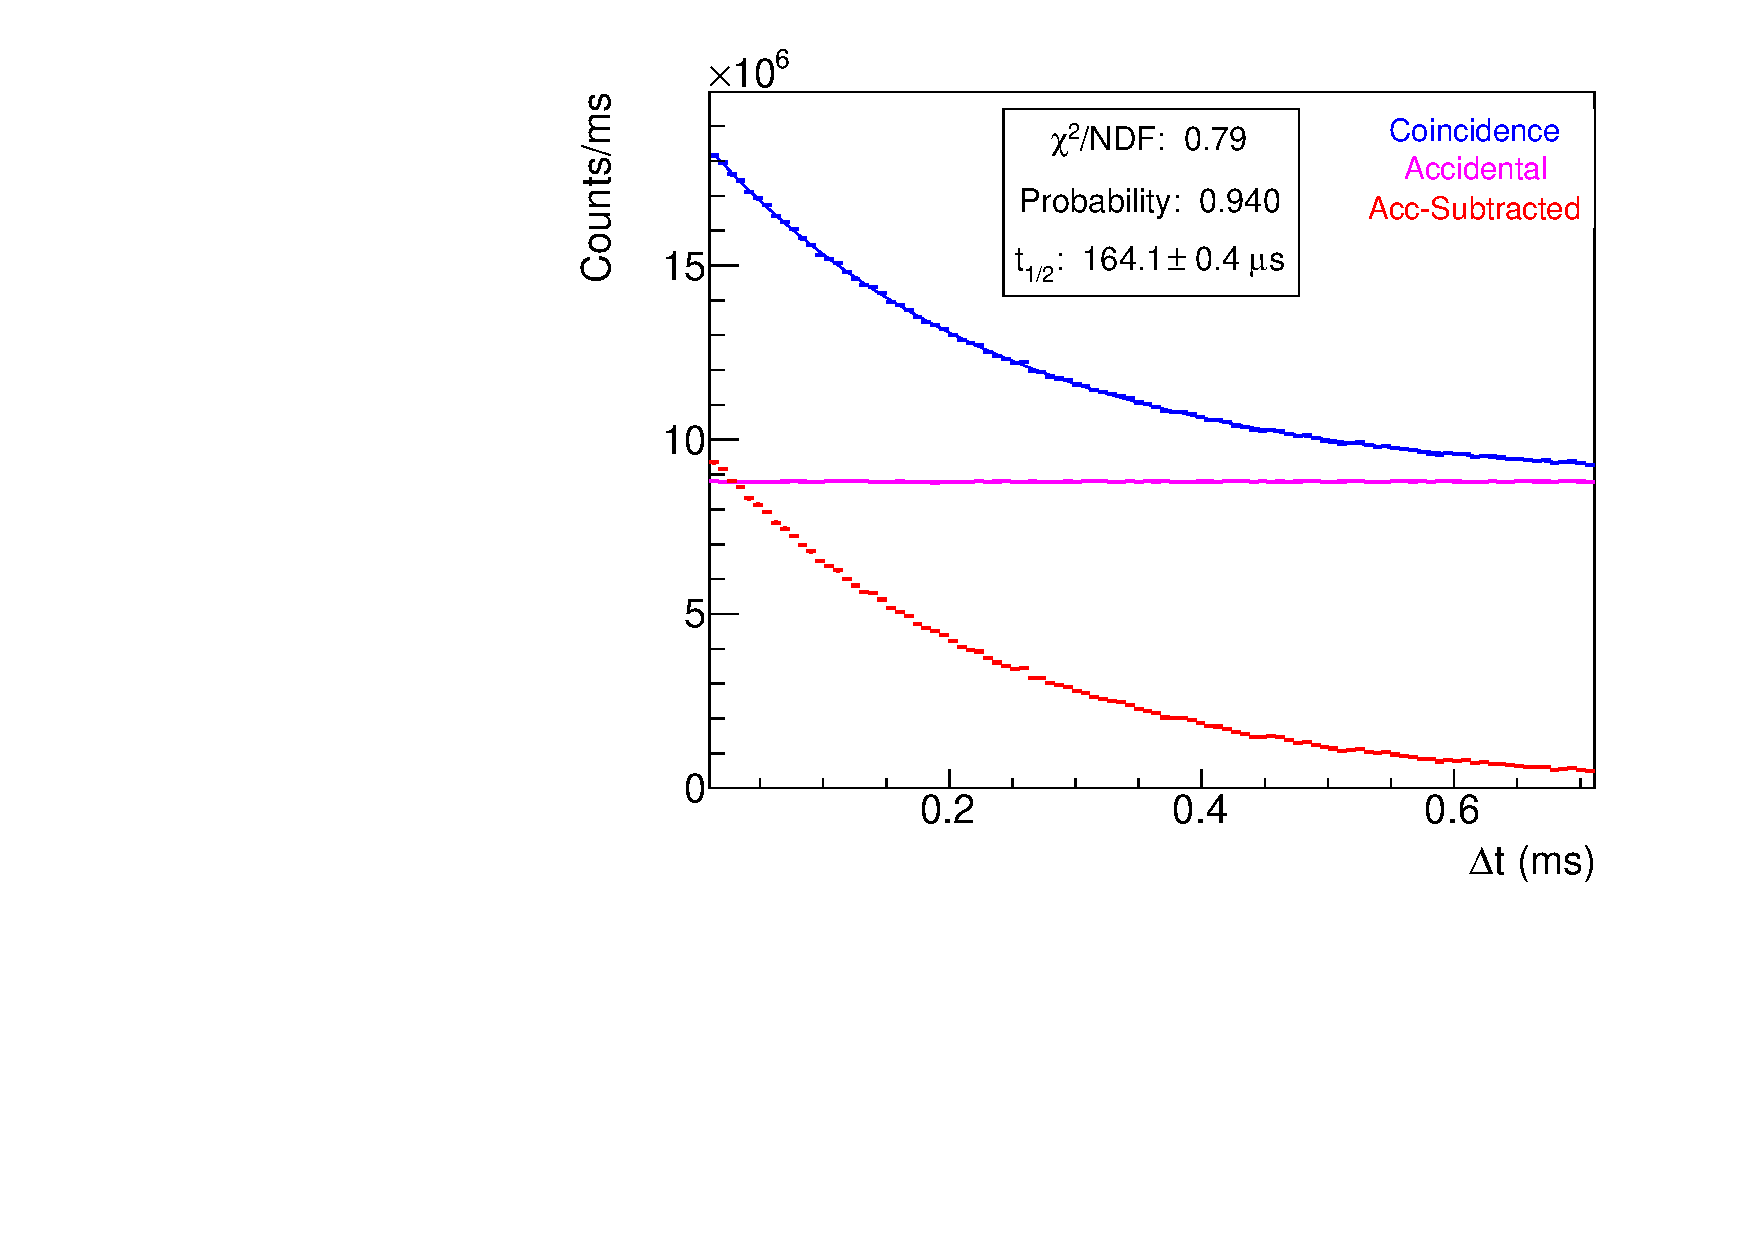
\includegraphics[width=0.7\textwidth]{../figures/BiPo214DeltaTSpectrum.pdf}
\caption{\label{fig:Po214dtcum}dt distribution for total PRD data set for Bi214/Po214. An exponential + background fit is performed on the full coincidence distribution (blue) where the background is fixed by the measured flat accidental distribution (magenta). }
\end{figure}

\begin{figure}[!h]
\centering
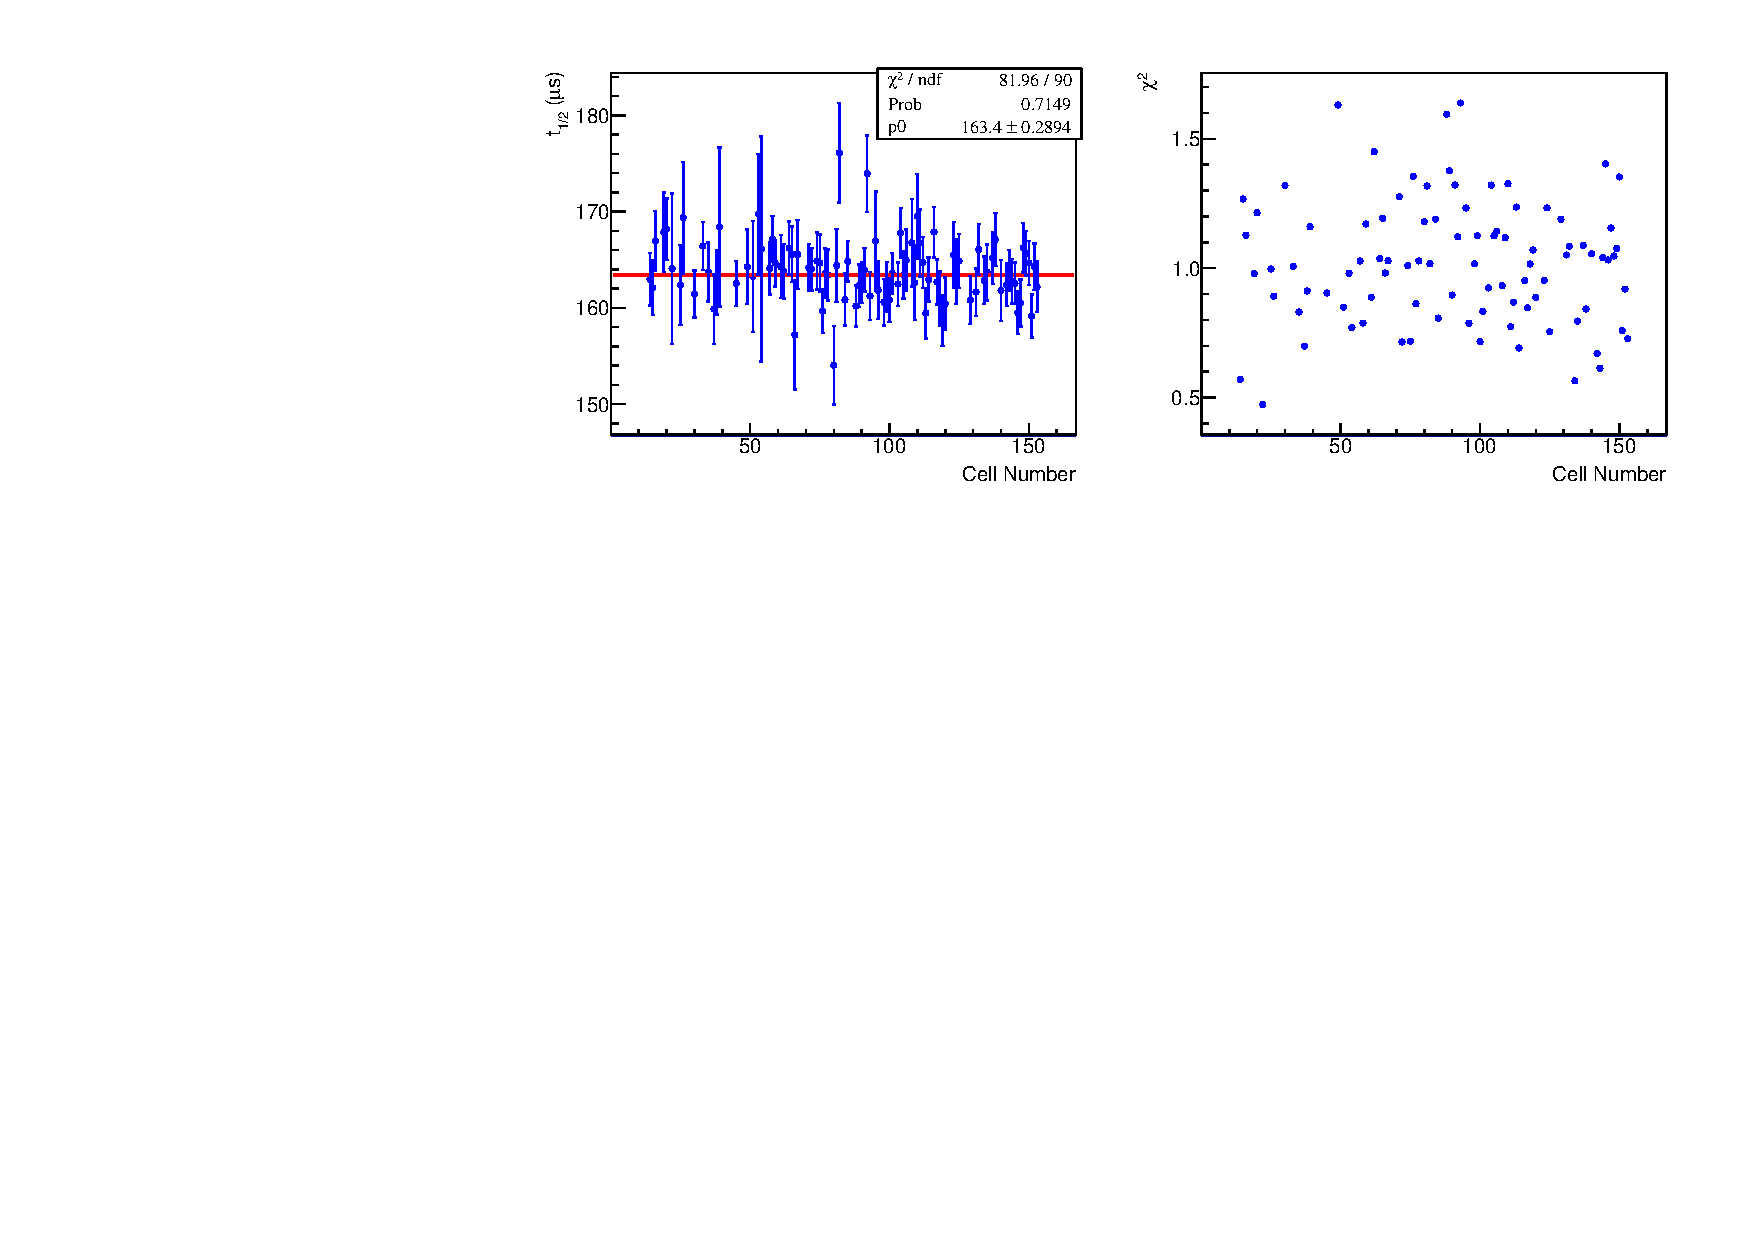
\includegraphics[width=0.96\textwidth]{../figures/BiPo214dTvsCell.pdf}
\caption{\label{fig:Po214thalfvscell}(Left)Half life versus segment (cell) for Bi214/Po214. (Right)$\chi^2$/NDF for the exponential fits for each cell demonstrating they are distributed fairly well about 1.}
\end{figure}

If the data are binned in time, we can check for systematic errors that are time dependent (for example, reactor on versus off differences). Figure \ref{fig:Po214thalfvstime} shows the results of the same type of exponential fit analysis binned in $\sim$48~hr time bins. The $\chi^2$/NDF is distributed about 1. The three analyses of the same data sets (single cumulative exponential distribution, error weighted average of exponential for each cell and error weighted average of exponential for each 48 hours of data) using different binning schemes and weights all yield results giving the same half life to within 0.7~$\mu$s each with a reasonable $\chi^2$/NDF. The difference between half-life versus time and half life from the cumulative dt distribution (Figures \ref{fig:Po214dtcum} and \ref{fig:Po214thalfvstime}) appears to be in slight tension statistically with what one might expect from the increase in statistical uncertainty arising from the non-optimal weighting in Figure \ref{fig:Po214dtcum}\footnote{The square root of the difference of the squares of the errors provides an estimate of the variation one might expect: $\sqrt{0.37^2-0.29^2}=0.23~\mu$s}. The difference between the half-life versus cell and the half-life from the cumulative dt distribution are in slight tension (at the 3$\sigma$ level using the difference of the squares of the errors as an estimate of $\sigma^2$) even though each appears statistically consistent on its own. This small tension is not likely to bias the energy stability analysis. It would have to be factored in when estimating the error on cell to cell rates since the rates are calculated from the half-life distributions, but since the Po-214 rates are not expected to be uniform from cell to cell, this analysis is not used in any detector validation study. These analyses point to a measured value for the half-life of Po-214 with a conservative uncertainty of $t_{1/2}(\textrm{Po-214})=164\pm1~\mu$s in good agreement with the accepted value but with half the uncertainty.  

\begin{figure}[!h]
\centering
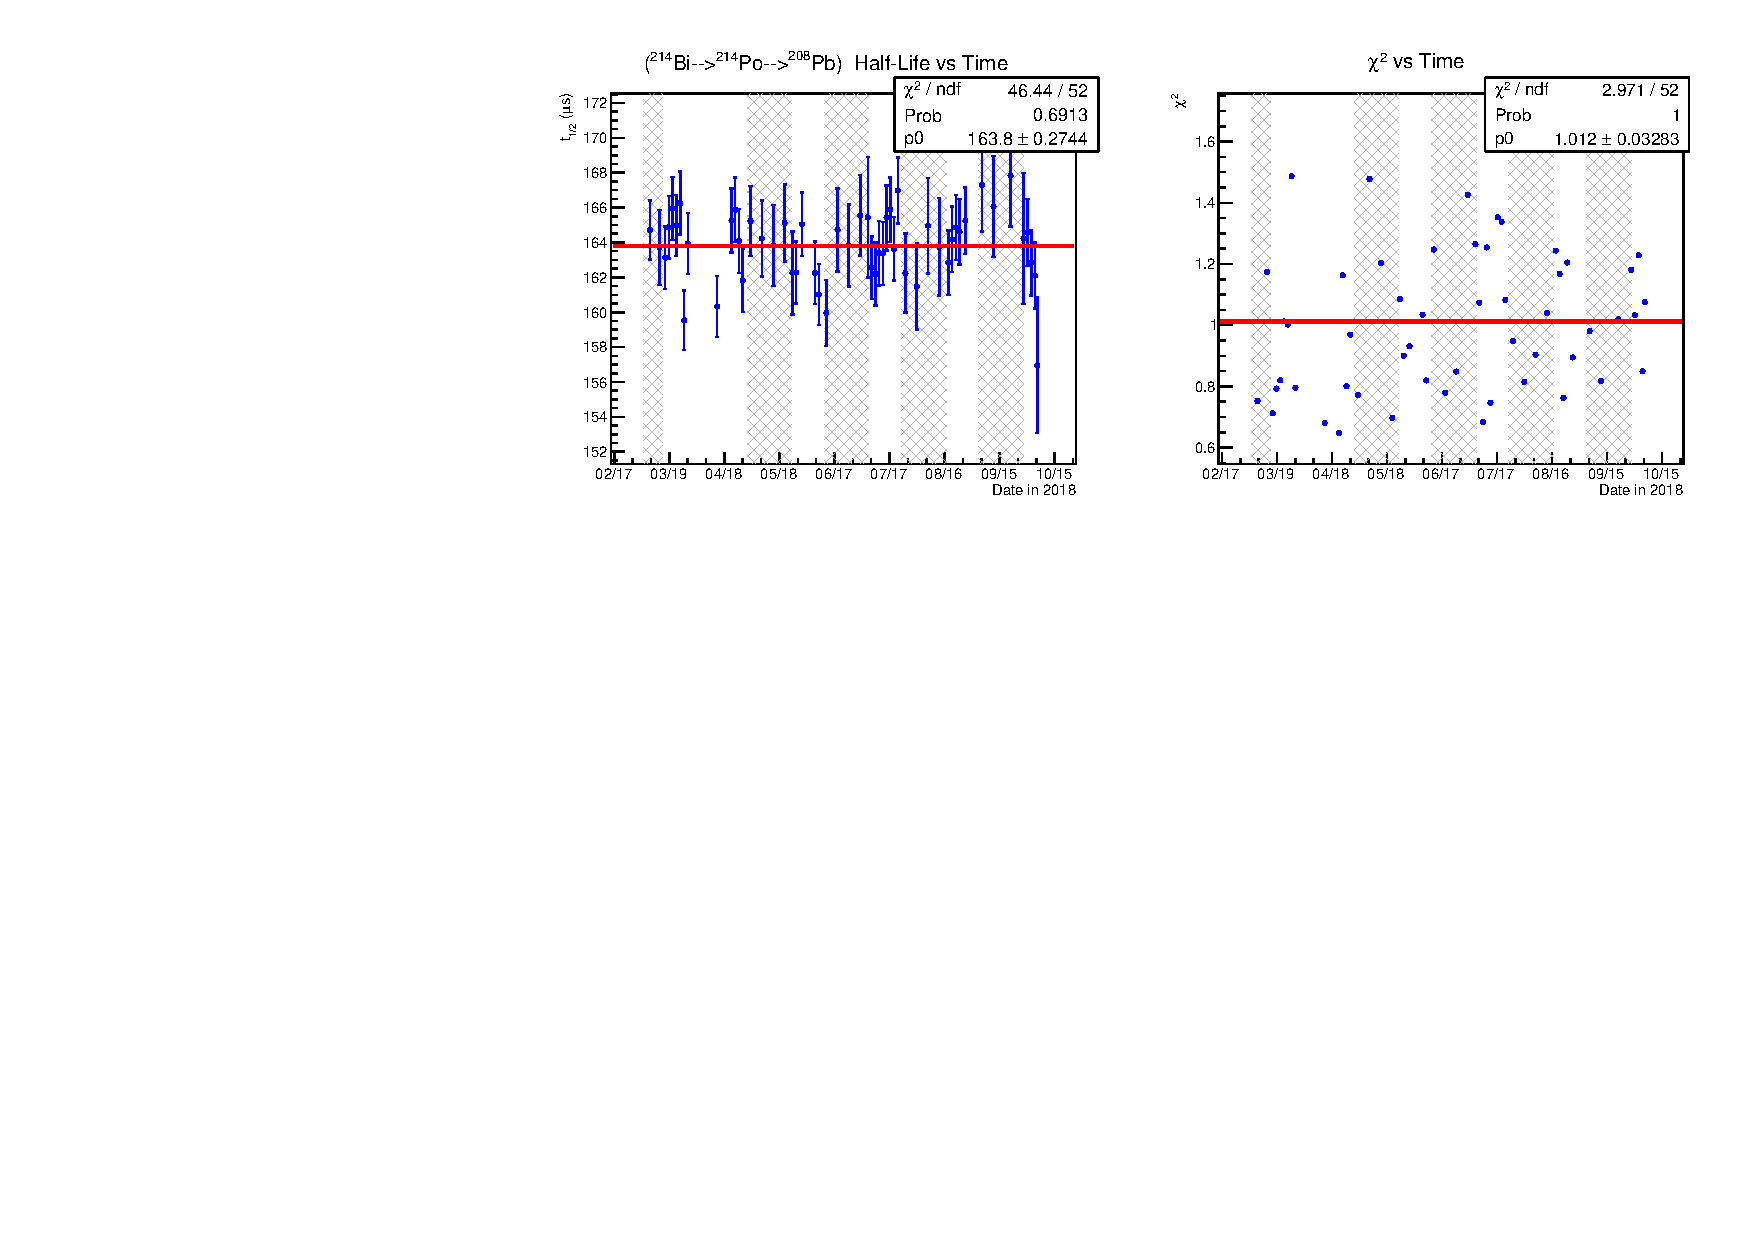
\includegraphics[width=0.96\textwidth]{../figures/BiPo214dTvsT.pdf}
\caption{\label{fig:Po214thalfvstime}(Left)Half life versus segment (cell) for Bi214/Po214. (Right)$\chi^2$/NDF for the exponential fits for each cell demonstrating they are distributed fairly well about 1.}
\end{figure}

The analysis of Po-212 is not as straightforward. With an accepted half-life of $299\pm2$~ns this isotope is difficult to measure even with a continuous buffering ADC. The PMT signals in our detector vary in length but can be as much as a few hundred nanoseconds long. Although the recorded waveforms are restricted to a maximum length of 596~ns, data indicates that two or more events can only be reliably reconstructed with proper energy and PSD if they are sufficiently separated in time. Earlier studies showed that after about 650~ns the reconstruction is valid\footnote{See Figure 31 of https://docdb.wlab.yale.edu/prospect/ShowDocument?docid=2377}. I have imposed a software veto of 700~ns between successive pulses, thus losing $>$80\% of the Po-212 signal. Analysis shows that we have a total detector rate of about 55 mHz of which we accept about 10 mHz. This small signal means that we have to be careful not to introduce bias by low statistics bins at the edges of the energy, PSD, dZ and dt plots. For this reason I increased the time bins from 48 hr for the Po-214 to 7 days for the Po-212 analysis. 

Given that the PSD of the Po-212 and Po-214 signals are essentially identical, they are only discriminated based on the energy and timing. The energy cut on the alpha peak used for the Po-212 is $E>0.95$~MeV or about 2.2~$\sigma$ above the mean energy of 0.845~MeV for the Po-214 peak. Thus we would expect some leakage (about 1.4\% of the Po-214 events should be above 0.95~MeV) of Po-214 into the Po-212 data set. Of course, only a small fraction of these will pass the timing cuts, but nonetheless, this represents a small additional background on top of the truly accidental background. 

The way the analysis works is to first identify the delayed alpha since those events are rarest and most cleanly identifiable. Then a reverse (earlier) time search is done for the prompt beta event. The accidental background is measured in a window located in the time forward (later time) direction from the delayed alpha. Because the accidental background is determined from a window located later in time from the delayed event, the small correlated background from Po-214 events will not be included in the accidental background subtraction. In order to account for this, the beta signal in a window from 5~$\mu$s to 711~$\mu$s (3 Po-214 lifetimes) backward (earlier) in time from the delayed alpha  was measured in addition to the accidental rate in the time forward window. The 5~$\mu$s ensures no Po-212 signal remains. This earlier time window was then fit using the expression $f=[A]\exp{(-t/\tau_{214})}+B$ where $\tau_{214}$ was the accepted lifetime for Po-214 of 0.1643/log(2)~ms and $B$ was fixed to the constant accidental background rate from the time forward (later in time) window. These background terms were then inserted as fixed terms into the full dt distribution fit using the following expression:
\begin{equation}
f=[C]\exp{(-t/[\tau])}+A\exp{(-t/\tau_{214})}+B,
\label{eqn:fdecay}
\end{equation}
where only the bracketed parameters are free in the fit. This procedure is followed for all dt distributions: binned by time or segment or the cumulative distribution. Figure \ref{fig:Po212dtplusbkg} shows the cumulative dt distribution and the background model included in the fit. The small non-statistical fluctuations in the background model contributing to the low probability of the fit are not worrisome, given the size of the background relative to the Po-212 signal. The Po-212 distribution fit yields a half-life of $t_{1/2}(212)=296.6\pm1.4$~ns in decent agreement with the accepted value of $299\pm2$~ns.  The probability of the Po-212 distribution fit is about 39\% which appears acceptable if we looked no further, but closer examination indicates there is tension in the model. Figure \ref{fig:Po212halflifevsfitrange} shows the half-life fit as a function of the number of half-lives included in the fit. Note that the window for dt begins at $dt=0.7~\mu\textrm{s}\approx2.3t_{1/2}^{(212)}$. We can see that the half-life appears to exhibit a non-statistical dependence on the length of the dt window included, beginning at a half-life of 301~ns for $dt\approx3.7t_{1/2}^{(212)}$ and decreasing to a minimum half-life of $<293$~ns for $dt\approx4.5t_{1/2}^{(212)}$. The difference between these two points is in tension at a level of $>2\sigma$. This degree of variation in half-life especially from 2.3 to 4.5 half-lives appears to be in tension from a purely statistical standpoint pointing to a possible systematic issue in the data. However, after weeks of effort, I was not able to uncover any source of this systematic effect. As the dt window is increased in length, eventually the Po-212 signal fades out and the residual Po-214 plus accidental background dominates the fit. It is not surprising that when the distribution is dominated by a region that is depleted of Po-212 signal that the fit for the Po-212 life time is not good statistically. Essentially the fit is working to minimize statistical deviations in the Po-212 depleted region at the expense of finding a good fit in the non-depleted region. Although the background is relatively small in this analysis due to the short duration of the prompt window, still above 9 half-lives the Po-212 signal is less than the small background. Furthermore, large variations in the fit probability can be seen to arise from simply changing the bin width and thus the number of bins in the fixed fit region from $0.7~\mu s<dt<1.7~\mu s$ as can be see in Figure \ref{fig:Po212halflifevsNbinsX}. Depending on the number of bins chosen one could get a probability of 0.6 or 0 using exactly the same data set, suggesting a non-statistical effect that either cancels or gets exaggerated with certain bin width choices. The half-life value is not very sensitive to bin width. 
\begin{figure}[!ht]
\centering
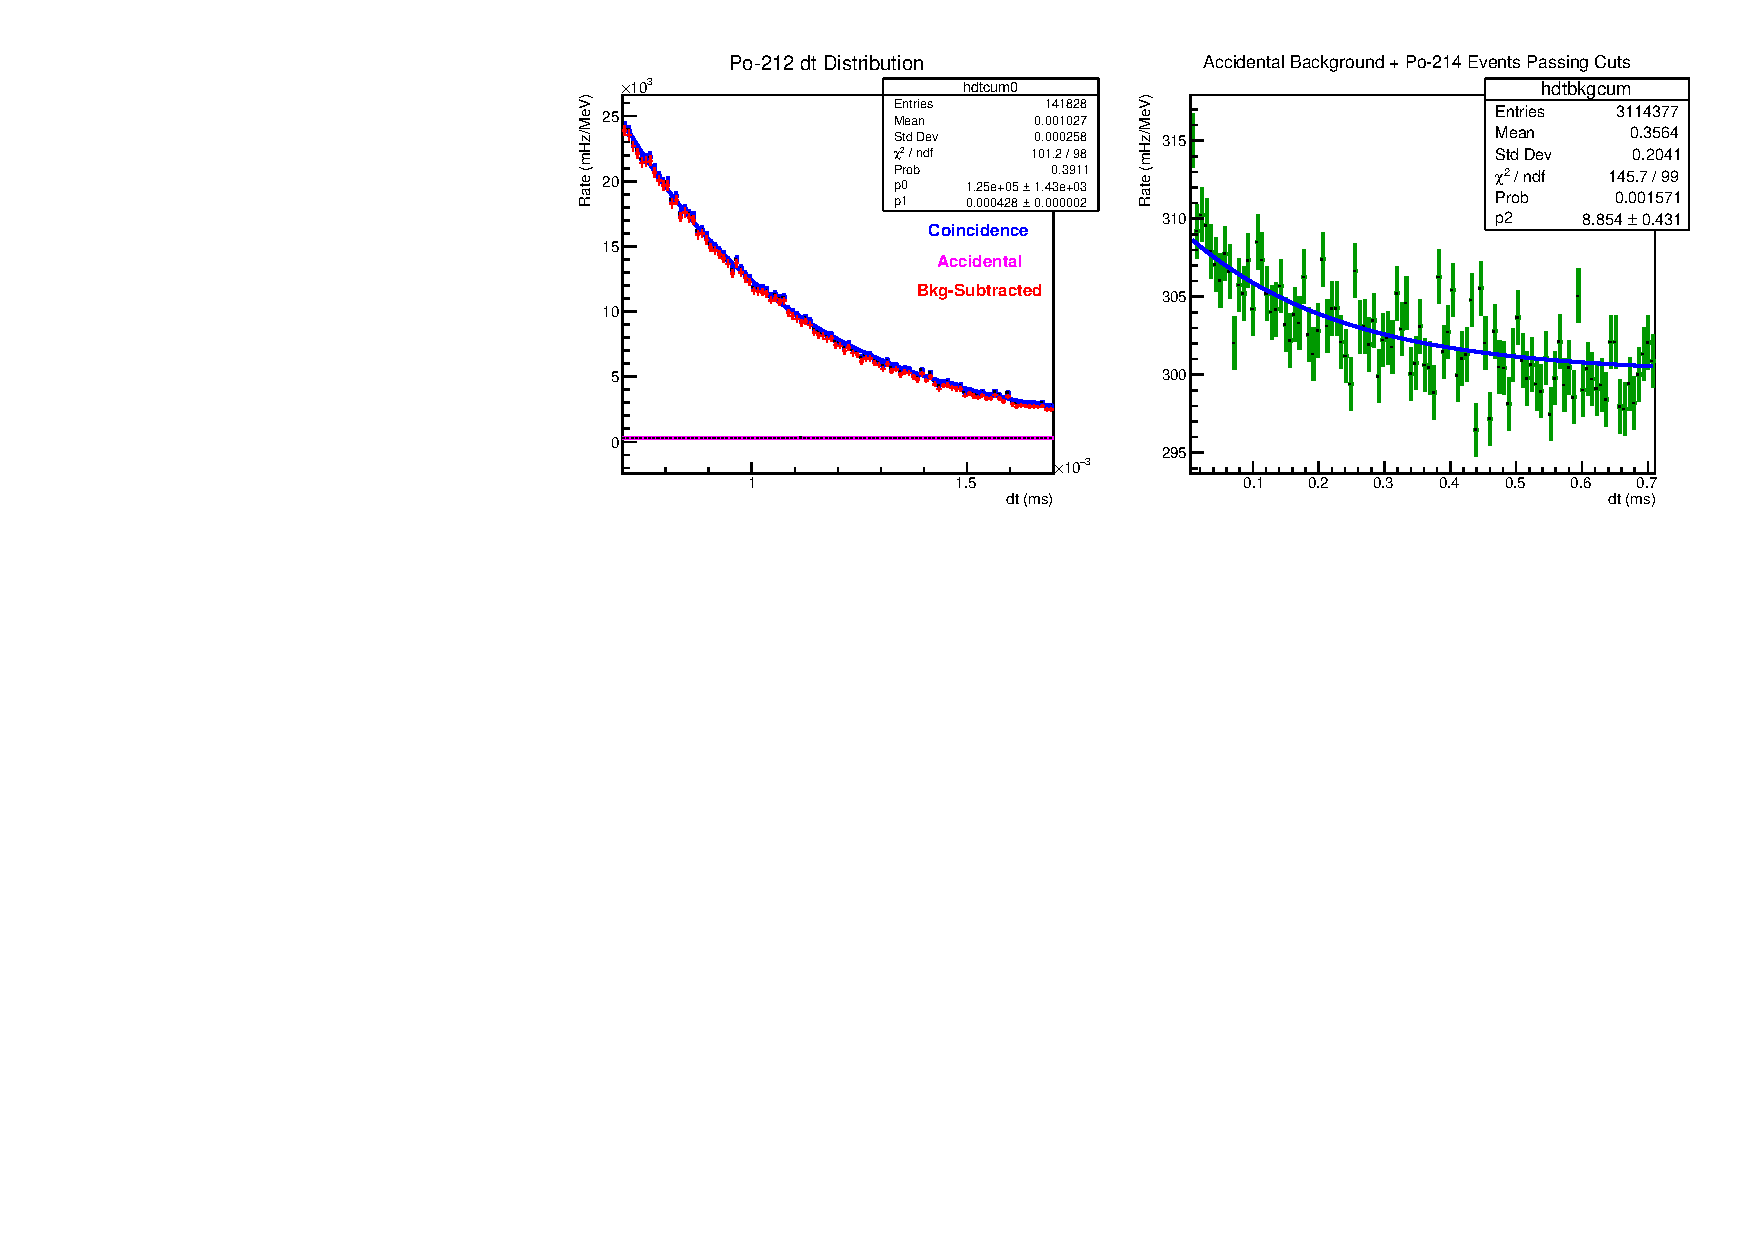
\includegraphics[width=0.96\textwidth]{../figures/Po212dtPlusBkg.pdf}
\caption{\label{fig:Po212dtplusbkg}(Left)Alpha minus beta dt distribution for Po-212. (Right)Background of Po-212 dt distribution measured from 5~$\mu$s to 711~$\mu$s after the delayed alpha fit to a constant plus exponential where the constant is fixed from the accidental window and the time constant is the lifetime of Po-214.}
\end{figure}

%make plot using script BiPodtFitRange.C
\begin{figure}[!h]
\centering
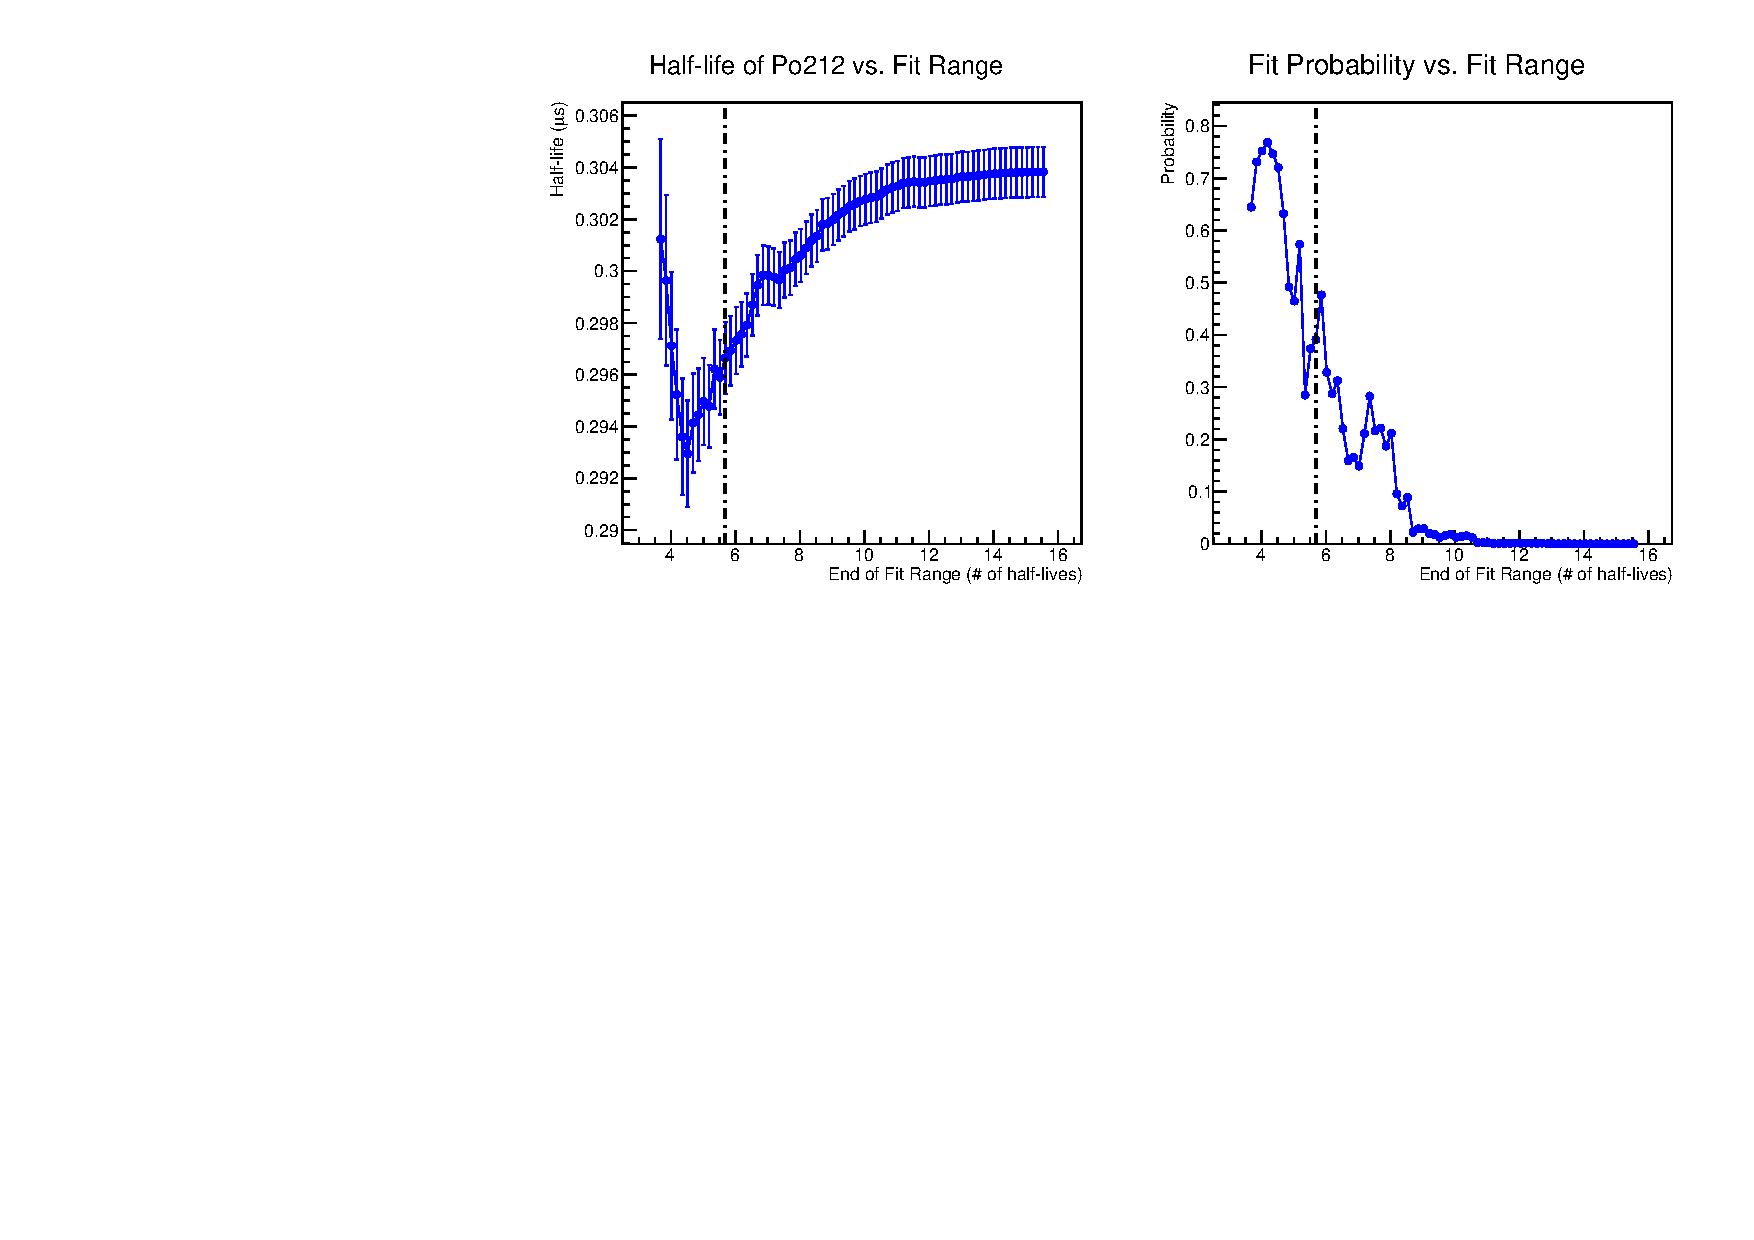
\includegraphics[width=0.96\textwidth]{../figures/Po212HalfLifevsFitRange.pdf}
\caption{\label{fig:Po212halflifevsfitrange} (Left)Half-life of Po-212 from fit versus the end point of the dt distribution fit range. Black vertical line shows end point used in analysis. (Right) Fit probability versus end point of the dt distribution fit range.}
\end{figure}

%make plot using script BiPodtFitRange.C
\begin{figure}[t]
\centering
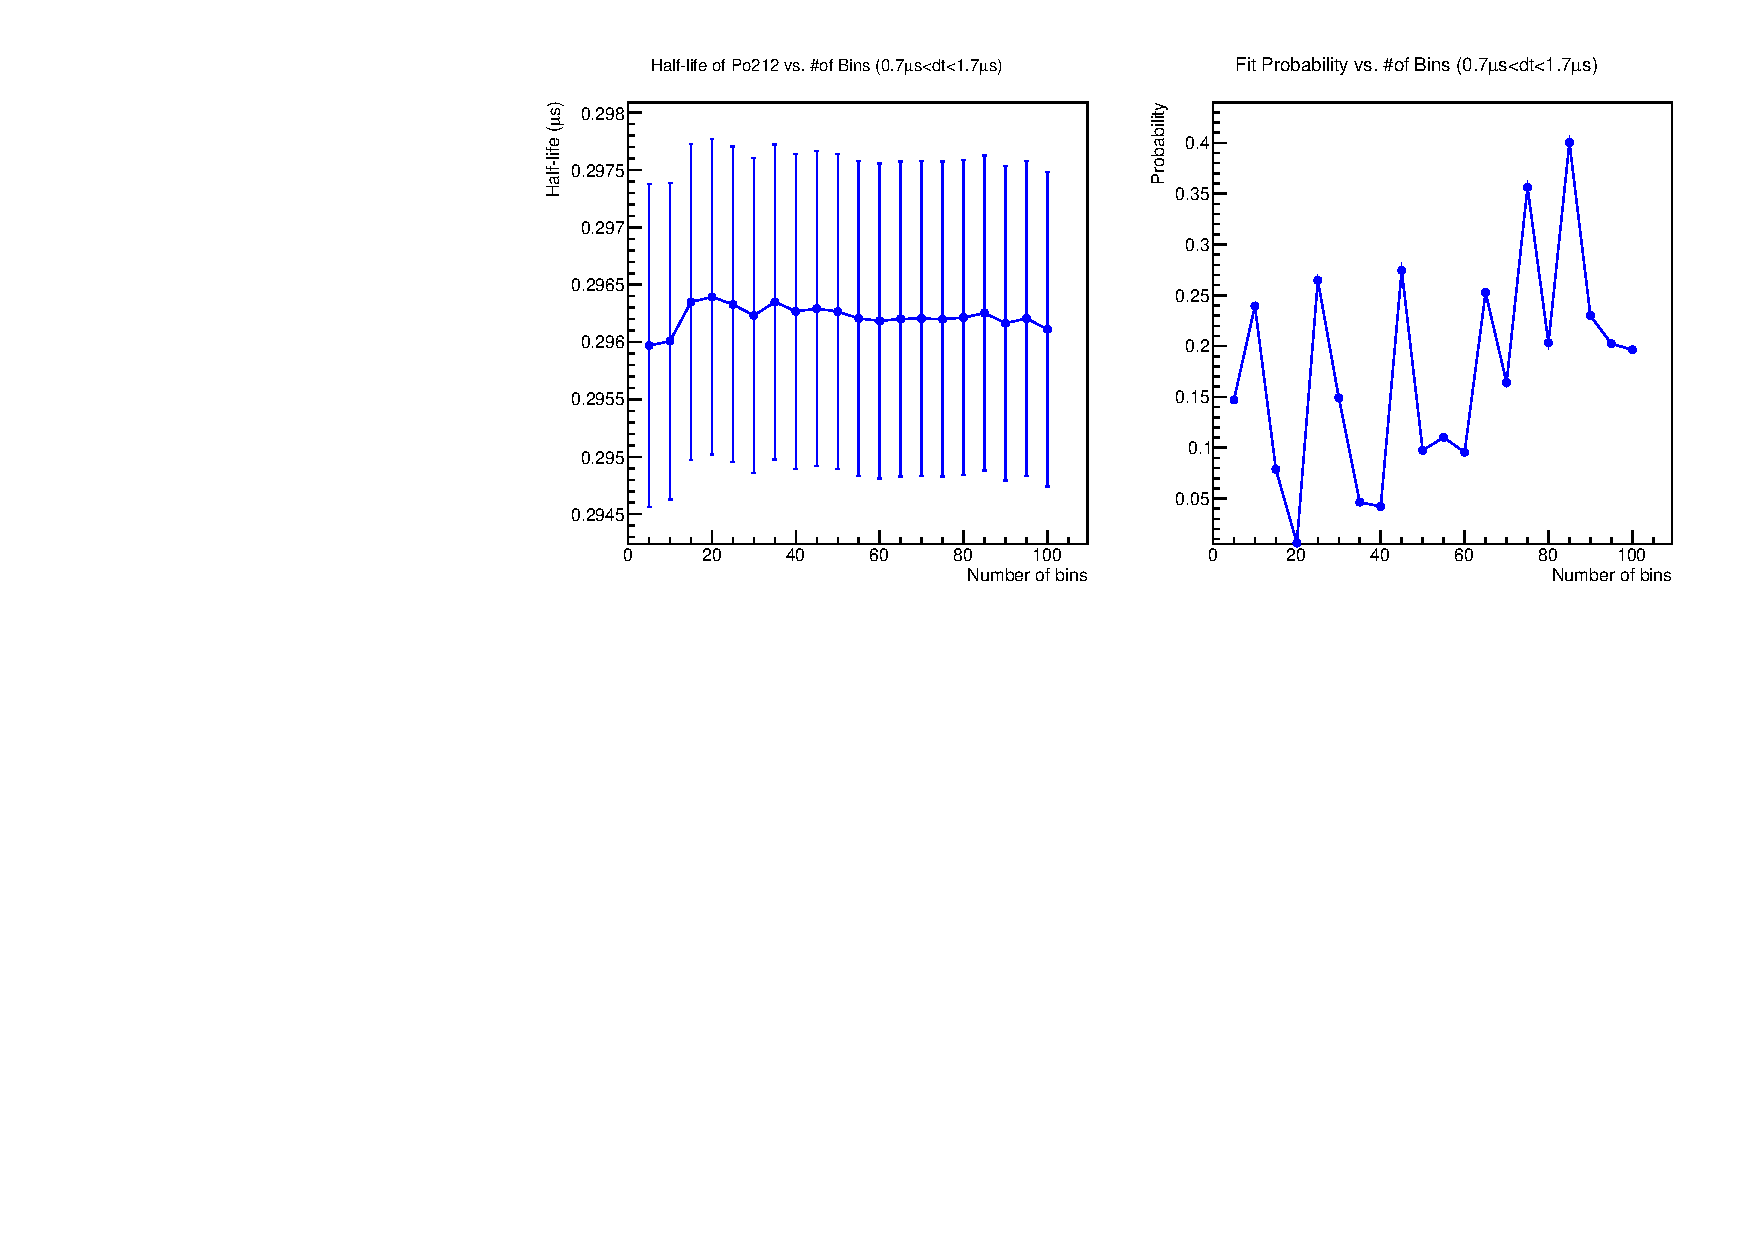
\includegraphics[width=0.96\textwidth]{../figures/Po212HalfLifevsNbinsX.pdf}
\caption{\label{fig:Po212halflifevsNbinsX}(Left)Half-life of Po-212 from fit versus the number of bins in the fixed fit range. Variation in the half-life from the fit is much less than 1$\sigma$.  (Right) Fit probability versus number of bins in the fixed fit range.}
\end{figure}

Given that the time distribution is used to provide the BiPo rates, one might ask the degree to which a systematic effect like this would affect the rate analysis and whether or not it could be trusted. Figure \ref{fig:Po212RatevsNbinsXandFitRange} shows the variation in the rate from changing the end point of the fit and the bin width in the fixed fit range. Starting with the Po-212 term in the exponential fit ($Ae^{-x/\tau}$), the rate is given by $R=A\tau$. One can see that using the data range chosen for this analysis (see vertical black line in Figure \ref{fig:Po212RatevsNbinsXandFitRange}) an additional point to point $\pm1$\% systematic error should be assigned to any rate analysis for this systematic effect. 
%make plot using script BiPodtFitRange.C
\begin{figure}[t]
 	\centering
 	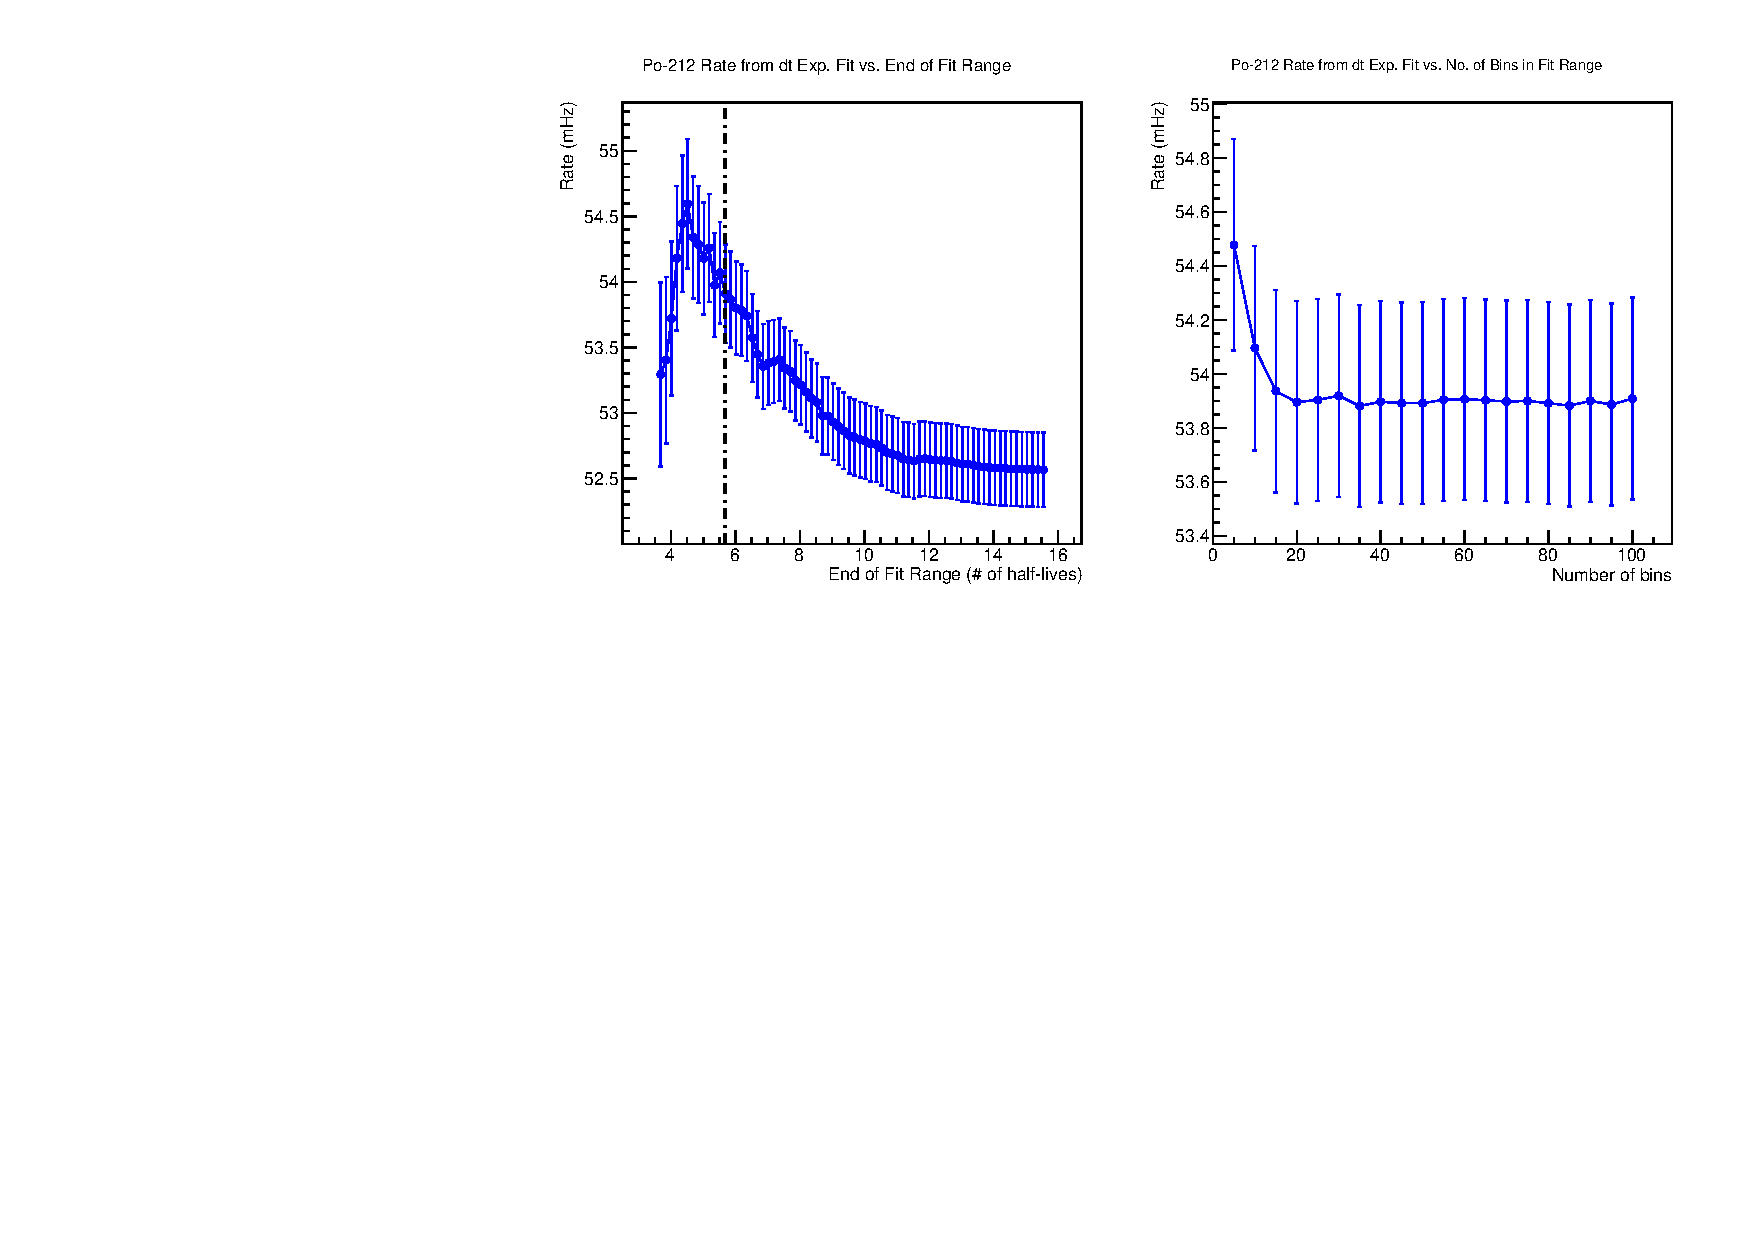
\includegraphics[width=0.96\textwidth]{../figures/Po212RatevsNbinsXandFitRange.pdf}
 	\caption{\label{fig:Po212RatevsNbinsXandFitRange}(Left)Po-212 rate from fit versus the end point of the fit range. Variation in the rate from the fit is much less than 1$\sigma$.  (Right) Po-212 rate from fit versus the bin width in the fixed fit range. Variation in the rate from the fit is much less than 1$\sigma$.}
\end{figure}

The obvious question is how the end point and number of bins was chosen. When subdividing the data in time, there is freedom in choosing the integration length which I chose to be $\sim$7 days to avoid low statistics issues. However, there is no such freedom for the individual segment analysis. For the Po-212 analysis I selected an endpoint for the dt distribution of 1.7~$\mu$s and 15 bins over the range of dt from 0.7~$\mu$s to 1.7~$\mu$s. Given the cuts that have been utilized (see Section \ref{sec:cuts}), this is expected to give on average a population of 27, 32 and 37 events in the 3 lowest statistics bins (bins 15, 14, and 13 respectively) of the dt distribution, which is expected to be sufficient statistics to not significantly bias the data. Figure \ref{fig:Po212thalfvscell} shows a comparison of the half-life cell to cell. The cell to cell half-life fit to a constant gives a half-life of $291.8\pm1.4$(stat)~ns has a decent probability of 0.22, upholding the expectation that the data are not significantly biased but are in tension with the accepted value of $299\pm2$~ns\footnote{As noted in the following publication, there are difficulties with measuring the half-life of this isotope which become obvious in the spread of the measurements relative to their quoted errors: https://arxiv.org/abs/1812.10997. They measure a half-life of $294.8\pm1.9$~ns. Happy reading Ukranian!}. However, when the bin size is halved (i.e. 30 bins are used instead of 15), the probability of the constant fit reduces to 0.08 and the half-life goes to $288.1\pm1.3$~ns far from the accepted value, suggesting bias has entered the analysis. The error on the fit is reduced marginally from 1.36~ns using 15 bins to 1.33~ns with 30. The reduction in half-life, uncertainty and probability with only a change in binning of the data, points to the low energy bins being biased towards lower values. This makes sense intuitively since the $\sqrt{N}$ statistics assumed by the fit are not symmetric about the mean value of $N$ for small $N$ but give lower error for $N-\sigma$ than for $N+\sigma$. Using the same bin width and dt fit range in the time dependent analysis with approximately 1 week of data per point gives about 100 events in the lowest statistics bin which is not expected to create significant bias. 

 Figures \ref{fig:BiPo212Rate} and \ref{fig:BiPo214Rate} show the rate in the AD as a function of time.

A full discussion of cuts can be found in Section \ref{sec:cuts}.
\begin{figure}[!h]
	\centering
	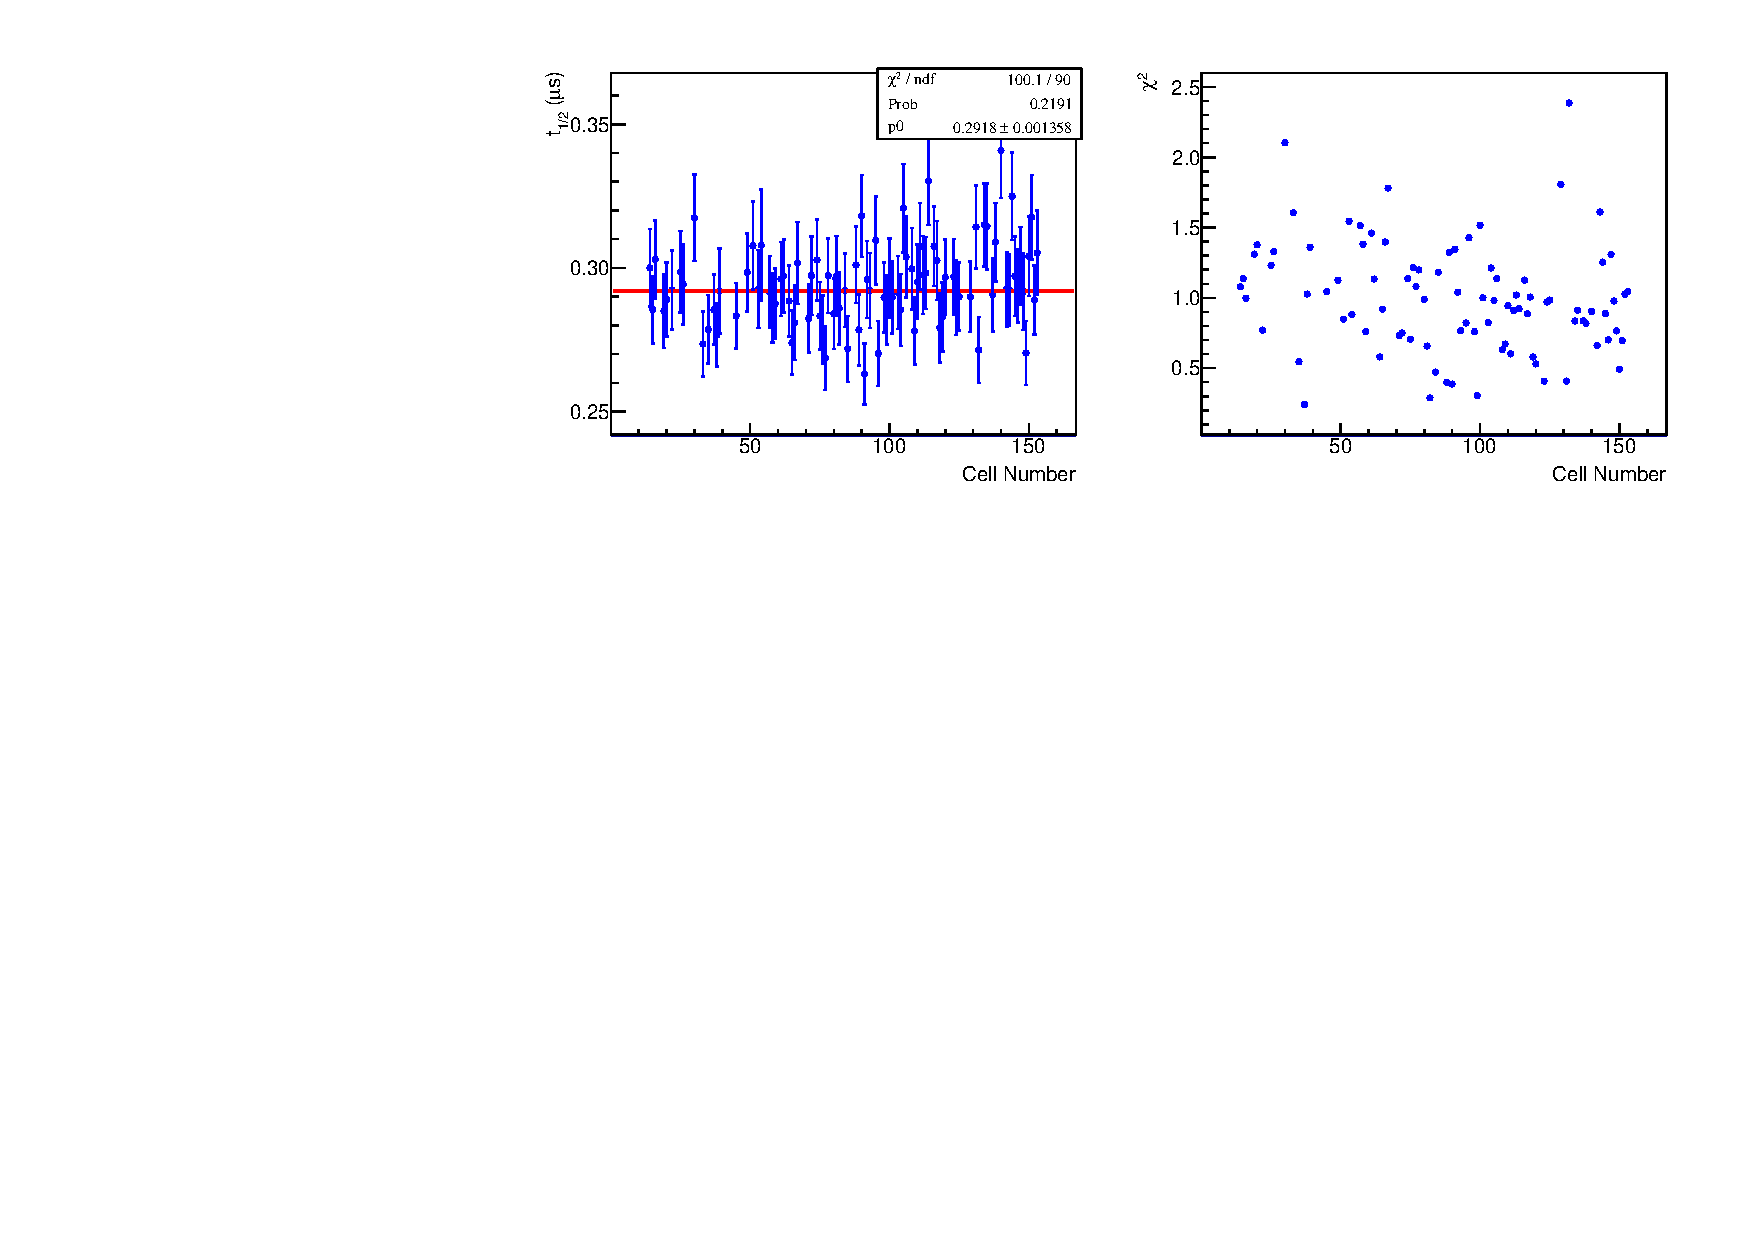
\includegraphics[width=0.96\textwidth]{../figures/BiPo212dTvsCell.pdf}
	\caption{\label{fig:Po212thalfvscell}(Left)Half life versus segment (cell) for Bi212/Po212. (Right)$\chi^2$/NDF for the exponential fits for each cell demonstrating they are distributed fairly well about 1.}
\end{figure}

\subsection{Plots details}
The following list of plots will be made for both the decays of $^{214}\textrm{Bi}\rightarrow$$^{214}\textrm{Po}\rightarrow$$^{210}\textrm{Pb}$ and $^{212}\textrm{Bi}\rightarrow$$^{212}\textrm{Po}\rightarrow$$^{208}\textrm{Pb}$. Any plots involving alpha energy will be shown in reconstructed energy and ``smeared" reconstructed energy. Smeared reconstructed energy is an attempt to give all cells of the detector nearly the same energy resolution constant over time. The energy resolution is not identical segment to segment and is also degrading nearly linearly with time. Smeared energy adds a random noise that is segment and time dependent intended to produce a uniform energy resolution across all cells that does not change much with time. The energy resolution of the worst cells towards the end of the given analysis period then set the resolution of the full detector. For this analysis pass 2019B, the target resolution was 325 PE/MeV or approximately 5.5\% at 1 MeV. Beta energy is not smeared in these plots since betas are not used in the stability plots for this analysis.
\begin{enumerate}
\item{Alpha mean energy and smeared energy vs. segment. }
\item{Width (1$\sigma$) of the alpha energy distribution and the smeared alpha energy distribution vs. segment. }
\item{Width (1$\sigma$) of the $\Delta$Z distribution, separation distance between the alpha and beta vs. segment. This is a measure of the position resolution. }
\item{RMS width of the Z-position distribution of alphas vs. segment. }
\item{Mean of the Z-position distribution of alphas vs. segment. This will be a verification that the position reconstruction is working as expected and should be statistically distributed around zero.}
\item{Alpha mean energy and smeared alpha mean energy versus time. Ideally, this should be statistically consistent with a constant.}
\item{Alpha mean energy width and smeared alpha mean energy width versus time. This will track detector light yield and transport.}
\item{RMS width of the Z-distribution of alphas averaged across detector versus time. This shows the stability of the position reconstruction over time.}
\item{Width of $\Delta$Z distribution averaged across detector versus time. This tracks the position resolution over time.}
\item{Mean of the Z-position distribution of alphas vs. time. This will be a verification that the position reconstruction is working as expected and should be statistically distributed around zero.}
\item{Alpha energy and smeared alpha energy distribution for whole detector. This will be used to estimate leakage into IBD event selection.}
\item{Beta energy spectrum for whole detector. For Bi-214 the shape and endpoint is compared with a simulated spectrum to verify that the simulation properly captures the detector performance. Also, for Bi-214 the beta spectrum for segment 76 is provided. }
\item{Whole detector Po alpha Z-position distribution.}
\item{Whole detector $\Delta$Z-position distribution.}
\end{enumerate}
Each plot consists of events that are selected by their time-correlation and as a result, each has an accidental component that must be subtracted. Accidental subtraction is performed using a time offset window. For both alpha decays the offset window starts 10$\times\tau_{214}\approx2.4~ms$ forward from the alpha. The length of the accidentals offset window is set to be 12 times the length of the window for the prompt signal to accumulate more statistics. The accidentals histogram is then scaled by 1/12 to account for this. Other than the timing differences, the signals in the accidentals window are treated exactly the same as those in the prompt window, being subjected to identical cuts and conditions.

\subsection{Message being conveyed by the plots}
The position and energy resolution plots are for monitoring the detector performance and light collection by cell and over time. To a lesser extent these will also be sensitive to wrong calibration values/curves. The alpha energy of the Po-212 decay is quenched from 8.79~MeV to 1.06~MeV in our detector and the Po-214 alpha is quenched from 7.69~MeV to 0.84~MeV. The energy and Z-width plots will be used to monitor the effectiveness of the calibration to remove time-dependent and segment-to-segment variations. The alpha energy spectra will be used to quantify leakage into the IBD selections. The Po-212 beta spectrum has an endpoint of 2.25~MeV and the Po-214 beta spectrum has an endpoint of 3.27~MeV. The Bi-214 beta spectra can be used to benchmark and test simulation.

\section{Data Set}
This section details the data sets included in the plots produced for this document.
\subsection{Production version}
This analysis uses the physics release ``Analyzed\_2019B".
\subsection{Run statistics and information}
A total of 4048.91 hours of data are included from Mon Mar  5 18:36:50 2018 to Sat Oct  6 13:18 2018. The following is a list of the data sets used in these analysis plots. 
%to generate this list run BiPoAnalysis/getRunStats.C
\begin{itemize}
\item{WetCommissioning: 228.965 hours of data between Mon Mar 5, 2018 18:36 and Fri Mar 16, 2018 06:10}
\item{180316\_Background: 349.916 hours of data between Fri Mar 16, 2018 11:51 and Sat Mar 31, 2018 11:37}
\item{180417\_Background: 8.998 hours of data between Tue Apr 17, 2018 23:19 and Wed Apr 18, 2018 08:24}
\item{180420\_Background: 251.964 hours of data between Fri Apr 20, 2018 13:17 and Tue May 1, 2018 05:56}
\item{180501\_ReactorOn: 547.921 hours of data between Tue May 1, 2018 10:07 and Fri May 25, 2018 05:23}
\item{180525\_Background: 124.983 hours of data between Fri May 25, 2018 07:02 and Wed May 30, 2018 13:59}
\item{180531\_Calibration: 1.000 hours of data between Tue Jun 5, 2018 20:08 and Tue Jun 5, 2018 21:08}
\item{180605\_Background: 157.978 hours of data between Tue Jun 5, 2018 21:10 and Tue Jun 12, 2018 16:01}
\item{180612\_ReactorOn: 552.923 hours of data between Tue Jun 12, 2018 16:02 and Fri Jul 6, 2018 12:31}
\item{180706\_Background: 418.465 hours of data between Fri Jul 6, 2018 12:35 and Tue Jul 24, 2018 07:10}
\item{180724\_Production: 758.892 hours of data between Tue Jul 24, 2018 08:44 and Mon Aug 27, 2018 09:40}
\item{180830\_Production: 646.908 hours of data between Thu Aug 30, 2018 16:38 and Sat Oct 6, 2018 13:18}
\end{itemize}
A good runs list (2019B\_GoodRuns\_RxStatus.txt)was generated for this release and can be found on the Github repository  \href{https://github.com/PROSPECT-collaboration/PROSPECT2x_Analysis/tree/master/Analysis/AnalyzerConfig/2019B\_GoodRuns\_RxStatus.txt}{here} under the 2019B release. All files included in the good runs are in this data set; however, for some reason the following run is empty: /180316\_Background/series000/s000\_f00000\_ts1521211900. There were no analysis failures reported.
\subsection{Location of data}
The PhysPulse .h5 files used to make this plot at the time of this writing are stored on borax.llnl.gov. Running the BiPoTreePlugin over these data files will produce a TTree of BiPo events for each run. 

\section{Event selection and cuts\label{sec:cuts}}
This section deals with the cuts applied to the data to obtain the final event selection. Loose cuts were applied at the plugin-level to limit the size of the event trees. More restrictive cuts were then applied to this event selection in the analysis code that utilized these event trees. The plugin-level cuts were broad enough to include both isotopes of polonium. Some of the more restrictive analysis cuts were isotope-specific.
\subsection{Plugin-level cuts}
The following list of 63 segments were excluded from the analysis inside the BiPoTreePlugin using the ``exclude" feature in the configuration file: 0, 1, 2, 3, 4, 5, 6, 7, 8, 9, 10, 11, 12, 13, 17, 18, 21, 23, 24, 27, 28, 29, 31, 32, 34, 36, 40, 41, 42, 43, 44, 46, 47, 48, 50, 52, 55, 56, 60, 63, 68, 69, 70, 73, 79, 83, 86, 87, 94, 97, 102, 107, 115, 121, 122, 126, 127, 128, 130, 133, 136, 139, 141. No fiducial cuts were applied to the data either at the cell level or in z-position.
Table \ref{tab:plugincuts} summarizes the cuts made at the plugin level for creating the BiPo event trees.
\begin{table}
\begin{center}
\caption{\label{tab:plugincuts}Event selection cuts applied at the plugin level.}
\begin{tabular}[ht]{c c p{10.5cm}}\hline
Energy and PSD&~&~\\\hline\hline
$\alpha$ energy &\vline& $0.67~\textrm{MeV}<$E$_{\alpha}<1.27~\textrm{MeV}$\\
$\alpha$ multiplicity &\vline& Single pulse cluster\\
$\alpha$ PSD cut& \vline&$0.17<$PSD$_{\alpha}<0.34$\\
$\beta$ cluster energy &\vline& $\leq 5$~MeV\\
$\beta$ energy & \vline&Cluster discarded unless all events in it are $\leq 4$~MeV\\
$\beta$ cluster multiplicity & \vline&Cluster discarded if $>20$ pulses in cluster\\
$\beta$ PID & \vline&PID==CLUSTER\_IONI (P2X cluster classification which excludes clusters with events in the recoil PSD band)\\
$\beta$ PSD & \vline&$0<\textrm{PSD}_{\beta}<0.3$\\\hline
Spatial topology&~&~\\\hline\hline
$x/y$ (cell) cut &\vline& No cut on prompt/delayed relative cell positions\\
$z$-position&\vline& No cut on absolute $z$-position except $z\neq \pm1000$~mm\\
Timing&~&~\\\hline\hline	
$\Delta t=t_{\alpha}-t_{\beta}$&\vline &$0< dt < 3\tau$, where $\tau$ is the lifetime of Po-214 given by $0.1643/\ln{(2)}~$ms\\\hline

\end{tabular}
\end{center}
\end{table}
\subsection{Analysis-level cuts}
More restrictive cuts were applied in the analysis code running over these event trees, some of which were dependent upon the polonium isotope being plotted.
Although the code is set up to handle fiducial cuts, neither $z$ nor cell-wise fiducial cuts were applied in this analysis, although the code is set up to make these cuts. Table \ref{tab:analysiscuts} summarizes the cuts applied at the analysis level.
\begin{table}
\begin{center}
\caption{\label{tab:analysiscuts}Event selection cuts applied in the analysis code. Cuts that are isotope-specific are specified by ``214" for $^{214}$Po and ``212" for $^{212}$Po.}
\begin{tabular}[ht]{c c p{10.5cm}}\hline
Energy and PSD&~&~\\\hline\hline
$\alpha$ energy &\vline& $0.72~\textrm{MeV}<$E$_{\alpha}(214)<1.0~\textrm{MeV}$\\
~&\vline&$0.95~\textrm{MeV}<$E$_{\alpha}(212)<1.27~\textrm{MeV}$  \\
$\alpha$ PSD cut& \vline&$0.17<\textrm{PSD}_{\alpha}<0.34$\\
$\beta$ cluster energy &\vline& E$_{tot}(214)\leq 4$~MeV\\~&\vline& E$_{tot}(212)\leq 3$~MeV\\
$\beta$ PSD & \vline&Largest energy pulse in prompt cluster $0.05<\textrm{PSD}_{\beta}<0.22$\\\hline
Spatial topology&~&~\\\hline\hline
$\Delta z$&\vline&Difference in position between delayed alpha and first beta candidate in cluster $<25$~cm\\\hline
$z$-position&\vline& No cut on absolute $z$-position except $z\neq \pm1000$~mm\\\hline
displacement&\vline& Difference in position $\Delta s$ between prompt $\beta$ and delayed $\alpha$: $\left| \Delta s\right|<550$~mm\\\hline
Timing&~&~\\\hline\hline
$\Delta t=t_{\alpha}-t_{\beta}$&\vline &$10~\mu\textrm{s}< \Delta t(214) < 3\tau$, where $\tau$ is the lifetime of Po-214 \\
~&\vline&$0.7~\mu\textrm{s}< \Delta t(212) < 1.7~\mu$s\\\hline

\end{tabular}
\end{center}
\end{table}

Figures \ref{fig:apsd212} and \ref{fig:apsd214} show the PSD selection for the delayed alphas. The full energy range covering the alphas in both decay chains is included.
It is worth noting that with the exception of $E_{tot}$, the total cluster energy, information for the prompt cluster (PSD, position, energy etc) refer only to the maximum energy event in the cluster. Therefore, further cuts on these quantities on the prompt beta are limited to the maximum energy event in the prompt cluster. In addition to the parameters of the maximum event, the displacement of the prompt event furthest away from the delayed alpha is also saved as the ``max\_dist" variable. There was no obvious place to cut on this variable so no cut on ``max\_dist" was applied. Figures \ref{fig:bpsd212} and \ref{fig:bpsd214} show the PSD and energy selection for the prompt betas. 
However, a cut on prompt/delayed displacement (where prompt position is the position of the maximum prompt event) did prove fruitful in reducing background. The prompt/delayed displacement $\Delta s$ is calculated as follows:
\[
\Delta s=\sqrt{(\Delta n_x\times 146~\textrm{mm})^2+(\Delta n_y\times146~\textrm{mm})^2 + \Delta z^2},
\]
where $n_x(y)$ is the displacment in the x(y) direction between the prompt and delayed events measured in number of cells. Figure \ref{fig:deltaD} shows the distribution of prompt/delay displacements. A cut was placed at $d<550$~mm.
\begin{figure}[ht]
\centering
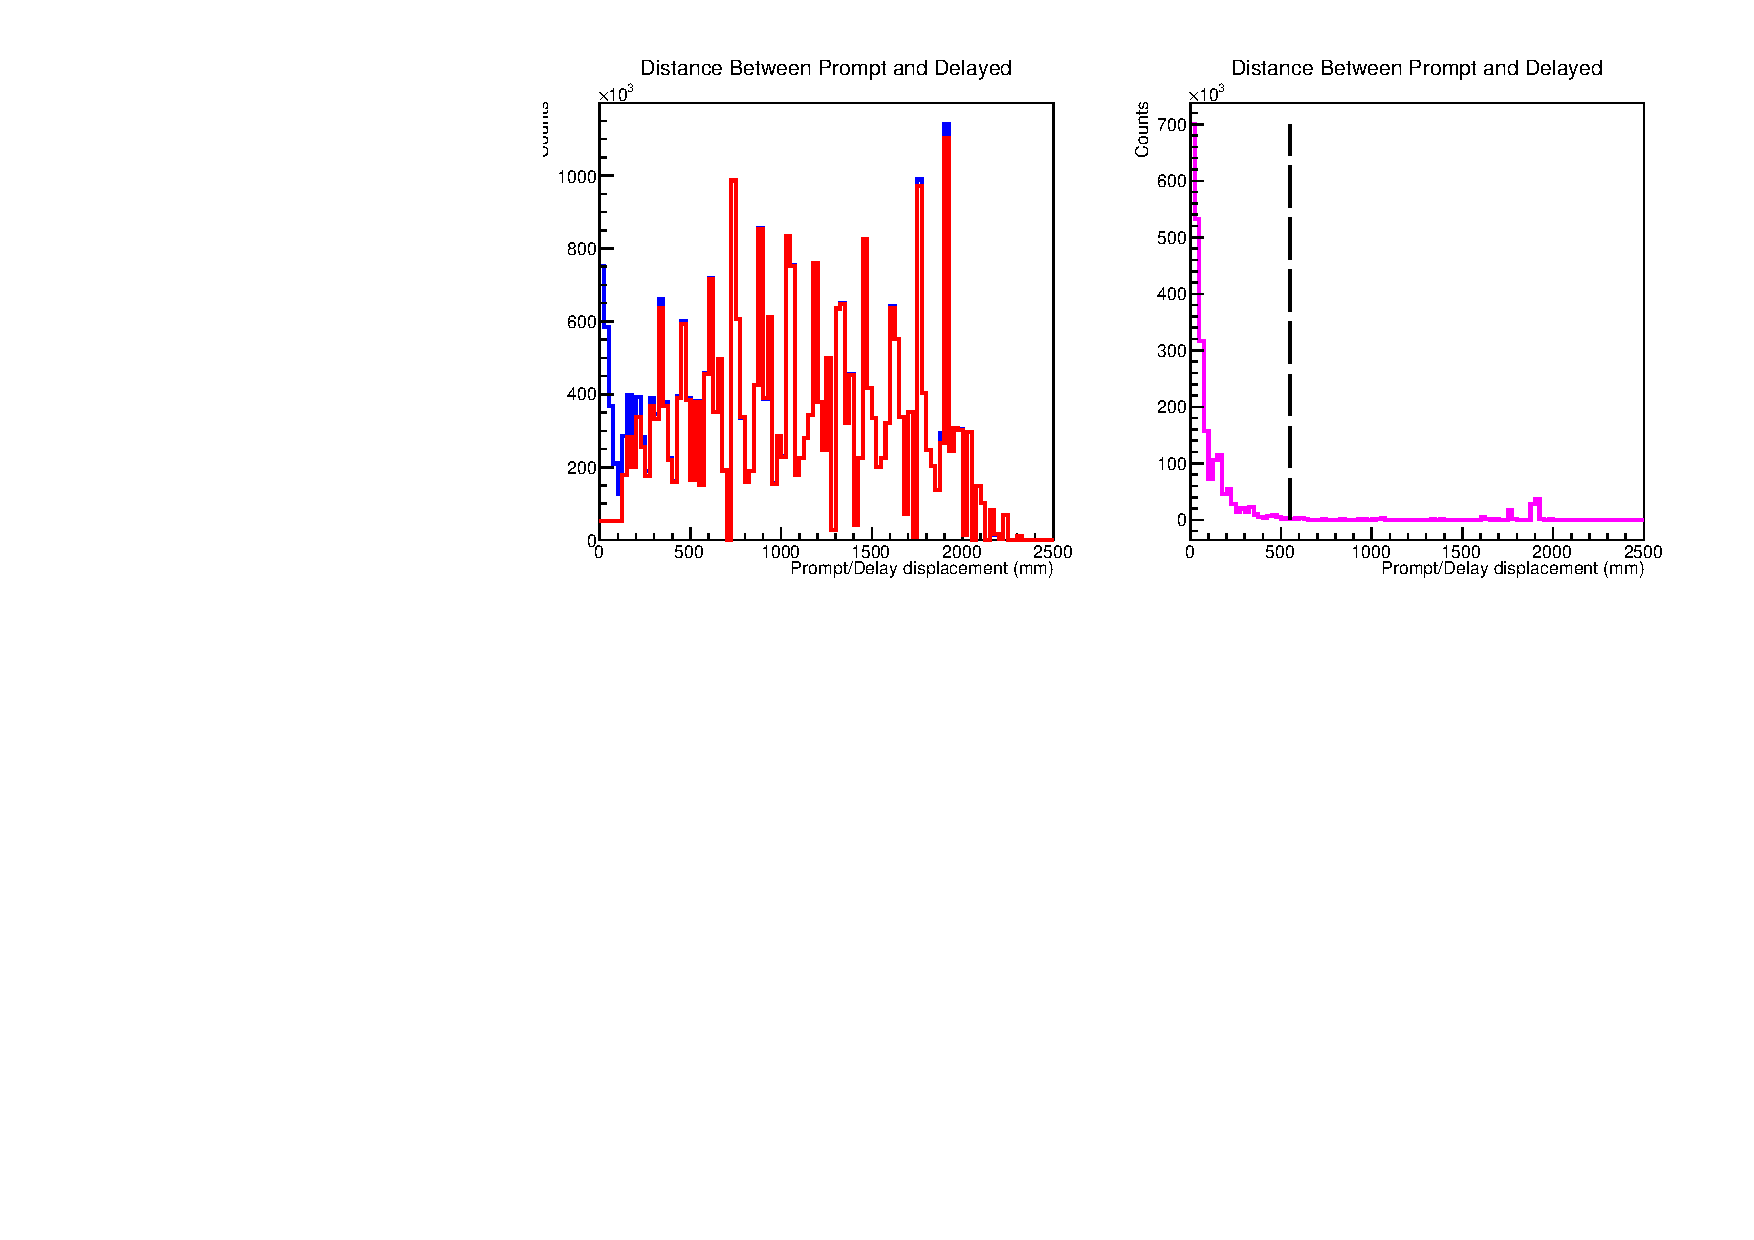
\includegraphics[width=1.0\textwidth]{../figures/distance_cut.pdf}
\caption{\label{fig:deltaD}Plots illustrating distribution of displacement between prompt and delayed BiPo-214 events. (Left)Distribution of prompt/delayed displacements (blue) and accidental (red) prompt/delayed displacements. (Right) Accidental-subtracted prompt/delayed displacements. Vertical line shows position of distance cut.}
\end{figure}

The accepted half-life of the $^{214}$Po decay is 0.1643~ms. The time difference between the prompt beta and delayed alpha candidates for this decay is limited to 0.01~ms$<$dt$<3\tau$ where $\tau=0.1643/\textrm{ln}(2)$~ms, the lifetime of $^{214}$Po. Figure \ref{fig:dt214} shows the $\Delta$t distribution. A fit to the half-life of $^{214}$Po is in good agreement with the accepted value.

The accepted half-life of the $^{212}$Po decay is 299~ns. The time difference between the prompt beta and delayed alpha candidates for this decay is limited to 700~ns$<$dt$<1.7~\mu$s. The time distribution (see Figure \ref{fig:dt212}) below 650~ns is distorted by artifacts of the length of the waveforms and an analysis hold off time as well as hardware trigger effects.  For this reason, a 700~ns software veto after each cluster has been imposed  A fit to the half-life of $^{212}$Po is in good agreement with the accepted value. 

Accidental subtraction is performed using a time offset window. For both alpha decays the offset window starts 10$\times\tau_{214}\approx2.4~ms$ forward from the alpha. The length of the accidentals offset window is set to be 12 times the length of the window for the prompt signal to accumulate more statistics. The accidentals histogram is then scaled by 1/12 to account for this. Other than the timing differences, the signals in the accidentals window are treated exactly the same as those in the prompt window, being subjected to exactly the same cuts and conditions.

The delayed monoenergetic alpha was limited to a single segment event, while the prompt beta with potentially high energy correlated gammas was allowed to fire multiple cells. A broad multiplicity cut was applied in the BiPoTreePlugin to limit the number of segments hit in the prompt event to less than 20. In the language of P2X prompt cluster multiplicity was limited to a size of 20 events or fewer.

\section{Software}
These plots were produced in a two step sequence. First, a TTree of BiPo candidates was produced for each run using the plugin framework from P2X. The plugin is called BiPoTreePlugin which lives in the PhysPulse directory. PhysPulse plugins operate on calibrated data, that is, data where pulse energy is calibrated to remove position dependence and where timing offsets due to hardware configurations and cable lengths have been removed. The cuts applied at the plugin level are relatively loose to allow for studies with restricting cuts later. Second, two programs are called to run over the BiPo TTrees and make the plots. The plots of variables such as energy and resolution versus time are made using the program ``BiPovsTime.C". The remaining plots that are averages over all time are made using ``BiPoPlotter.C".  Both of these ROOT macros use the same set of cuts on the data. See Sec. \ref{sec:cuts} for information on the cuts applied. For information on obtaining or viewing this code from the Github see Sec. \ref{sec:github} 
\subsection{Code used to generate plots}
The code required to do this analysis is all available on the Github (see Sec \ref{sec:github}). Production of the BiPo TTrees requires a working version of P2X. 
To build the BiPo TTrees run the script runBiPoTTreePlugin.sh
To plot results run BiPovsTime.C and BiPoPlotter.C from inside a ROOT terminal. 
\subsection{Github repository information\label{sec:github}}
The repository for P2X which includes the BiPoTree plugin can be cloned at\\ https://github.com/PROSPECT-collaboration/PROSPECT2x\_Analysis.git\\
The commit used in this analysis is \\
commit 8a232ab646935ac4d89cceaa38cf96e6c285dc72\\
Date:   Tue May 28 09:27:45 2019 -0700\\

The Github repository containing the analysis code includes a README file with instructions for reproducing these plots. The repository can be cloned at \\
https://github.com/PROSPECT-collaboration/BiPo-Analysis\\
The commit used to make these plots is\\
commit fde49de373613ae746682651d4639c44f66cc7d0\\
Date:   Fri May 31 13:12:05 2019 -0400\\
\newpage
%------------------------------
\section{Plots of interest}
\subsection{Energy versus segment plots}
\begin{figure}[!h]
\centering
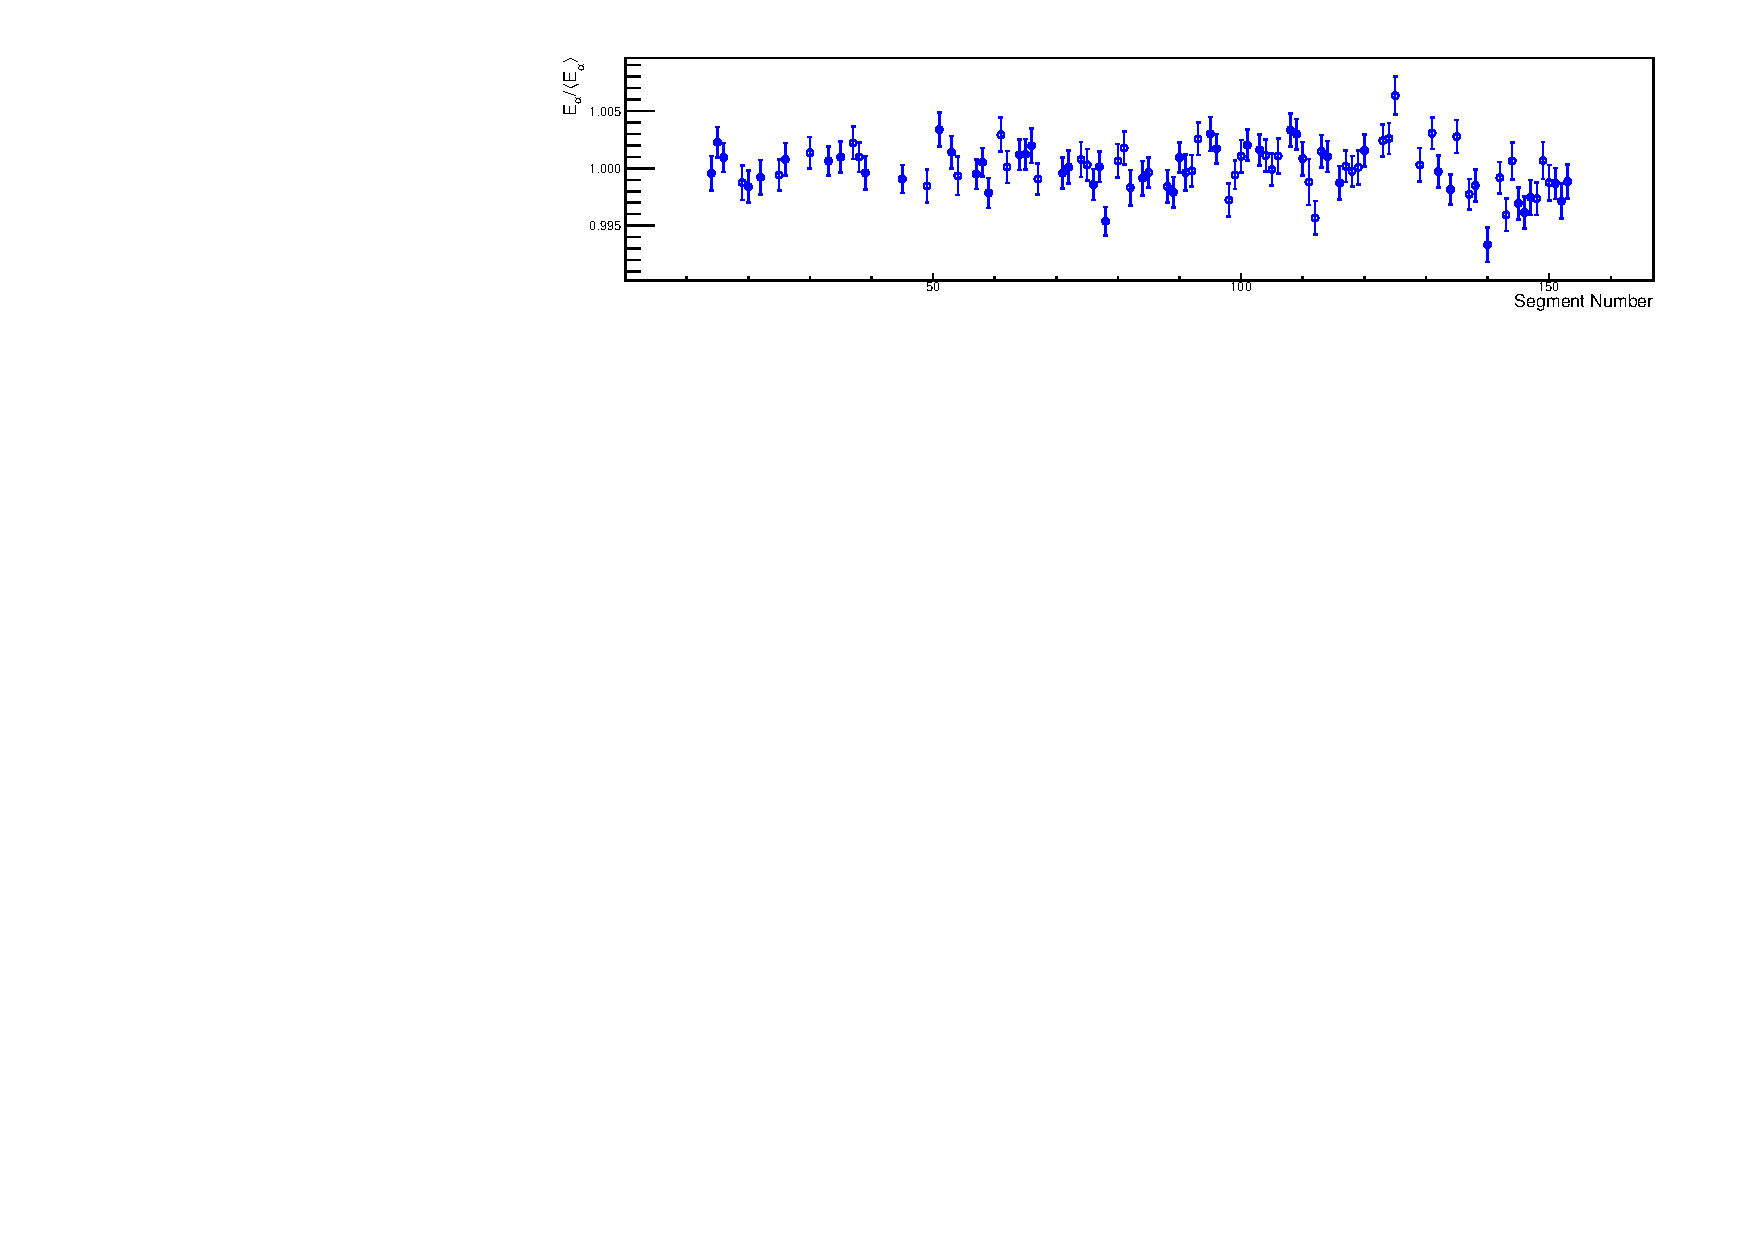
\includegraphics[width=1.05\textwidth]{figures/PubBiPo212EvsCell.pdf}
\caption{\label{fig:EvsCell212}Po-212 alpha energy versus segment number. The value is the mean of a Gaussian fit to the alpha energy peak and the error bar is the 1$\sigma$ width. Energy is normalized to the segment error-weighted average to highlight variations. Un-normalized weighted average energy is 1.05831$\pm$0.00015~MeV and $\chi^2$/NDF=274/90.}
\end{figure}
\begin{figure}[!h]
\centering
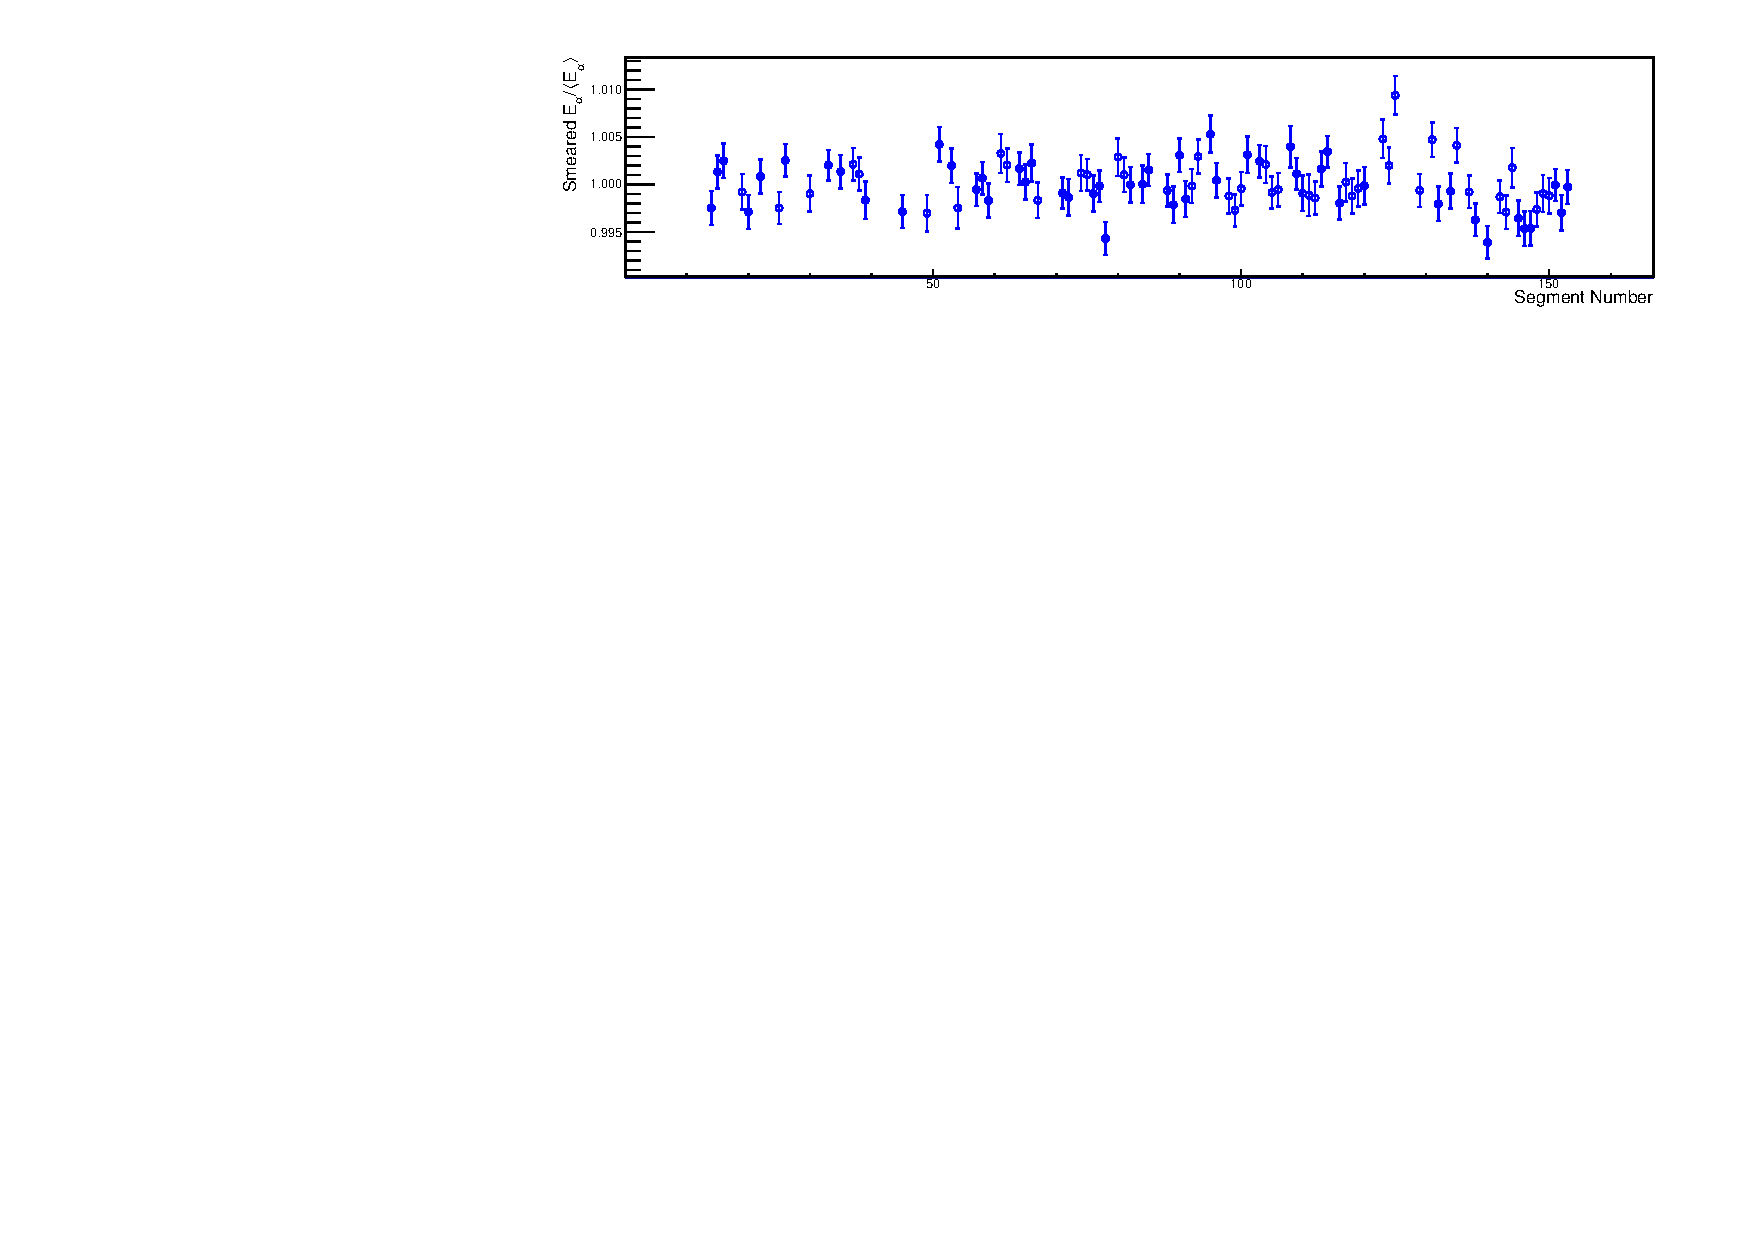
\includegraphics[width=1.05\textwidth]{figures/PubBiPo212EsmearvsCell.pdf}
\caption{\label{fig:EsmearvsCell212}Po-212 {\bf smeared} alpha energy versus segment number. The value is the mean of a Gaussian fit to the alpha energy peak and the error bar is the 1$\sigma$ width. Energy is normalized to the segment error-weighted average to highlight variations. Un-normalized weighted average energy is 1.05901$\pm$0.00020~MeV and $\chi^2$/NDF=175/90.}
\end{figure}
\begin{figure}[!h]
\centering
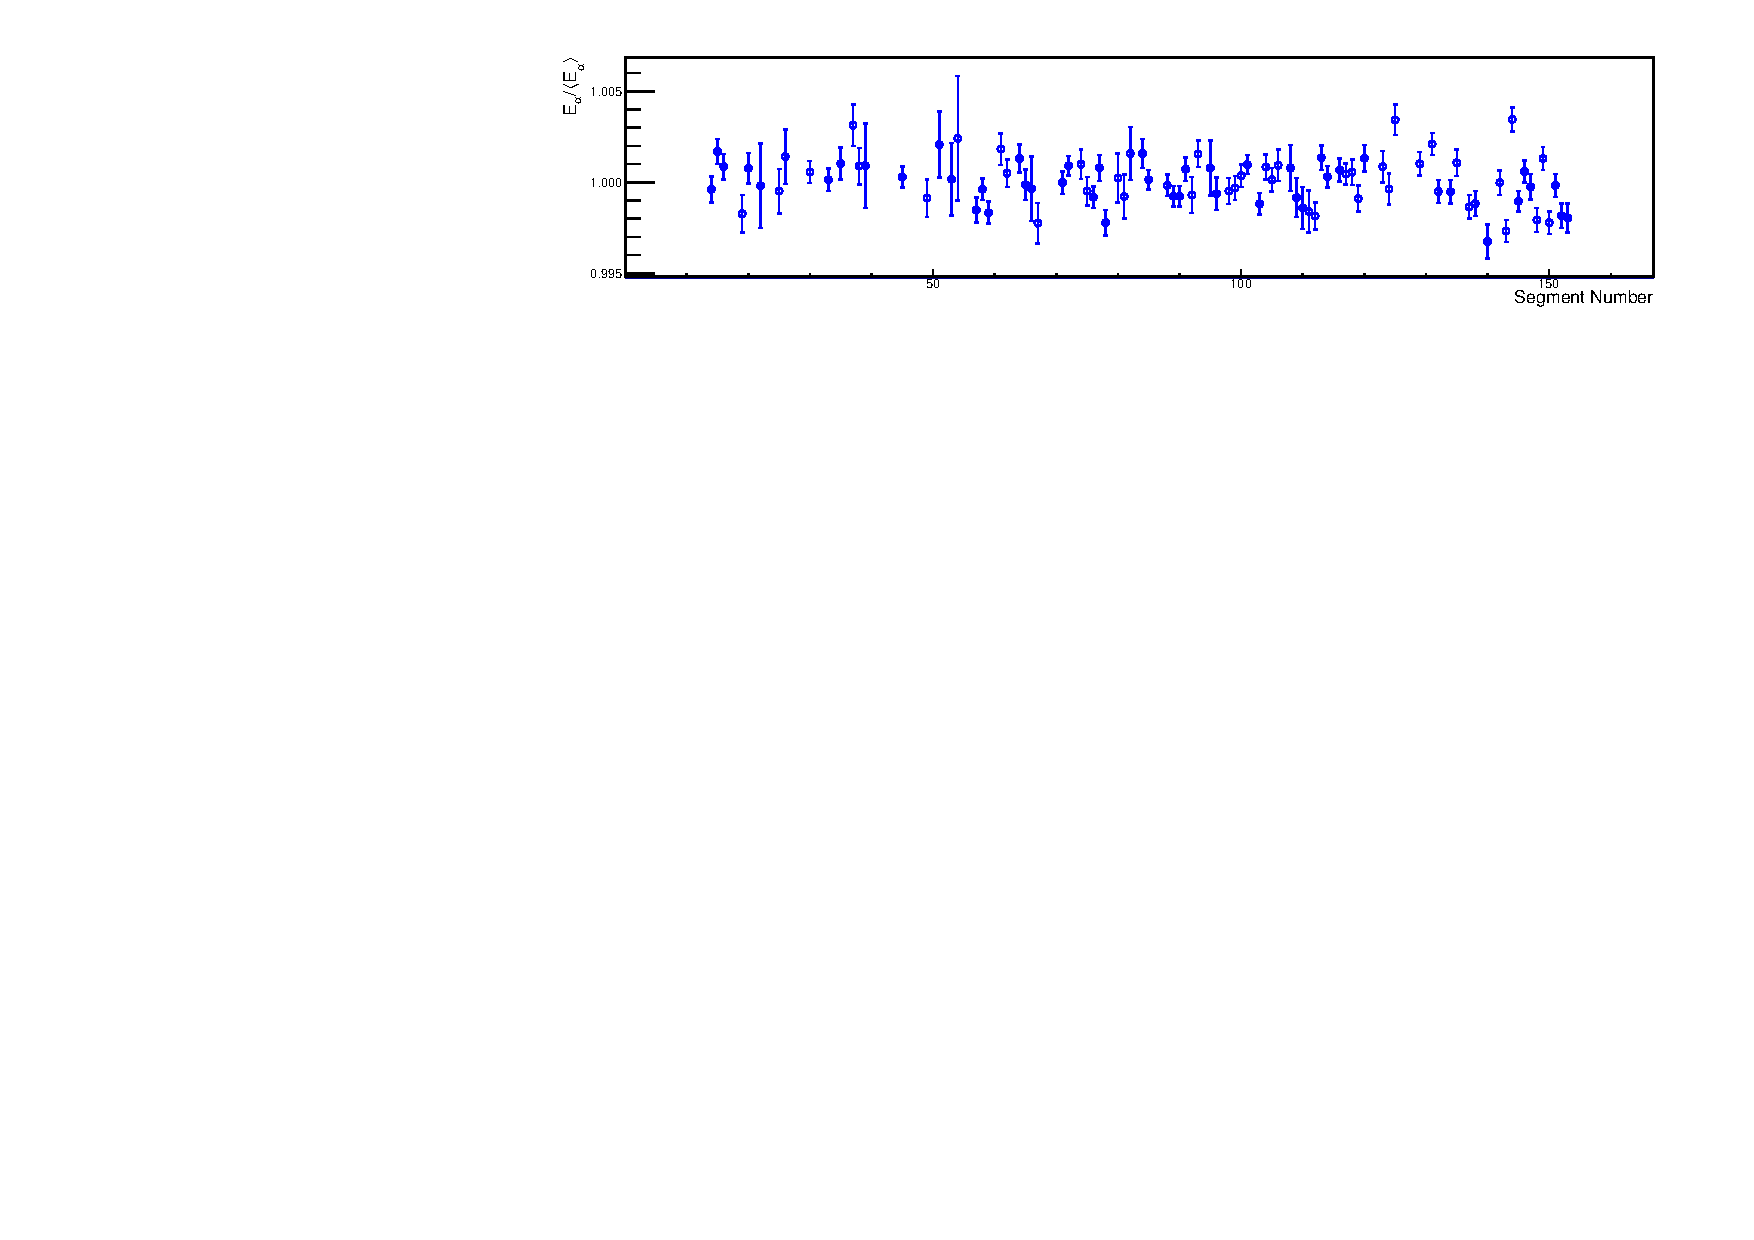
\includegraphics[width=1.05\textwidth]{figures/PubBiPo214EvsCell.pdf}
\caption{\label{fig:EvsCell214}Po-214 alpha energy versus segment number. The value is the mean of a Gaussian fit to the alpha energy peak and the error bar is the 1$\sigma$ width. Energy is normalized to the segment error-weighted average to highlight variations. Un-normalized weighted average energy is 0.84121$\pm$0.00006~MeV and $\chi^2$/NDF=291/90.} 
\end{figure}
\begin{figure}[!h]
\centering
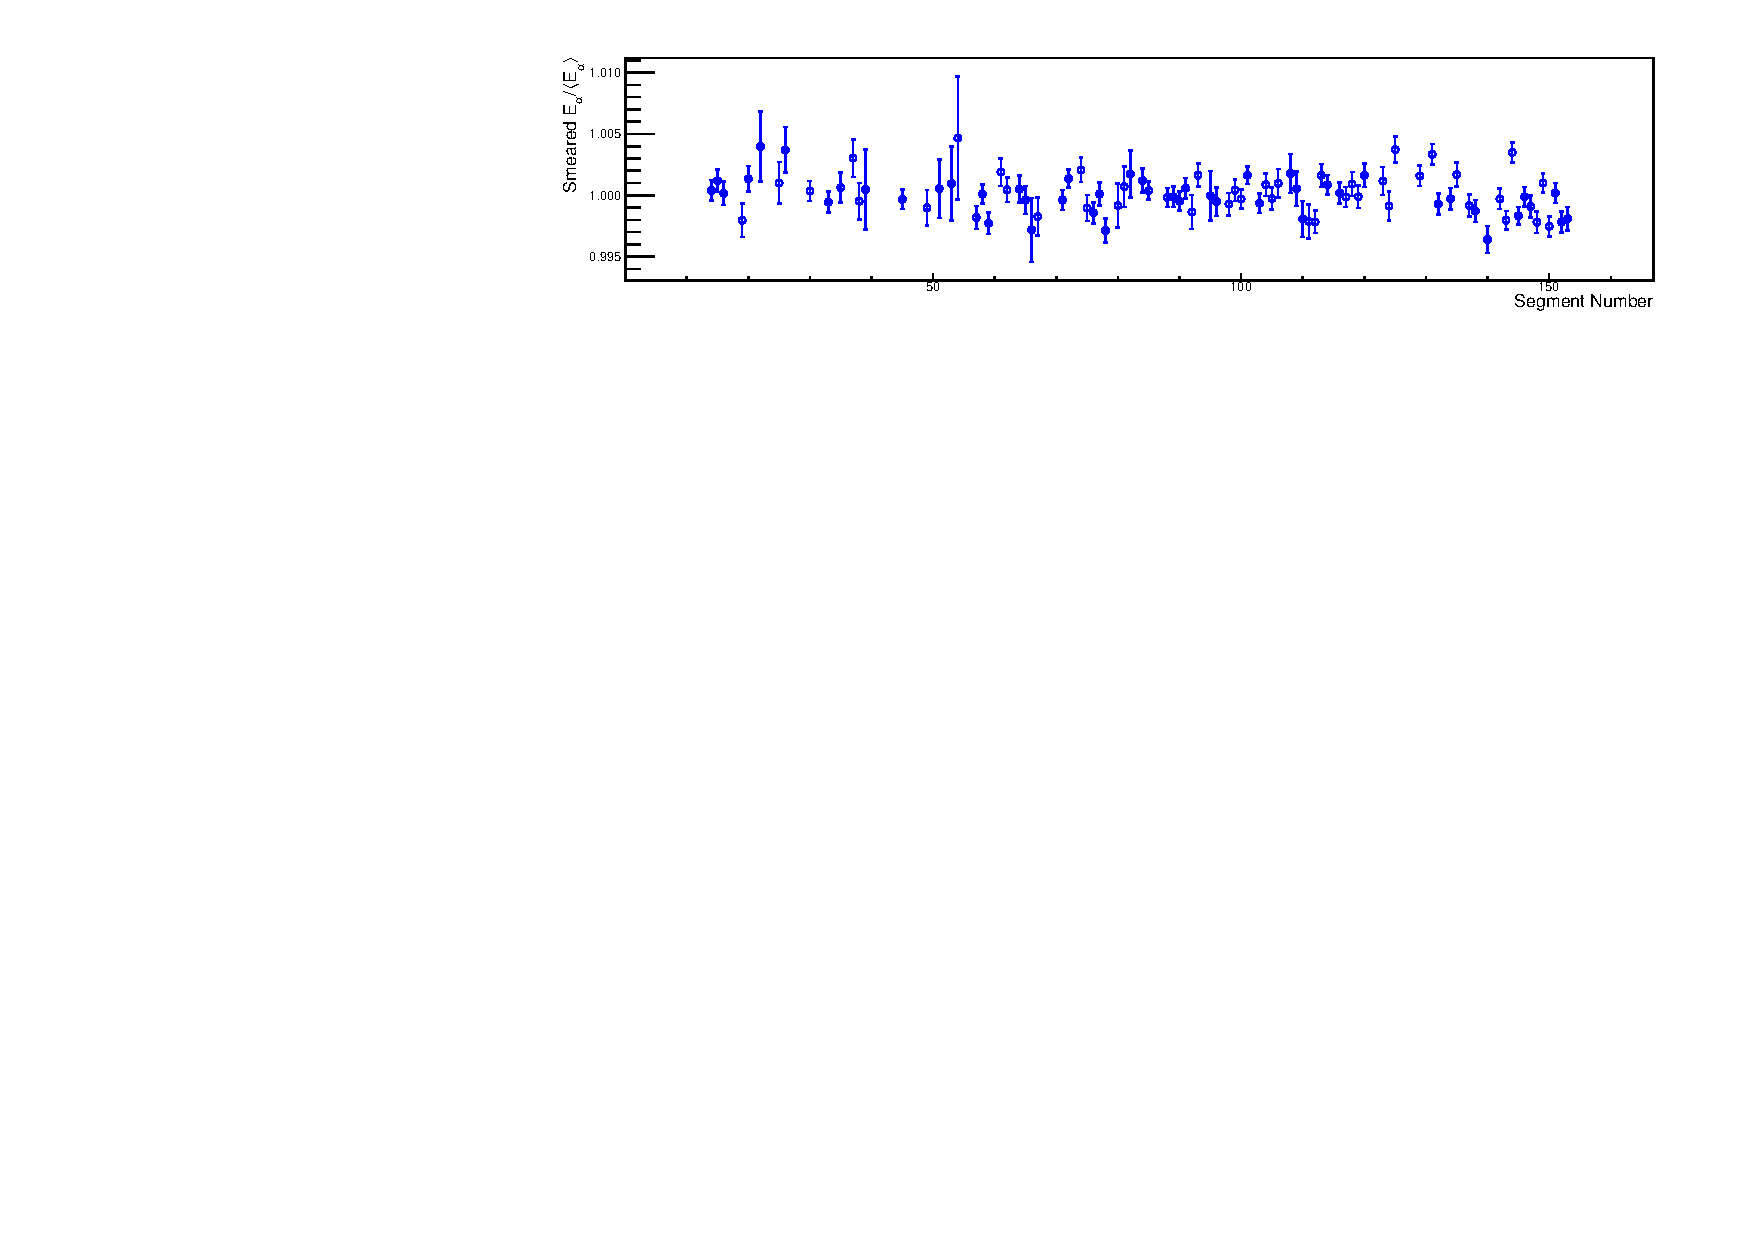
\includegraphics[width=1.05\textwidth]{figures/PubBiPo214EsmearvsCell.pdf}
\caption{\label{fig:EsmearvsCell214}Po-214 {\bf smeared} alpha energy versus segment number. The value is the mean of a Gaussian fit to the alpha energy peak and the error bar is the 1$\sigma$ width. Energy is normalized to the segment error-weighted average to highlight variations. Un-normalized weighted average energy is 0.84044$\pm$0.00009~MeV and $\chi^2$/NDF=202/90.} 
\end{figure}
\clearpage
\newpage

%------------------------------
\subsection{Energy resolution versus segment plots}
\begin{figure}[!h]
\centering
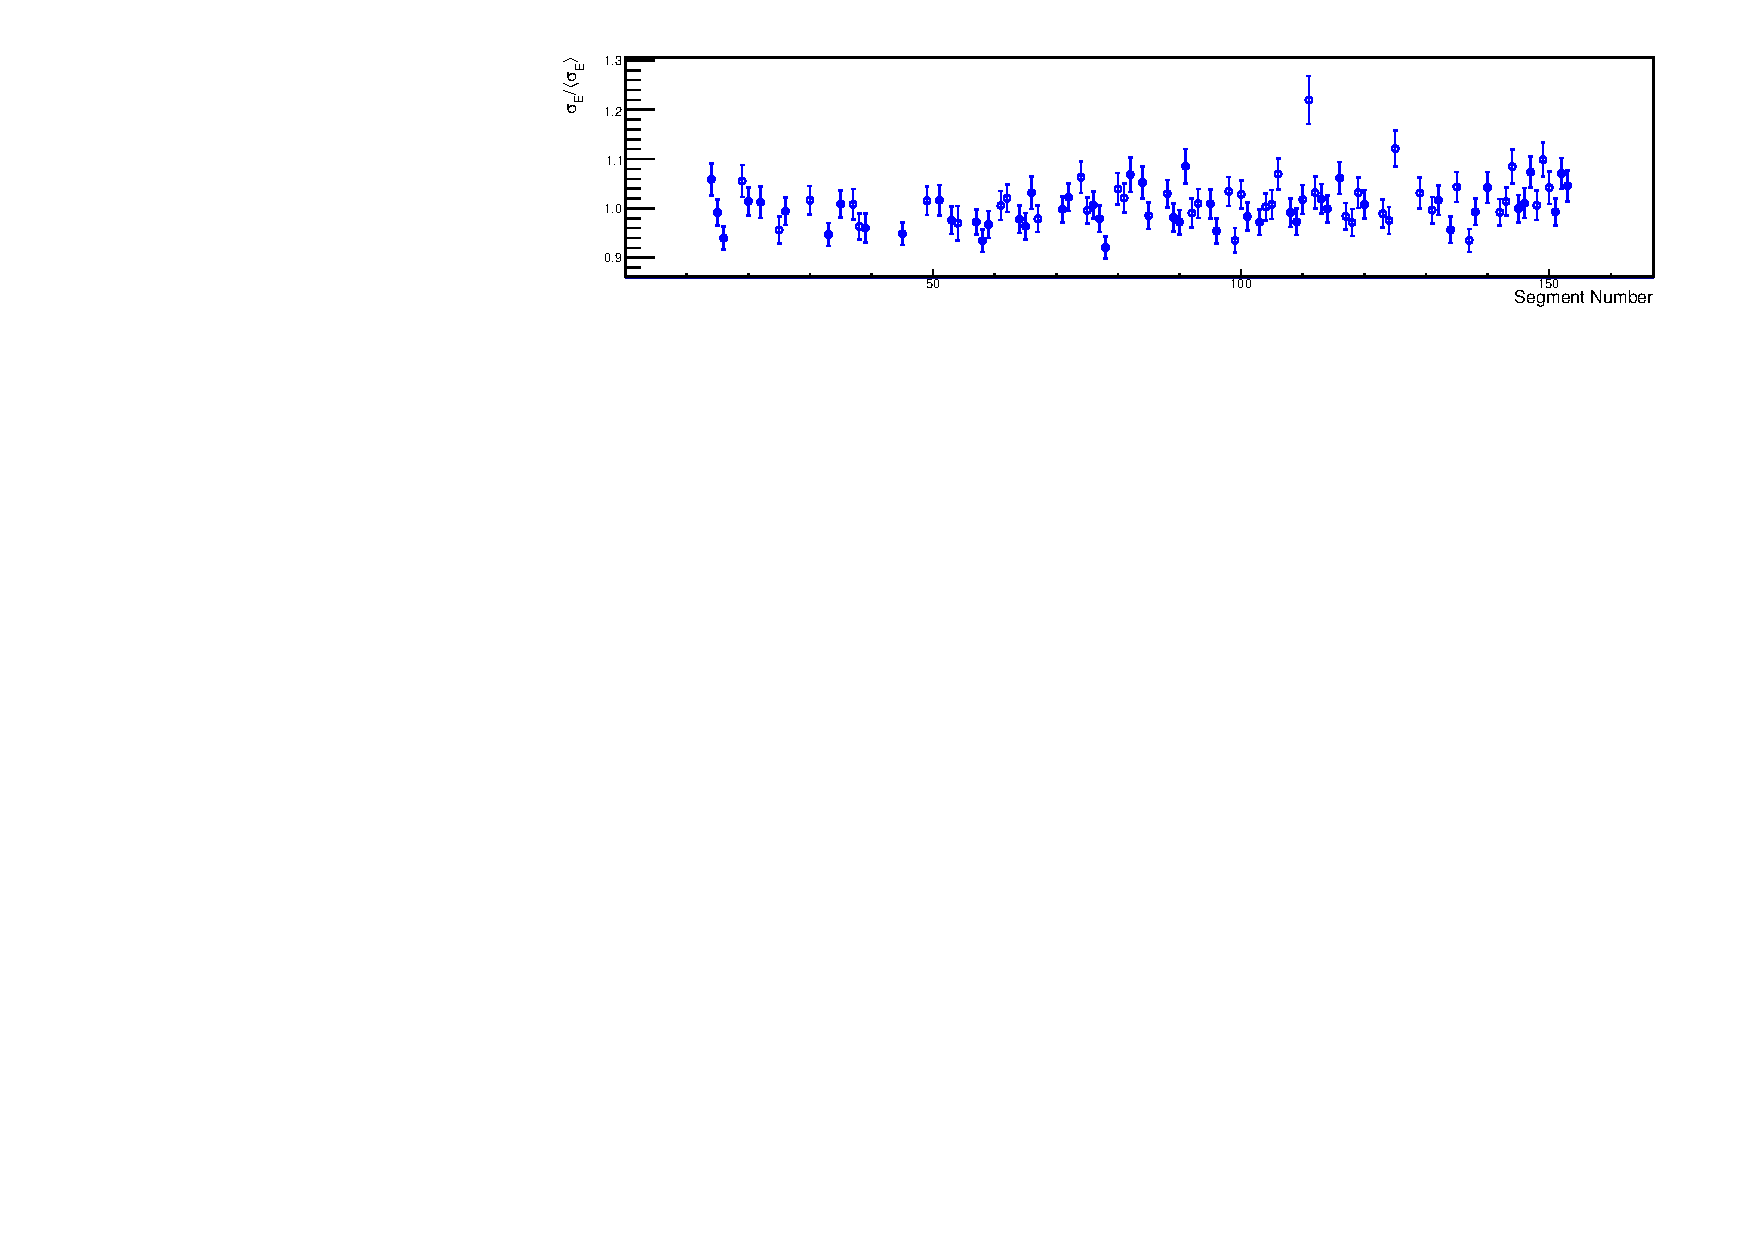
\includegraphics[width=1.05\textwidth]{figures/PubBiPo212EresvsCell.pdf}
\caption{\label{fig:EresvsCell212}Energy resolution versus segment using the alpha from Po-212 decay. The values are the 1$\sigma$ widths of a Gaussian fits to the alpha energy peaks and the error bars are the error on these values from the fit. Values are normalized to the segment error-weighted average to highlight variations. Un-normalized weighted average energy width is 0.04572$\pm$0.00009~MeV and $\chi^2$/NDF=1566/90.  In general, the higher width segments are those outfitted with ET tubes.}
\end{figure}
\begin{figure}[!h]
\centering
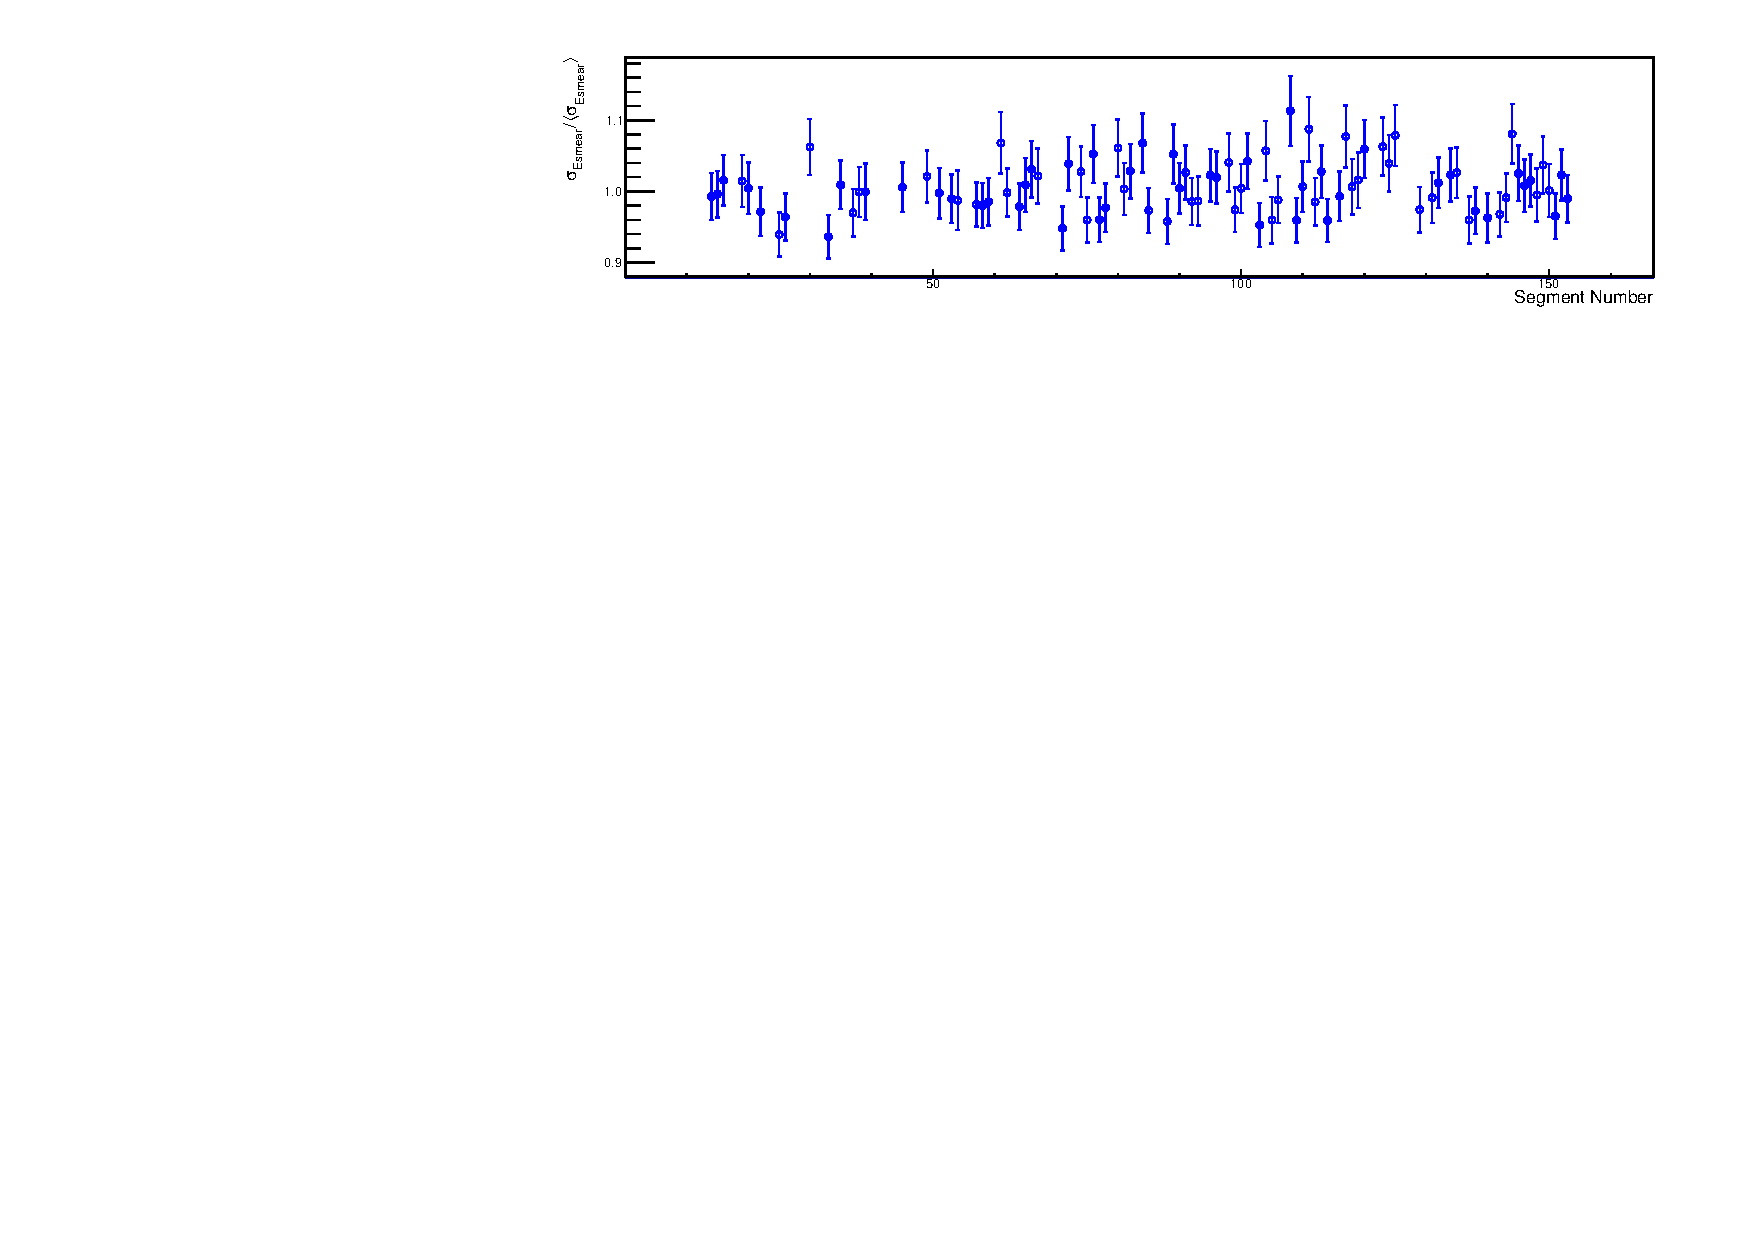
\includegraphics[width=1.05\textwidth]{figures/PubBiPo212EsmearresvsCell.pdf}
\caption{\label{fig:EsmearresvsCell212}{\bf Smeared} energy resolution versus segment using the alpha from Po-212 decay. The values are the 1$\sigma$ widths of a Gaussian fits to the alpha energy peaks and the error bars are the error on these values from the fit. Values are normalized to the segment error-weighted average to highlight variations. Un-normalized weighted average energy width is 0.05774$\pm$0.00021~MeV and $\chi^2$/NDF=88/90.  In general, the higher width segments are those outfitted with ET tubes.}
\end{figure}
\begin{figure}[!h]
\centering
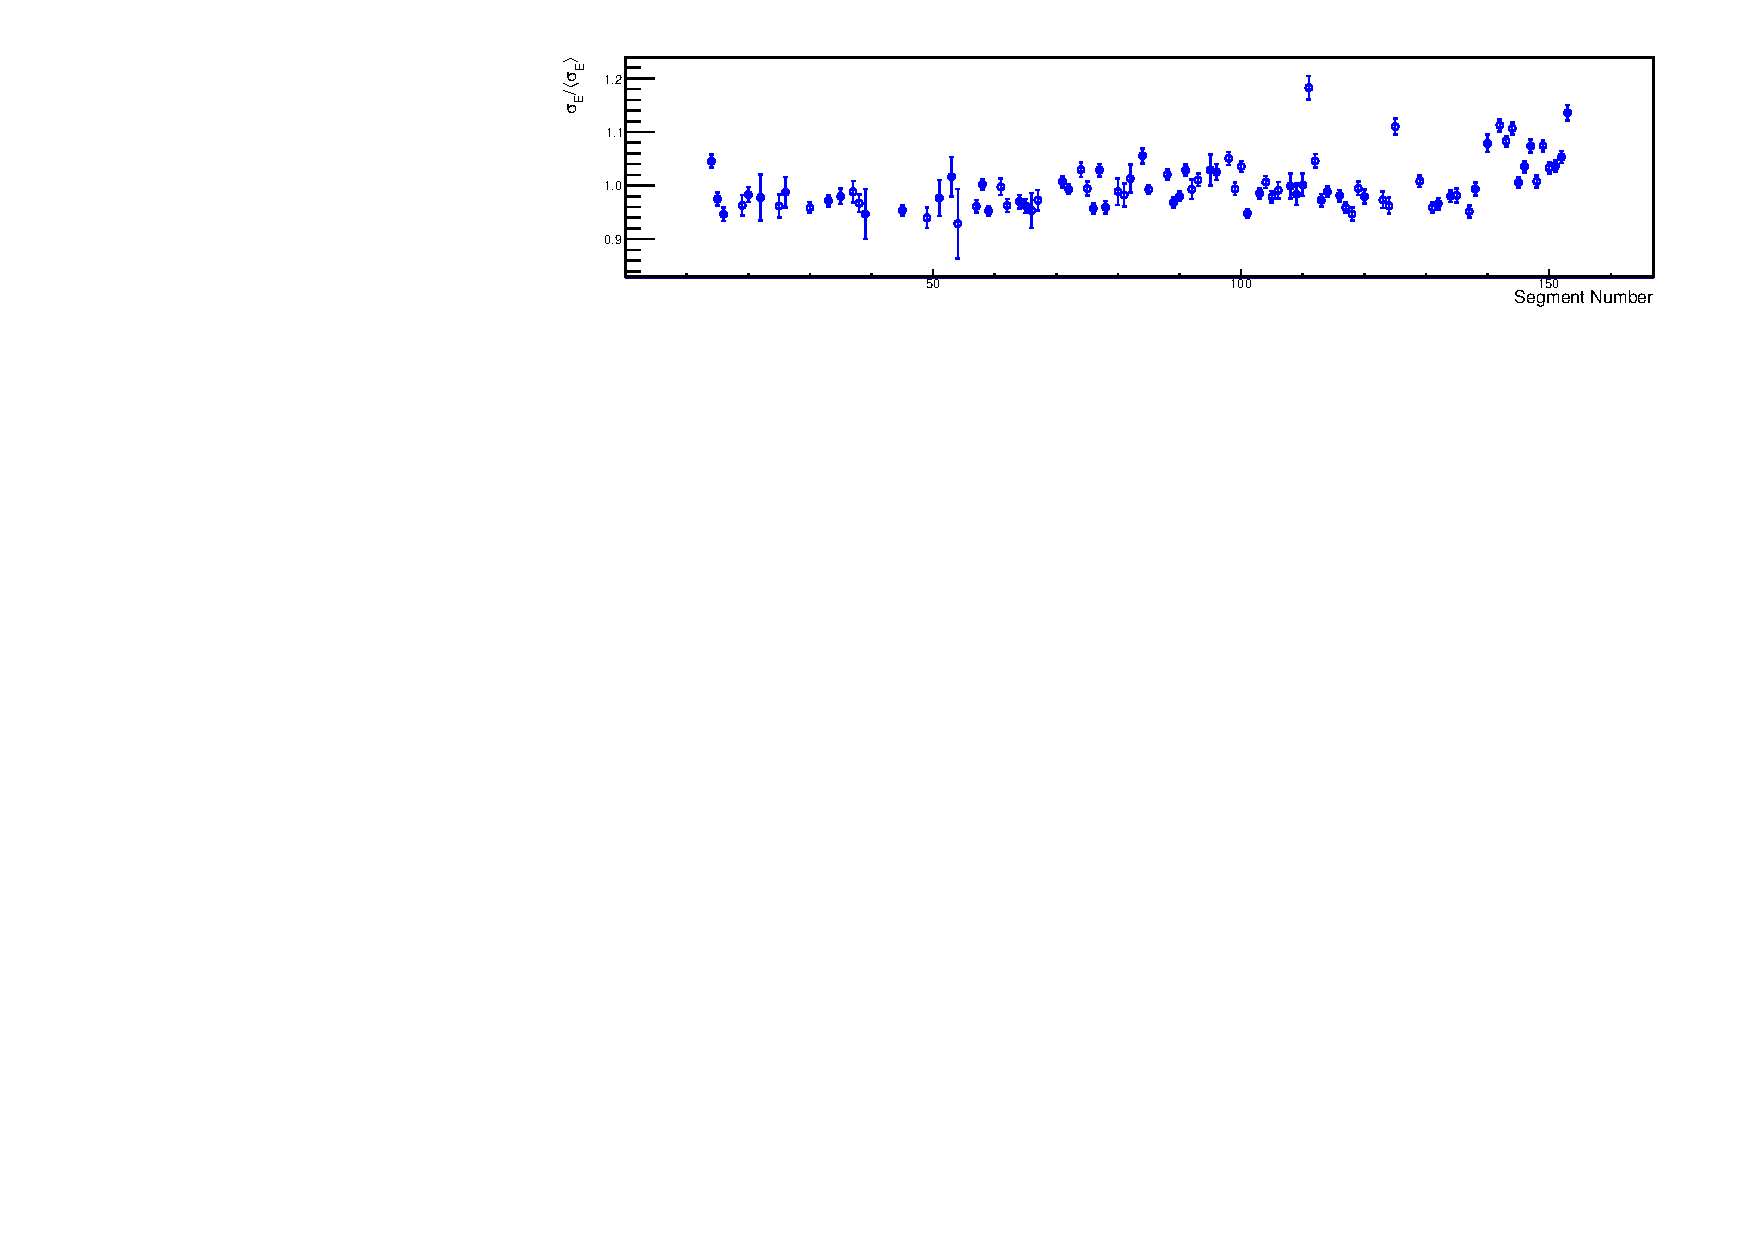
\includegraphics[width=1.05\textwidth]{figures/PubBiPo214EresvsCell.pdf}
\caption{\label{fig:EresvsCell214}Energy resolution versus segment using the alpha from Po-214 decay. The values are the 1$\sigma$ widths of a Gaussian fits to the alpha energy peaks and the error bars are the error on these values from the fit. Values are normalized to the segment error-weighted average to highlight variations. Un-normalized weighted average energy width is 0.04427$\pm$0.00006~MeV and $\chi^2$/NDF=1120/90.  In general, the higher width segments are those outfitted with ET tubes.}
\end{figure}
\begin{figure}[!h]
\centering
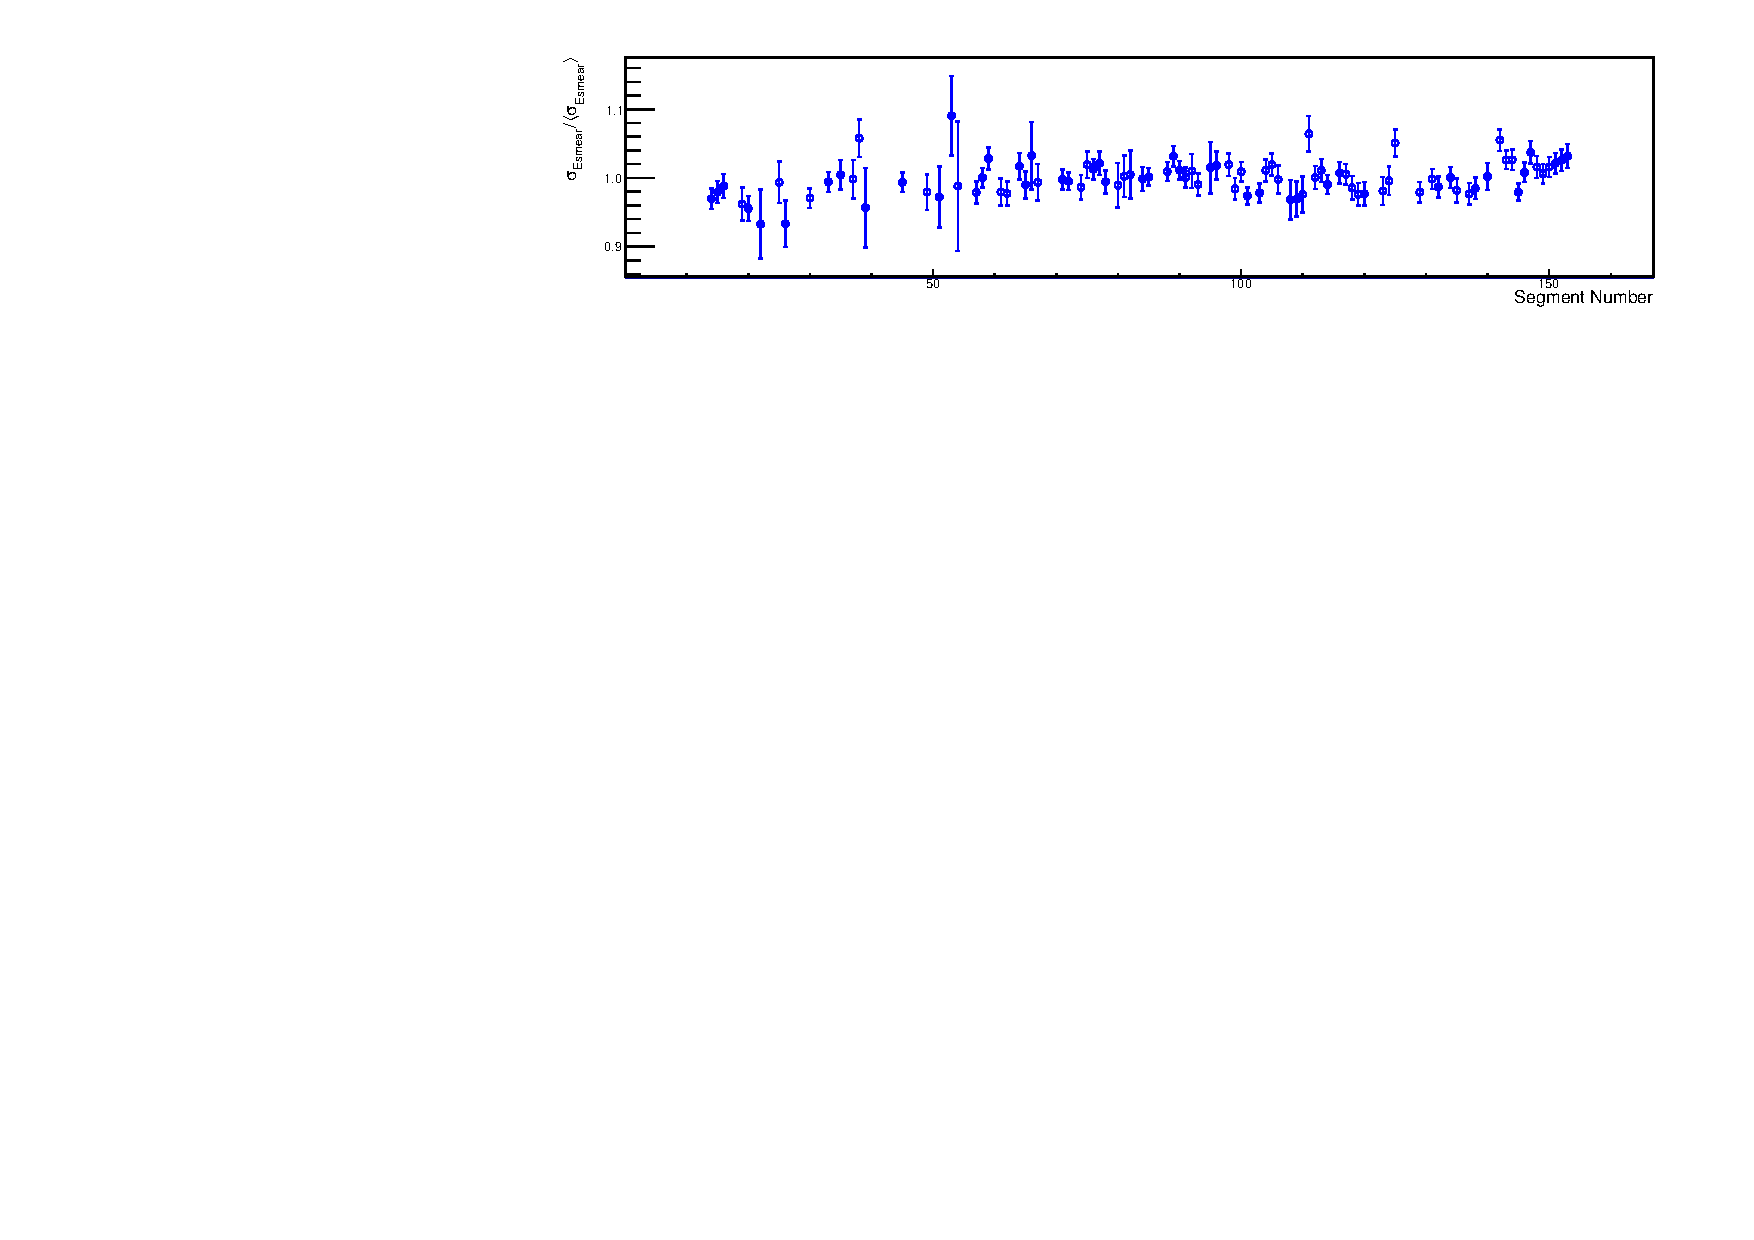
\includegraphics[width=1.05\textwidth]{figures/PubBiPo214EsmearresvsCell.pdf}
\caption{\label{fig:EsmearresvsCell214}{\bf Smeared} energy resolution versus segment using the alpha from Po-214 decay. The values are the 1$\sigma$ widths of a Gaussian fits to the alpha energy peaks and the error bars are the error on these values from the fit. Values are normalized to the segment error-weighted average to highlight variations. Un-normalized weighted average energy width is 0.05230$\pm$0.00010~MeV and $\chi^2$/NDF=134/90.  In general, the higher width segments are those outfitted with ET tubes.}
\end{figure}
\clearpage
\newpage
%------------------------------
\subsection{Z-position resolution versus segment plots}
\begin{figure}[!h]
\centering
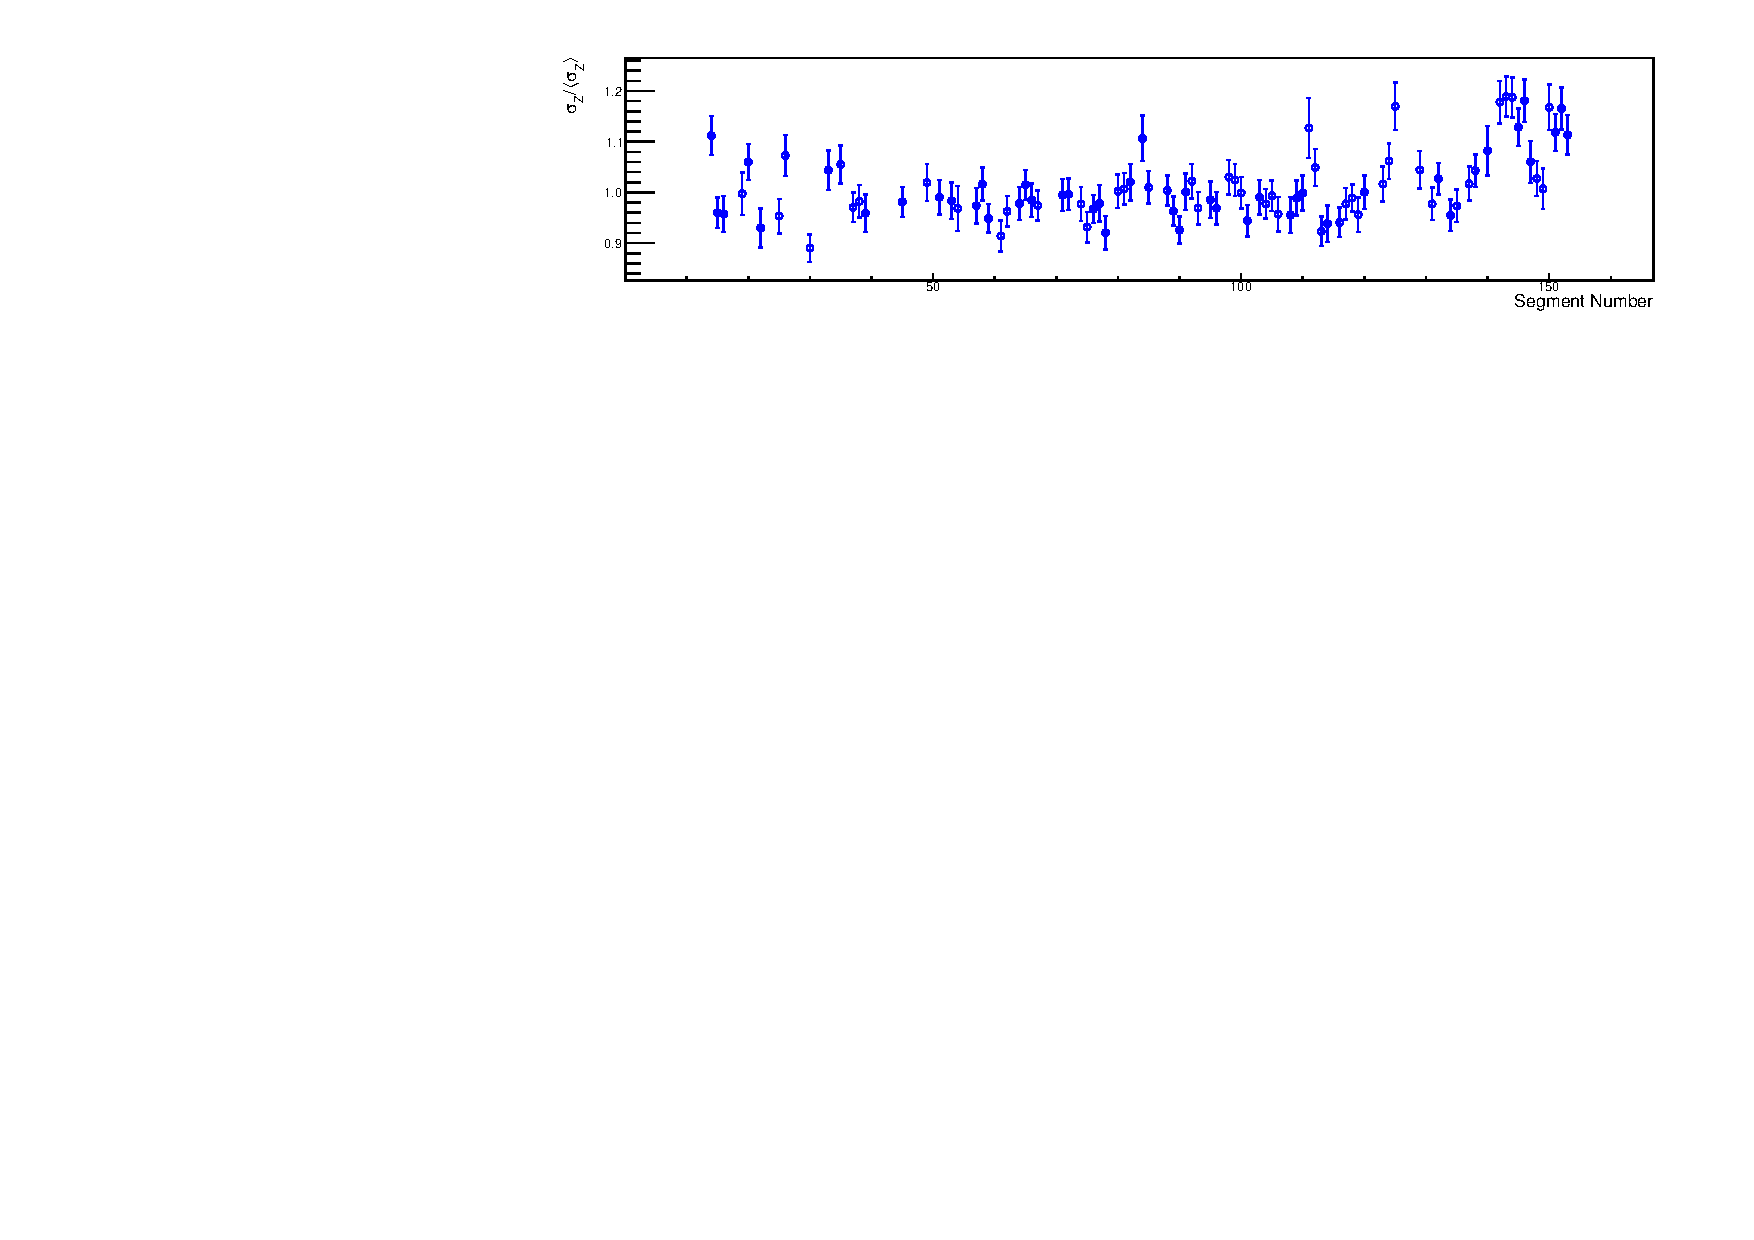
\includegraphics[width=1.05\textwidth]{figures/PubBiPo212dZWidthvsCell.pdf}
\caption{\label{fig:ZresvsCell212}Z-position resolution versus segment using the beta, alpha from Bi-212, Po-212. The values are the 1$\sigma$ widths of a Gaussian fits to the alpha minus beta Z-distance distributions and the error bars are the error on these values from the fit. Outliers with larger position resolution are primarily the outer layer segments outfitted with ET-tubes. Values are normalized to the segment error-weighted average to highlight variations. Un-normalized weighted average $\Delta$Z width is 43.18$\pm$0.15~mm and $\chi^2$/NDF=298/90.}
\end{figure}
\begin{figure}[!h]
\centering
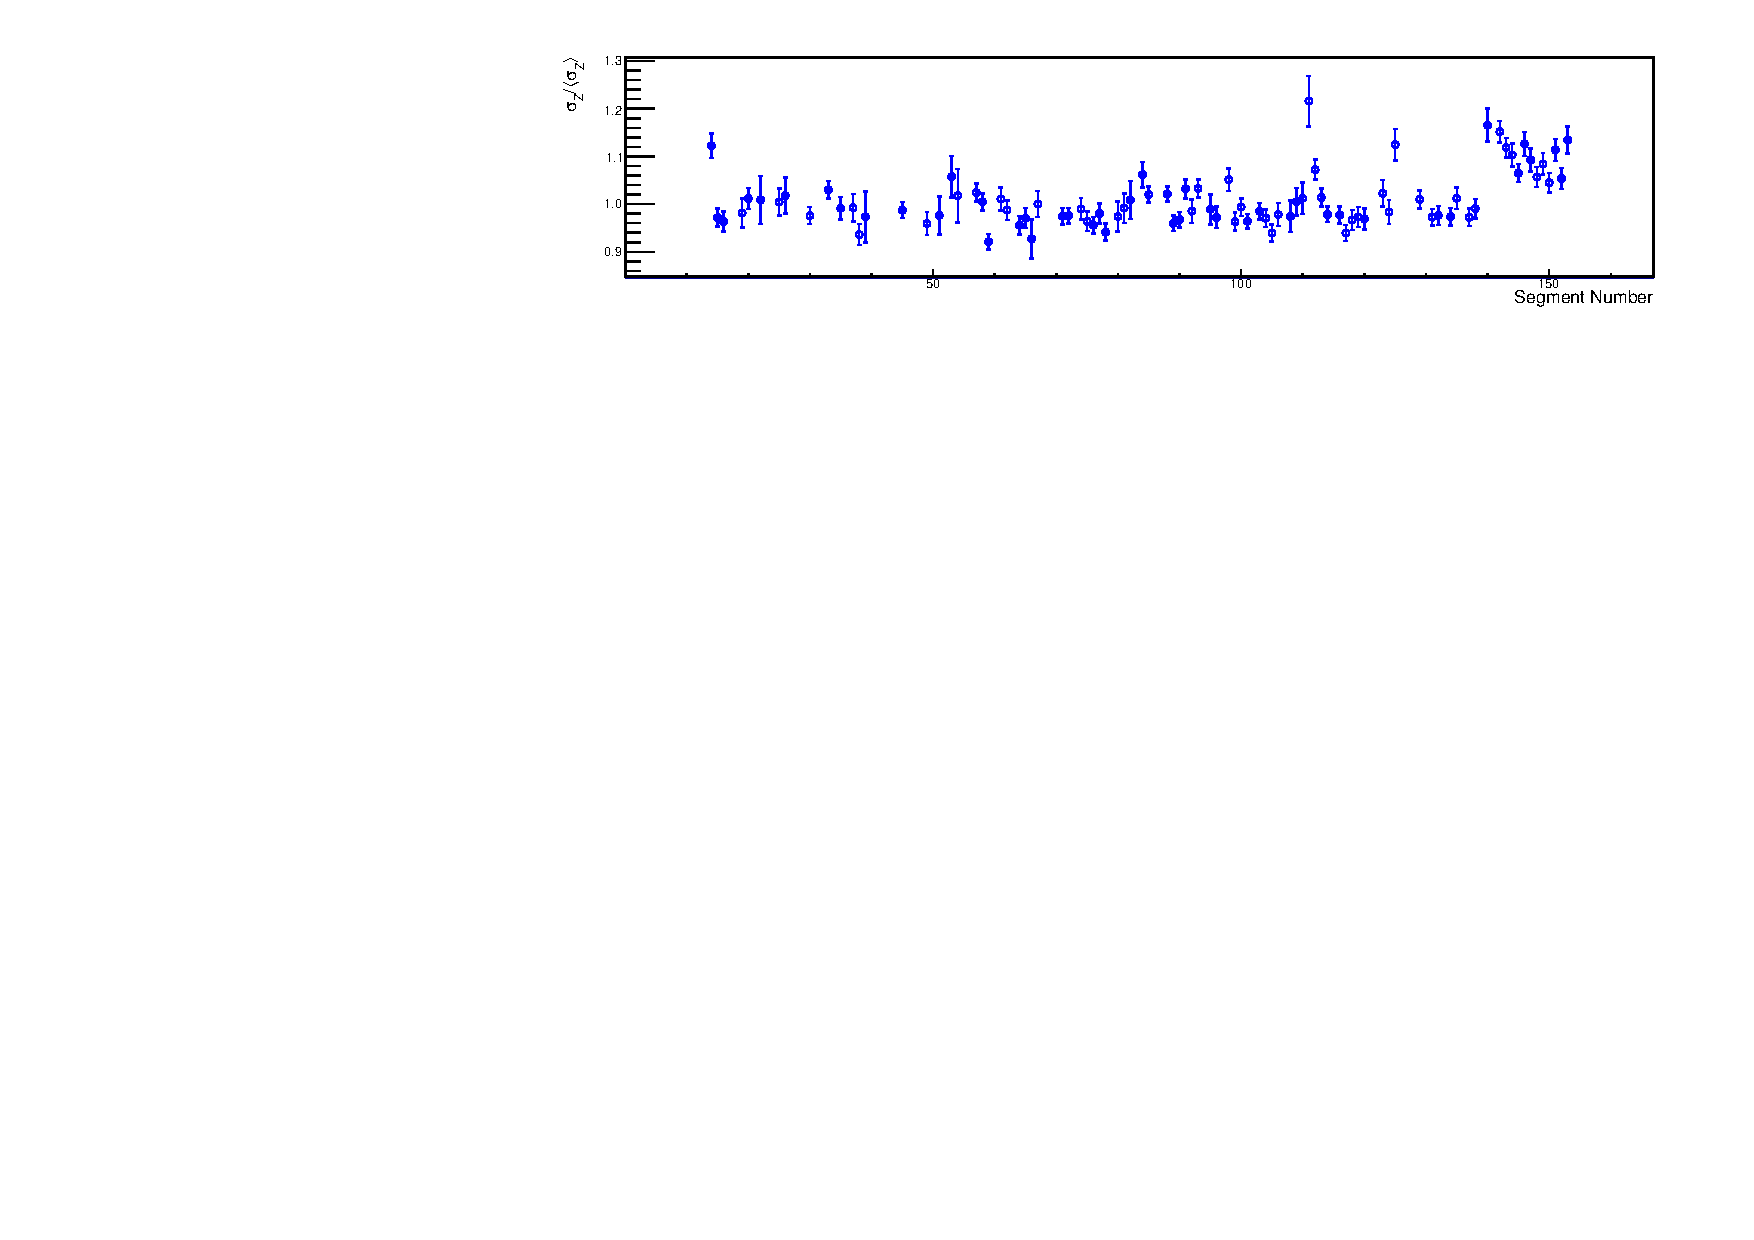
\includegraphics[width=1.05\textwidth]{figures/PubBiPo214dZWidthvsCell.pdf}
\caption{\label{fig:ZresvsCell214}Z-position resolution versus segment using the beta, alpha from Bi-214, Po-214. The values are the 1$\sigma$ widths of a Gaussian fits to the alpha minus beta Z-distance distributions and the error bars are the error on these values from the fit. In general, outliers with larger position resolution are primarily the outer layer segments outfitted with ET-tubes. Values are normalized to the segment error-weighted average to highlight variations. Un-normalized weighted average $\Delta$Z width is 45.6$\pm$0.1~mm and $\chi^2$/NDF=496/90.}
\end{figure}
\clearpage
\newpage
%------------------------------
\subsection{Z-distribution RMS width versus segment plots}
\begin{figure}[!h]
\centering
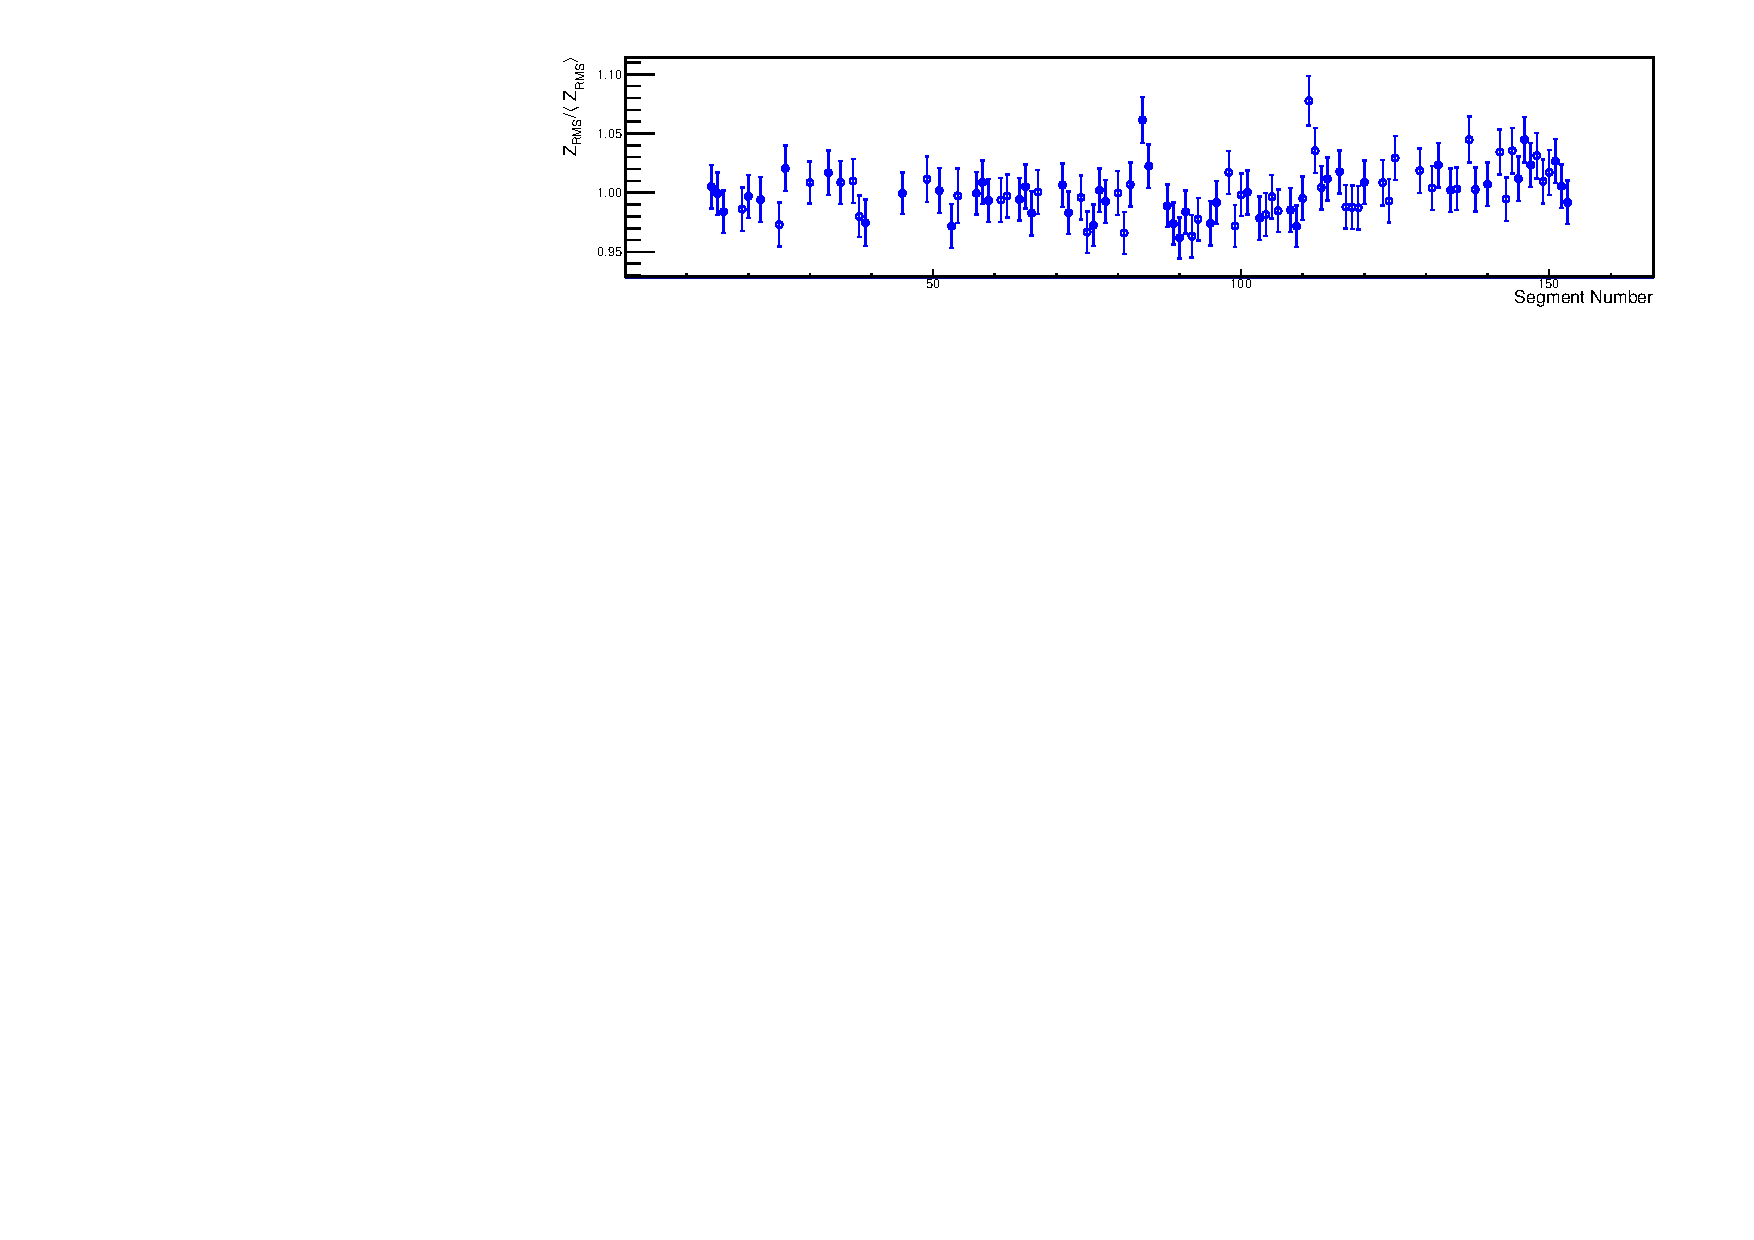
\includegraphics[width=1.05\textwidth]{figures/PubBiPo212ZRMSvsCell.pdf}
\caption{\label{fig:ZRMSvsCell212}RMS width of Z-distribution of Po-212 alphas versus segment. The error bars are the errors assigned by ROOT to the RMS values of the histograms. Values are normalized to the segment error-weighted average to highlight variations. Un-normalized weighted average Z$_{RMS}$ width is 348.2$\pm$0.7~mm and $\chi^2$/NDF=113/90. }
\end{figure}
\begin{figure}[!h]
\centering
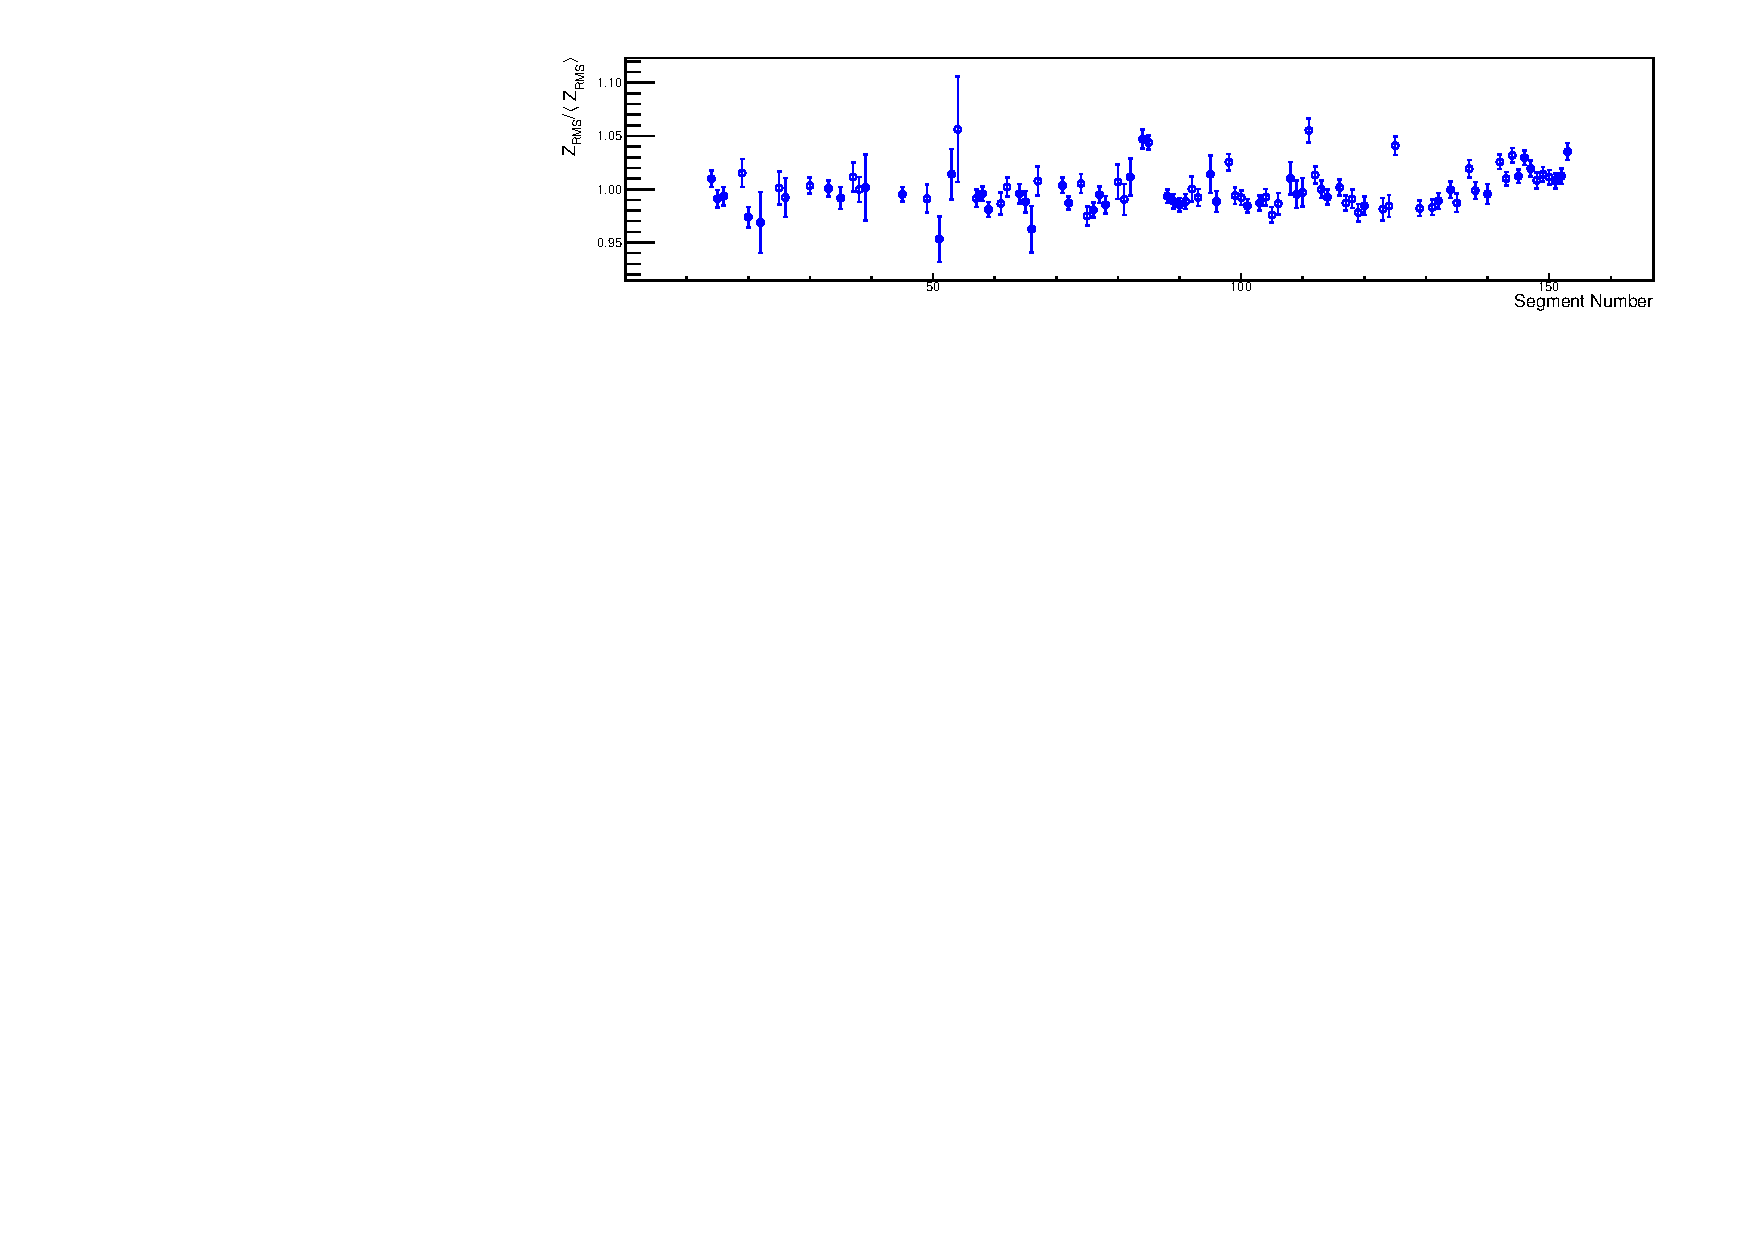
\includegraphics[width=1.05\textwidth]{figures/PubBiPo214ZRMSvsCell.pdf}
\caption{\label{fig:ZRMSvsCell214}RMS width of Z-distribution of Po-214 alphas versus segment. The error bars are the errors assigned by ROOT to the RMS values of the histograms. Values are normalized to the segment error-weighted average to highlight variations. Un-normalized weighted average Z$_{RMS}$ width is 347.4$\pm$0.3~mm and $\chi^2$/NDF=374/90.}
\end{figure}
\clearpage
\newpage
%------------------------------
\subsection{Z-position distribution mean versus segment plots}
\begin{figure}[!h]
	\centering
	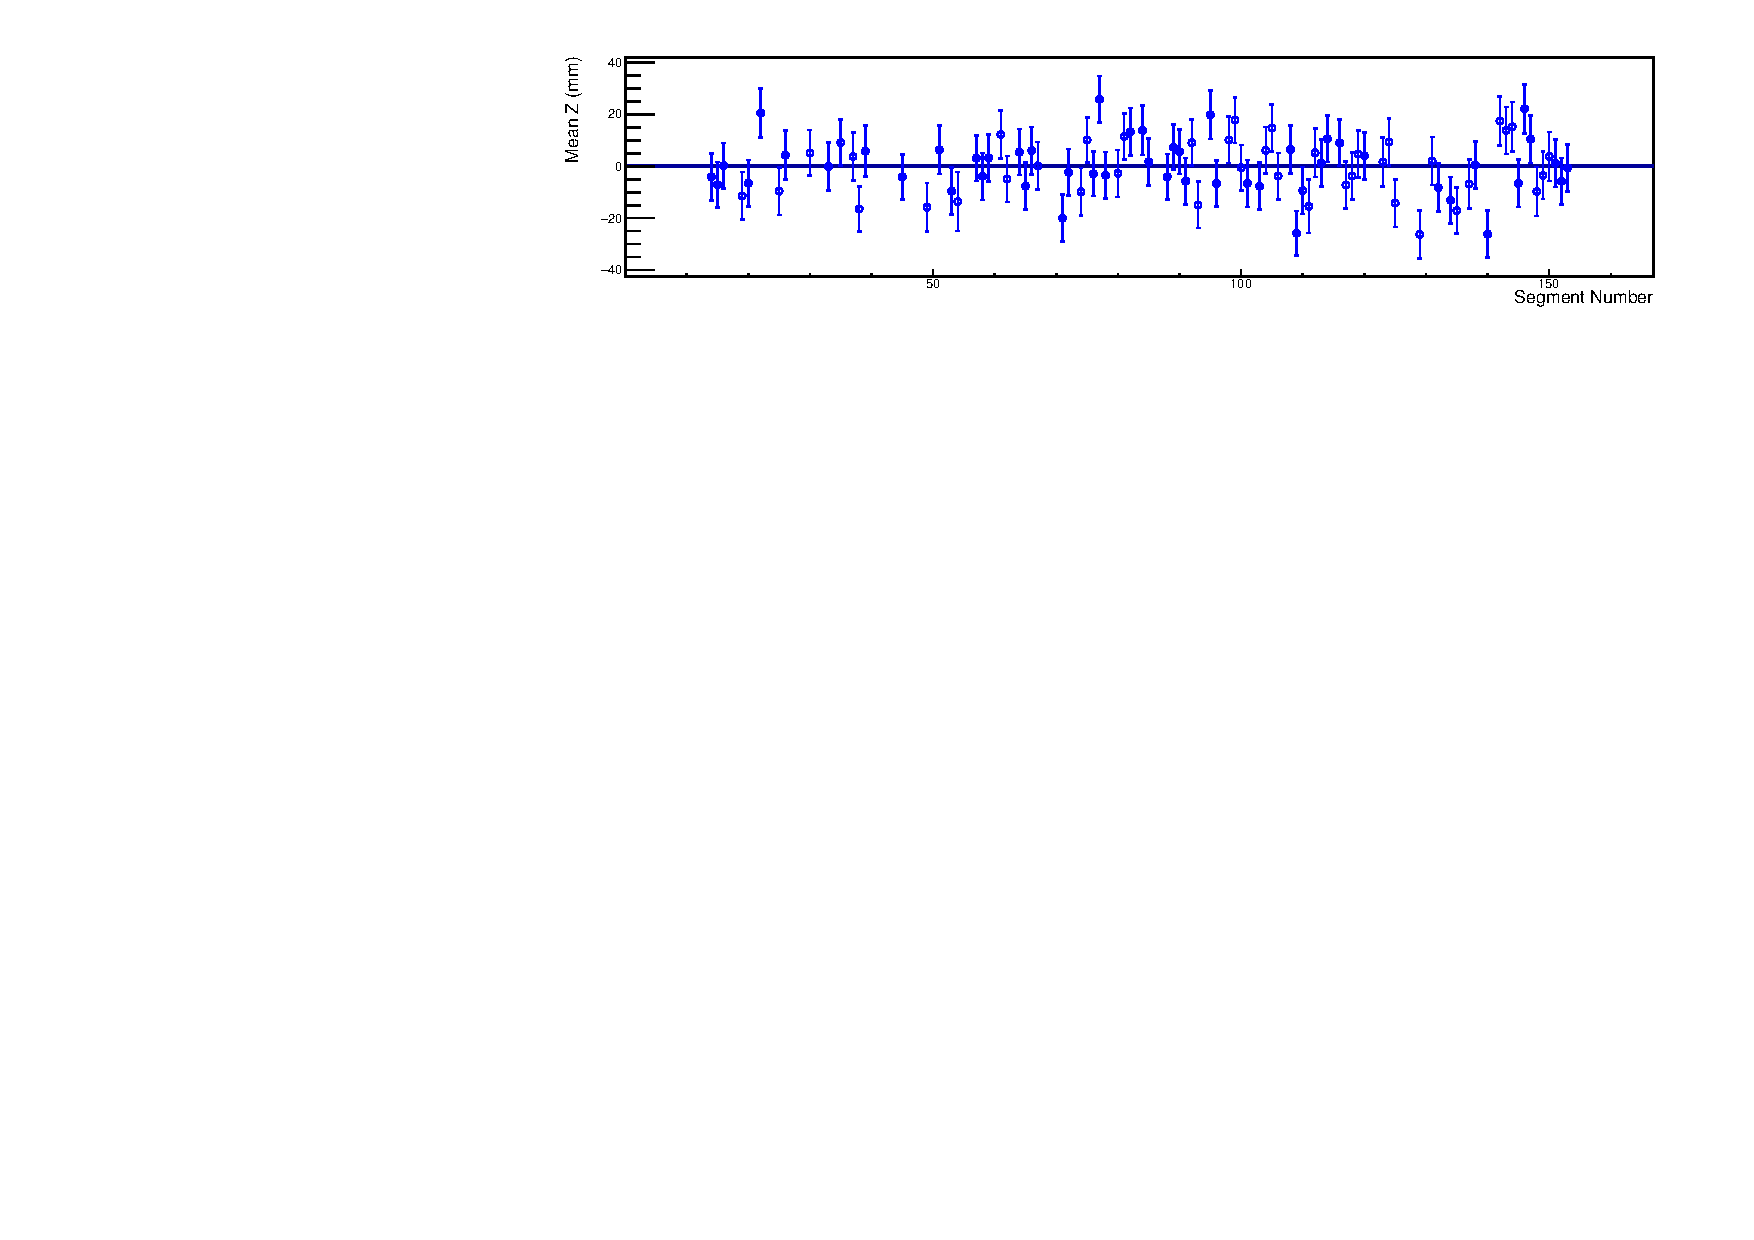
\includegraphics[width=1.05\textwidth]{figures/PubBiPo212meanZvsCell.pdf}
	\caption{\label{fig:meanZvsCell212}Mean of Z-position distribution of Po-212 alphas versus segment. The values are distributions averages and the error bars are the RMS of the distribution. The weighted average mean Z-position is 0.03$\pm$0.94~mm and $\chi^2$/NDF=139/90.   }
\end{figure}
\begin{figure}[!h]
	\centering
	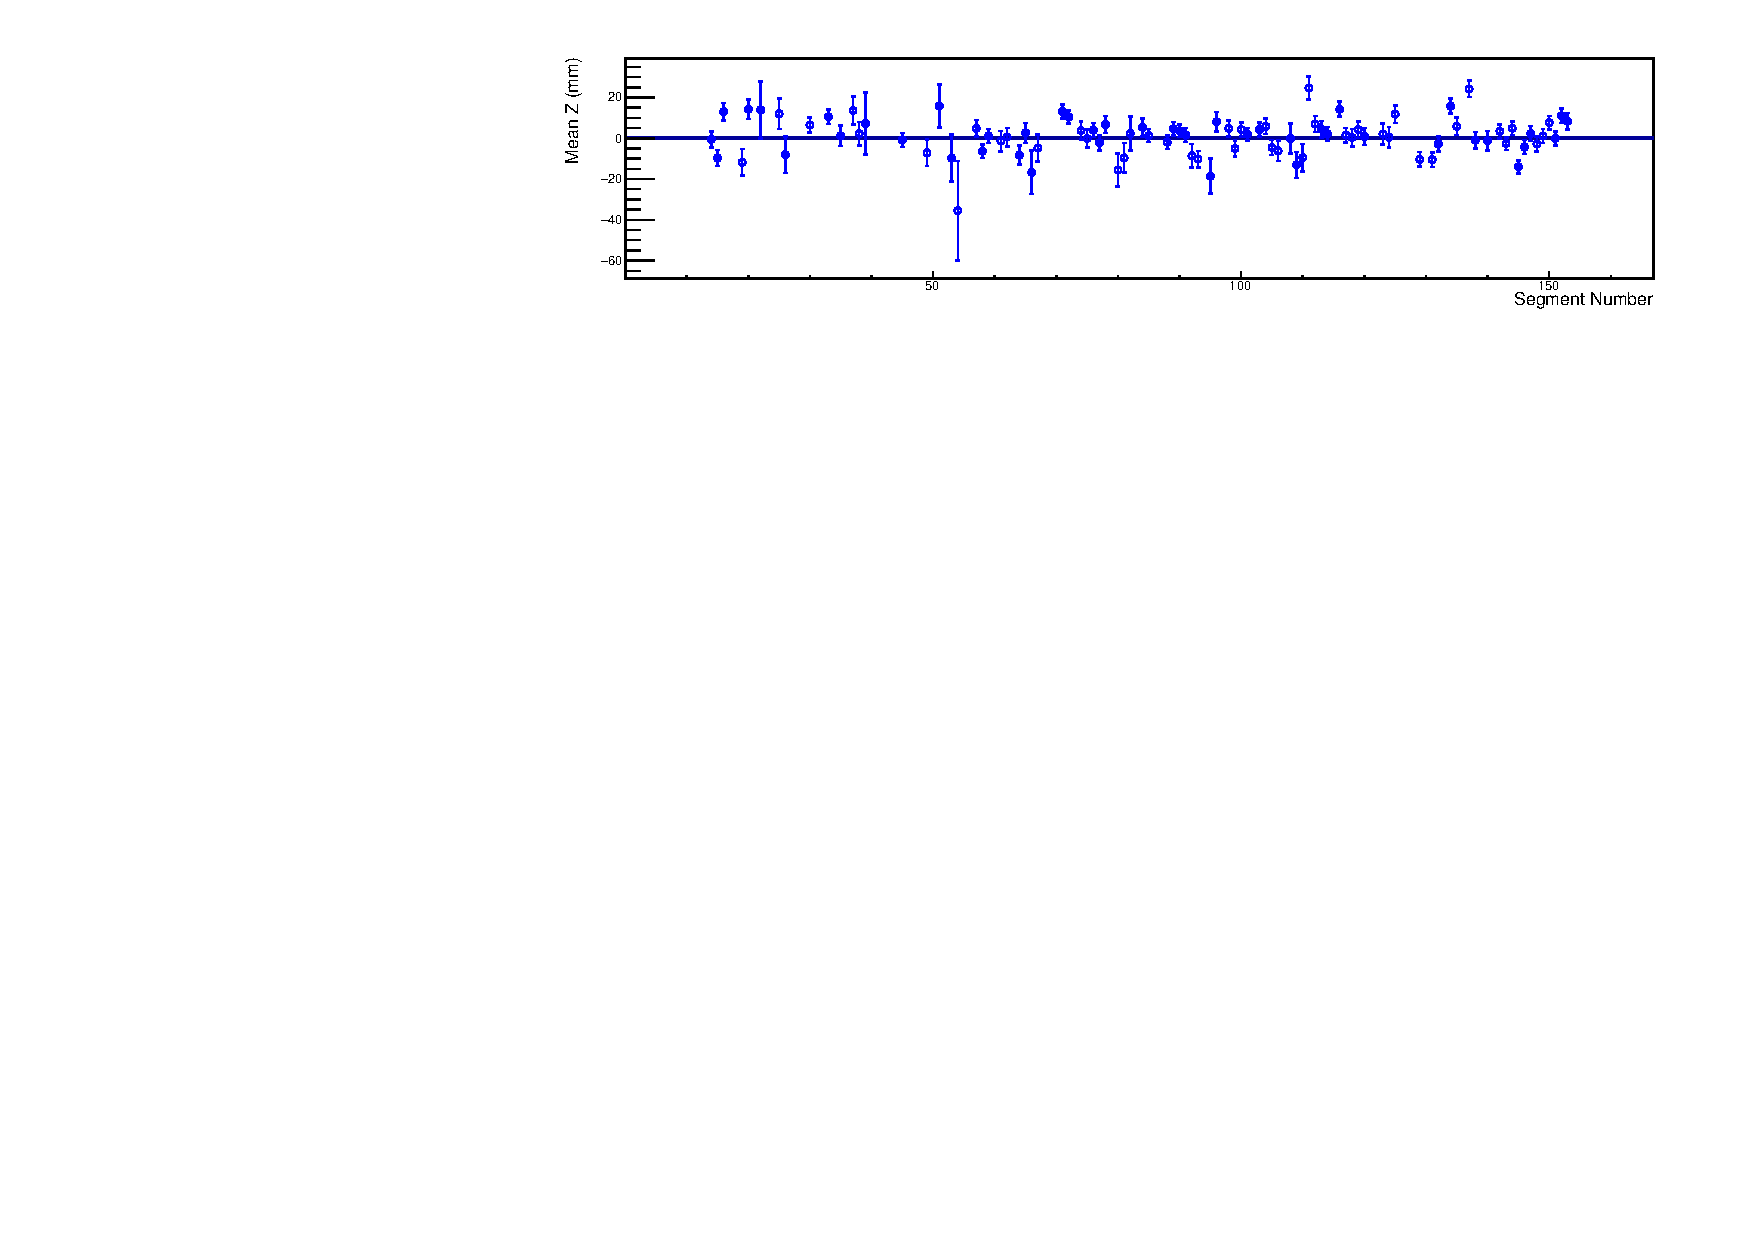
\includegraphics[width=1.05\textwidth]{figures/PubBiPo214meanZvsCell.pdf}
	\caption{\label{fig:meanZvsCell214}Mean of Z-position distribution of Po-214 alphas versus segment. The values are distributions averages and the error bars are the RMS of the distribution. The weighted average mean Z-position is 1.94$\pm$0.43~mm and $\chi^2$/NDF=289/90.}
\end{figure}
\clearpage
\newpage
%------------------------------
\subsection{Energy versus time plots}
\begin{figure}[!h]
\centering
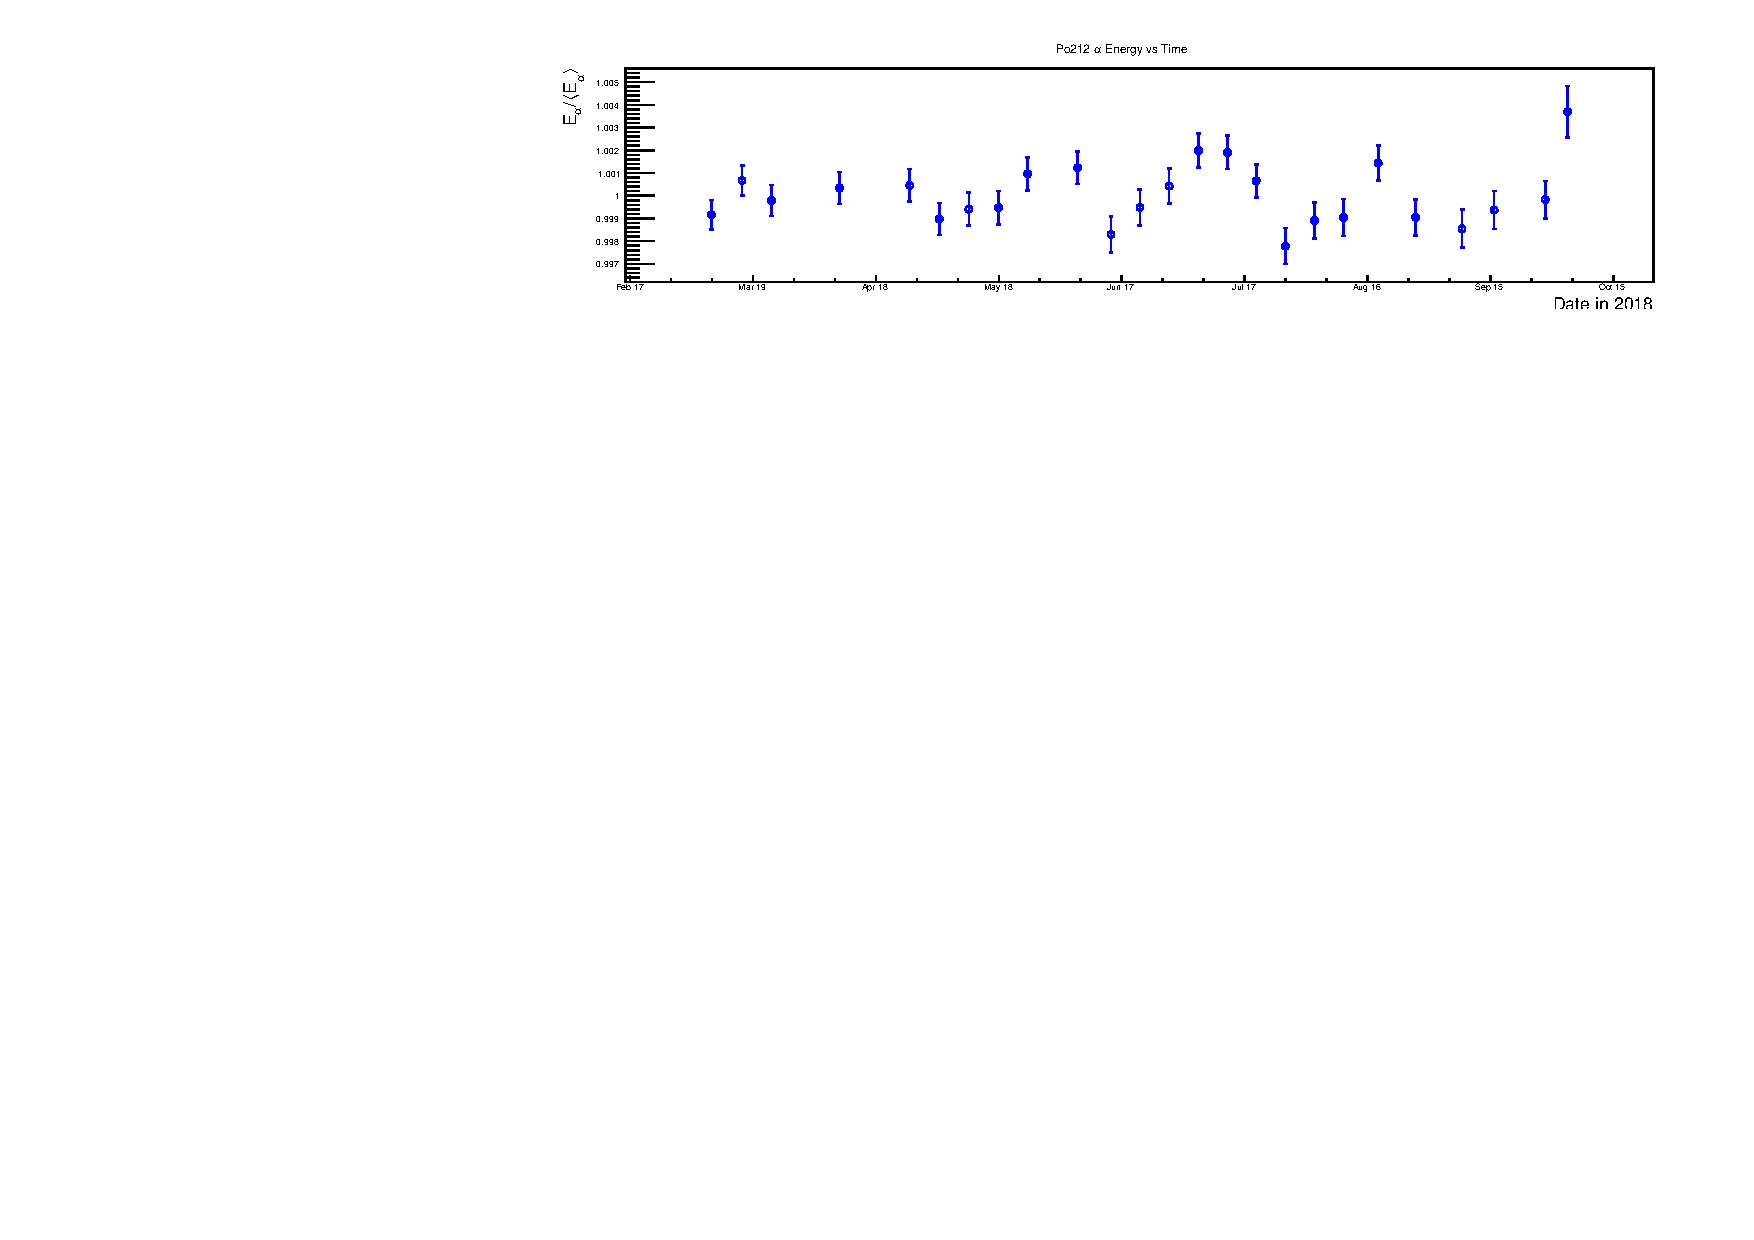
\includegraphics[width=1.05\textwidth]{figures/PubBiPo212EvsT.pdf}
\caption{\label{fig:EvsT212}Po-212 detector averaged alpha energy versus time. The value is the mean of a Gaussian fit to the alpha energy peak and the error bar is the 1$\sigma$ width. Energy is normalized to the segment error-weighted average to highlight variations. Un-normalized weighted average energy is 1.05924$\pm$0.00016~MeV and $\chi^2$/NDF=62/24. }
\end{figure}
\begin{figure}[!h]
\centering
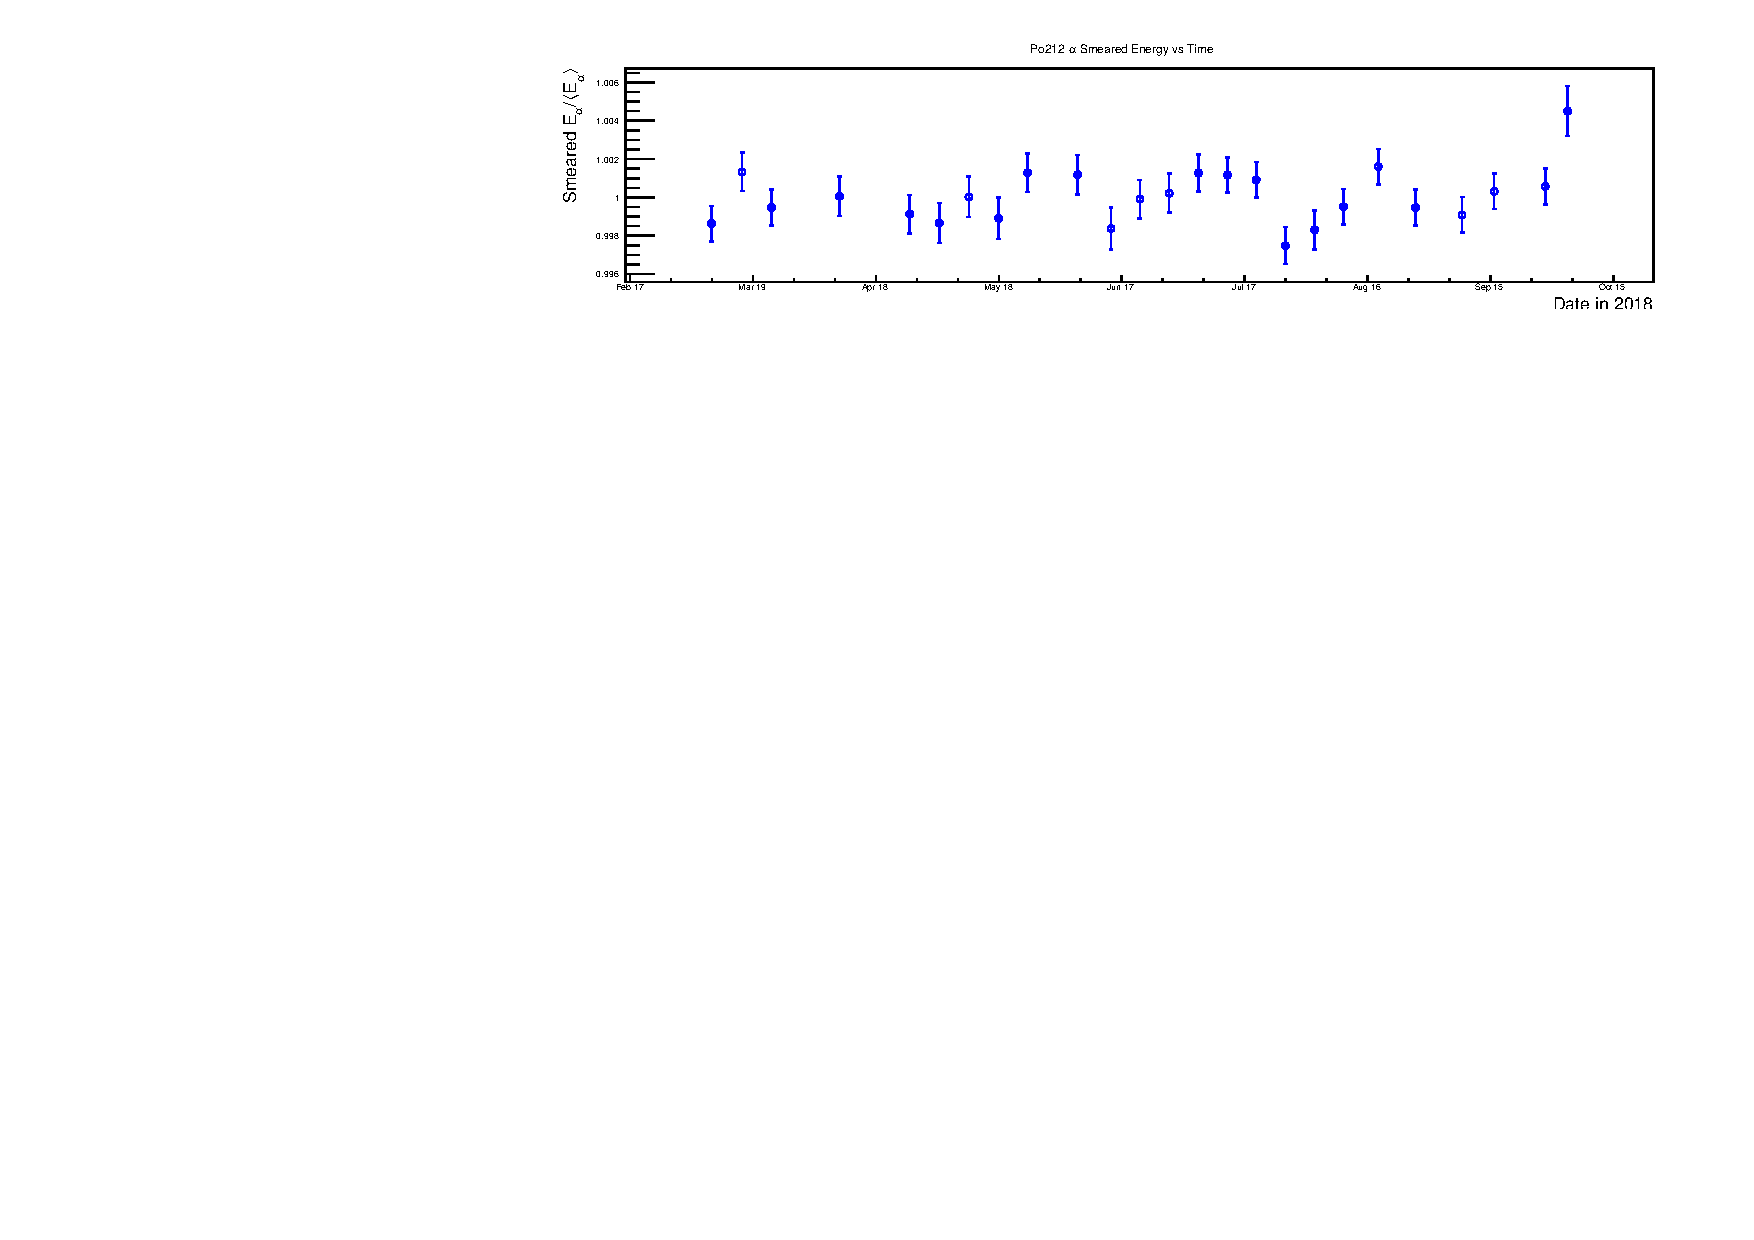
\includegraphics[width=1.05\textwidth]{figures/PubBiPo212EsmearvsT.pdf}
\caption{\label{fig:EsmearvsT212}Po-212 detector-averaged {\bf smeared} alpha energy versus time. The value is the mean of a Gaussian fit to the alpha energy peak and the error bar is the 1$\sigma$ width. Energy is normalized to the segment error-weighted average to highlight variations. Un-normalized weighted average energy is 1.05899$\pm$0.00021~MeV and $\chi^2$/NDF=44/24. }
\end{figure}
\FloatBarrier
\newpage
\begin{figure}[!h]
\centering
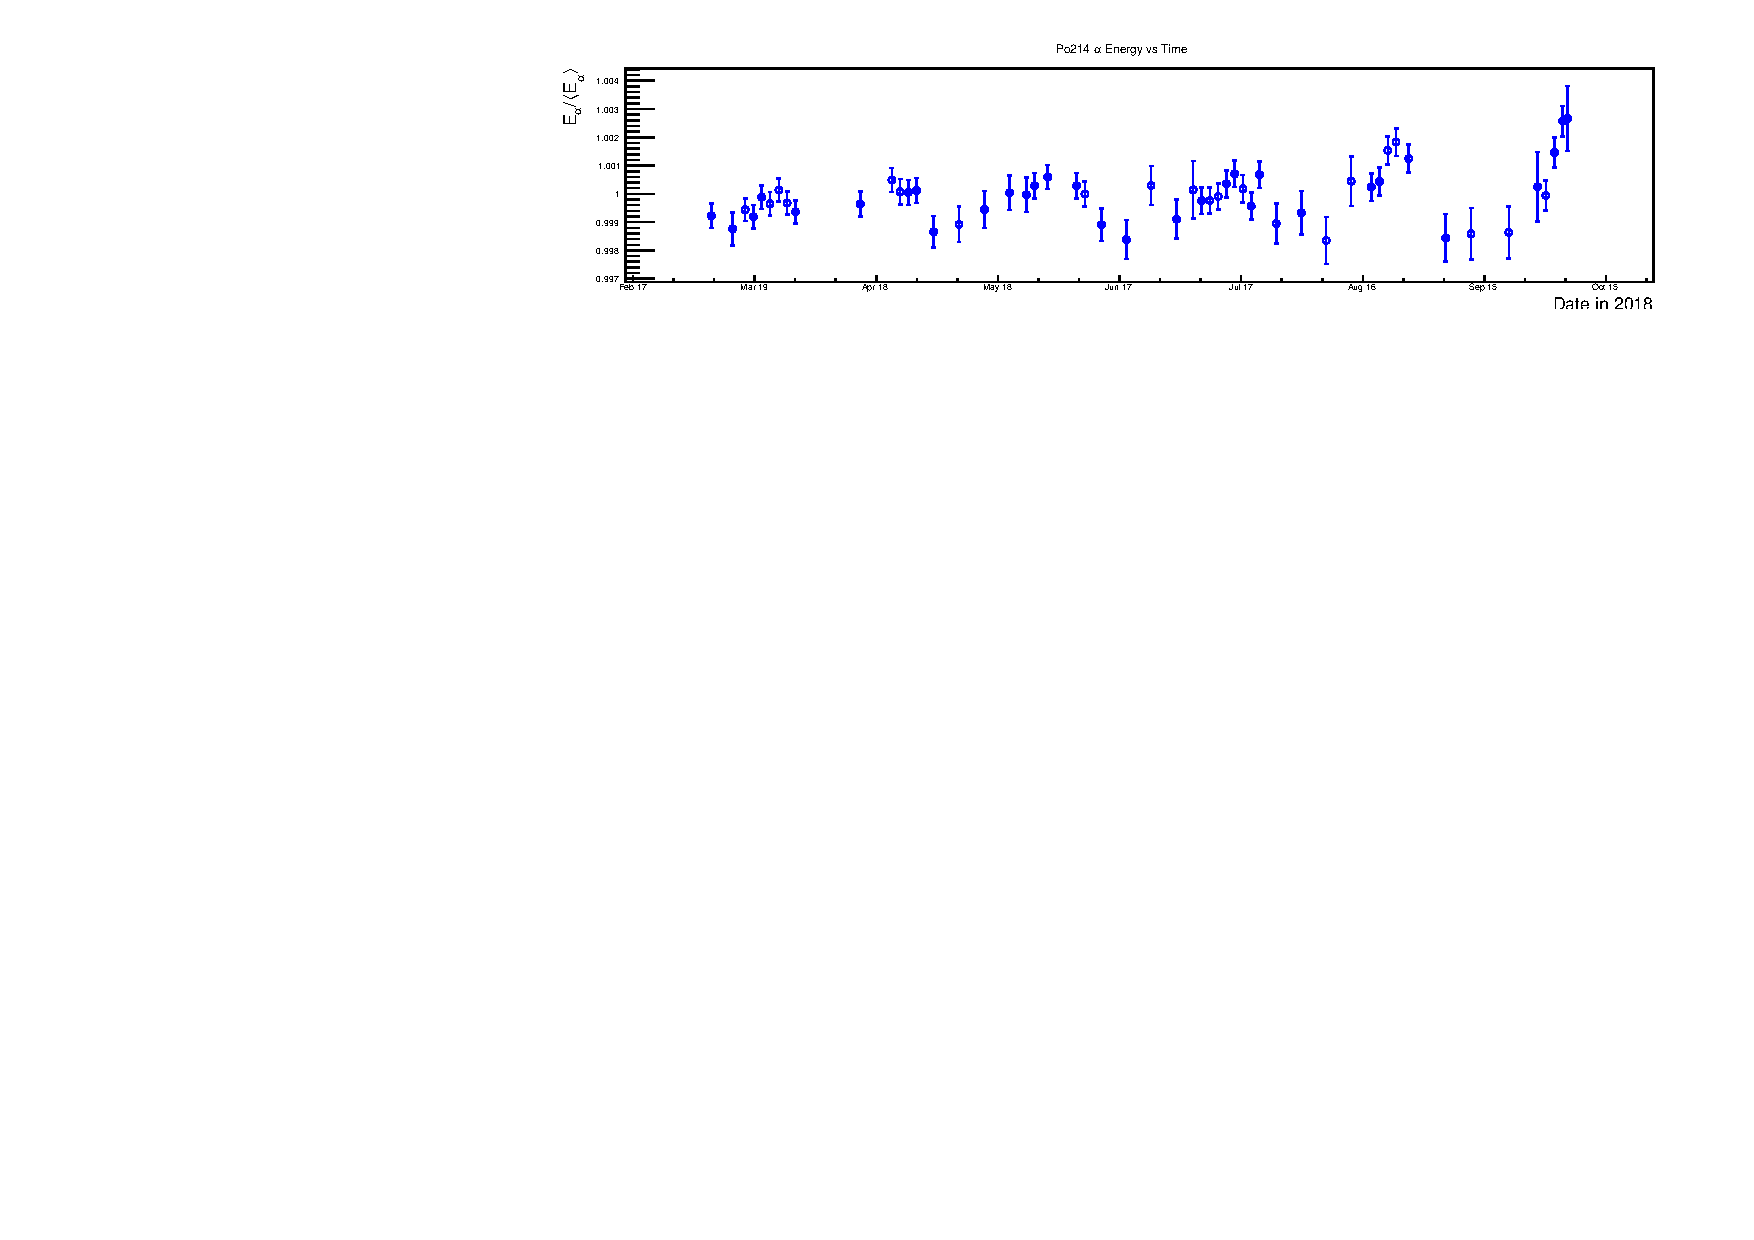
\includegraphics[width=1.05\textwidth]{figures/PubBiPo214EvsT.pdf}
\caption{\label{fig:EvsT214}Po-214 detector-averaged alpha energy versus time. The value is the mean of a Gaussian fit to the alpha energy peak and the error bar is the 1$\sigma$ width. Energy is normalized to the segment error-weighted average to highlight variations. Un-normalized weighted average energy is 0.84147$\pm$0.00006~MeV and $\chi^2$/NDF=131/52. Data points during reactor on periods include 3 times more data to reduce error bar size since accidental backgrounds for this BiPo-214 decay process are much larger. The BiPo-212 decay has almost no accidental backgrounds due to the relatively short lifetime of Po-212 (299~ns).}
\end{figure}
\begin{figure}[!h]
\centering
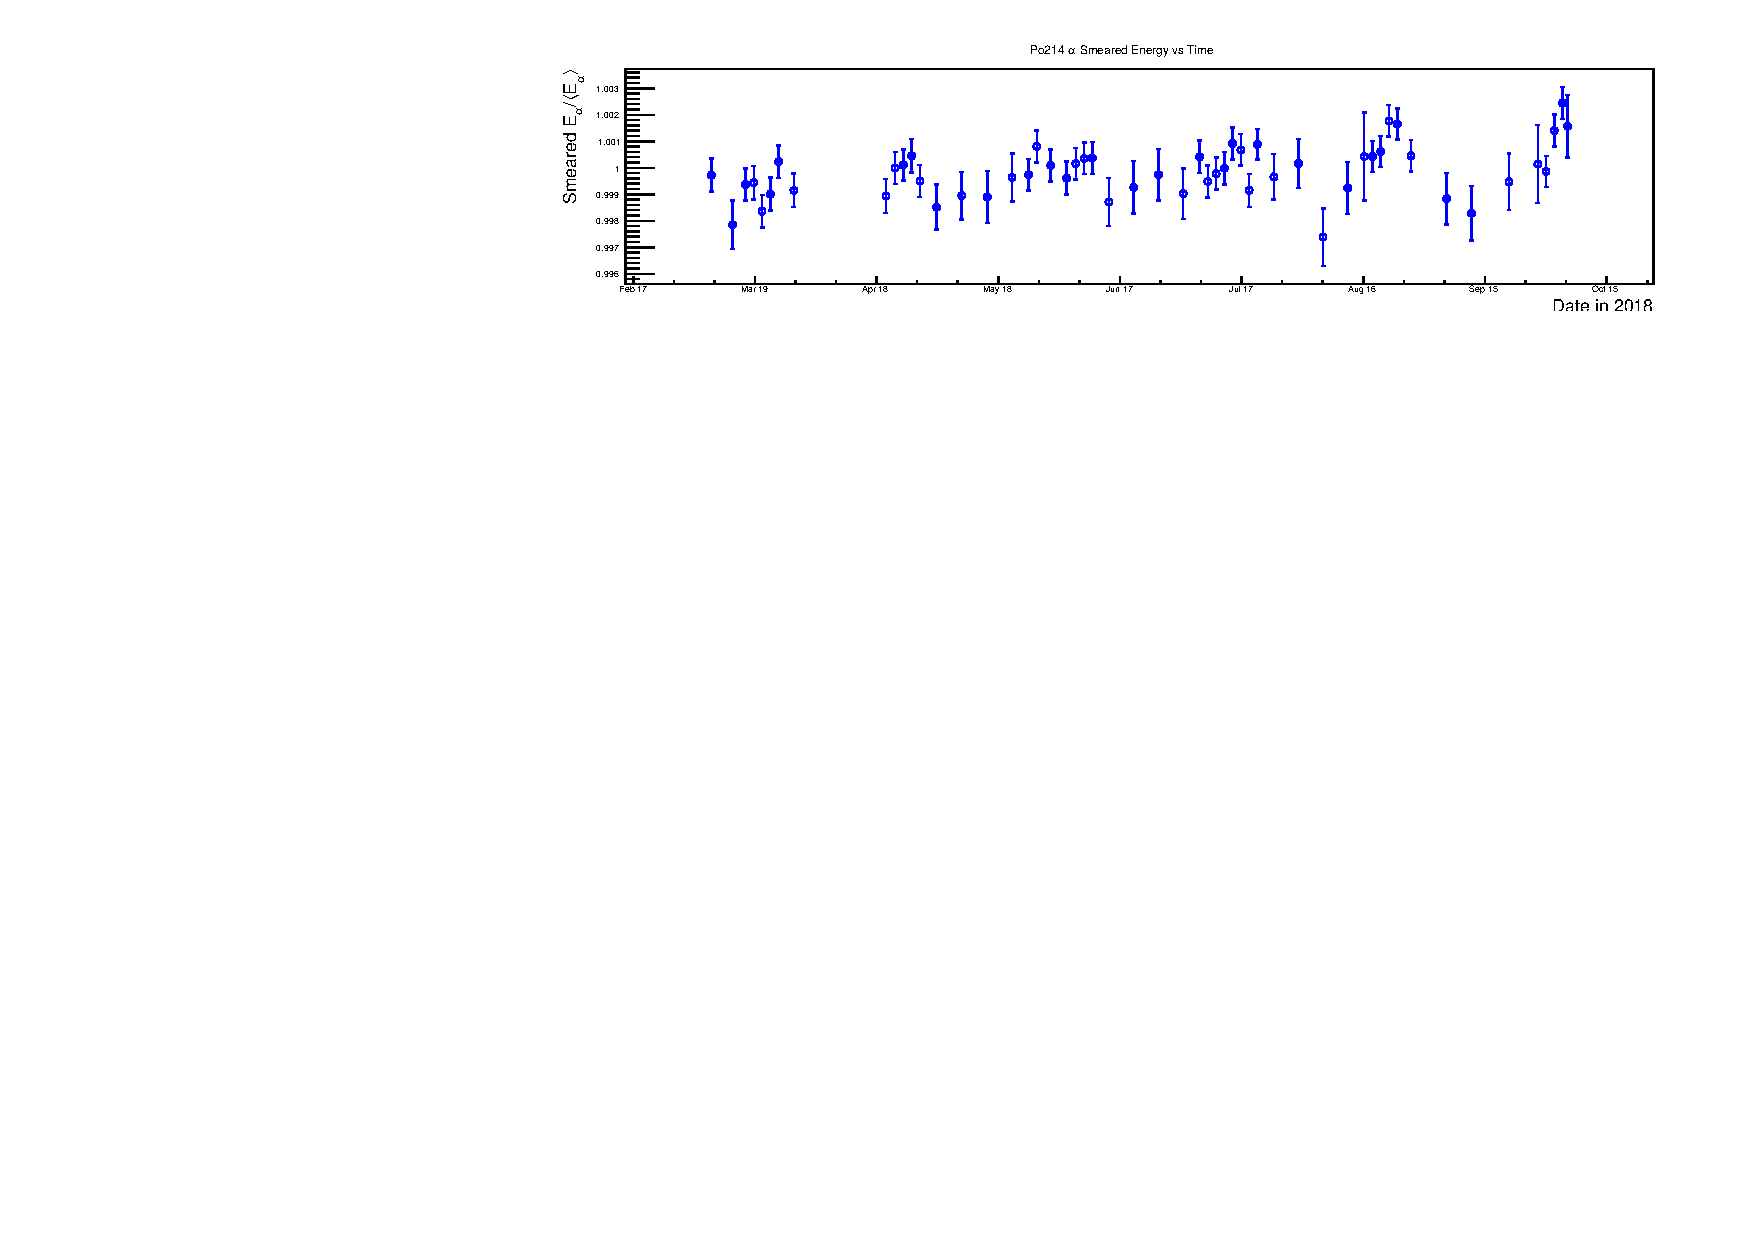
\includegraphics[width=1.05\textwidth]{figures/PubBiPo214EsmearvsT.pdf}
\caption{\label{fig:EsmearvsT214}Po-214 detector-averaged {\bf smeared} alpha energy versus time. The value is the mean of a Gaussian fit to the alpha energy peak and the error bar is the 1$\sigma$ width. Energy is normalized to the segment error-weighted average to highlight variations. Un-normalized weighted average energy is 0.84089$\pm$0.00008~MeV and $\chi^2$/NDF=97/52. Data points during reactor on periods include 3 times more data to reduce error bar size since accidental backgrounds for this BiPo-214 decay process are much larger. The BiPo-212 decay has almost no accidental backgrounds due to the relatively short lifetime of Po-212 (299~ns).}
\end{figure}
\FloatBarrier
\newpage
%------------------------------
\subsection{Energy resolution versus time plots}
\begin{figure}[!h]
\centering
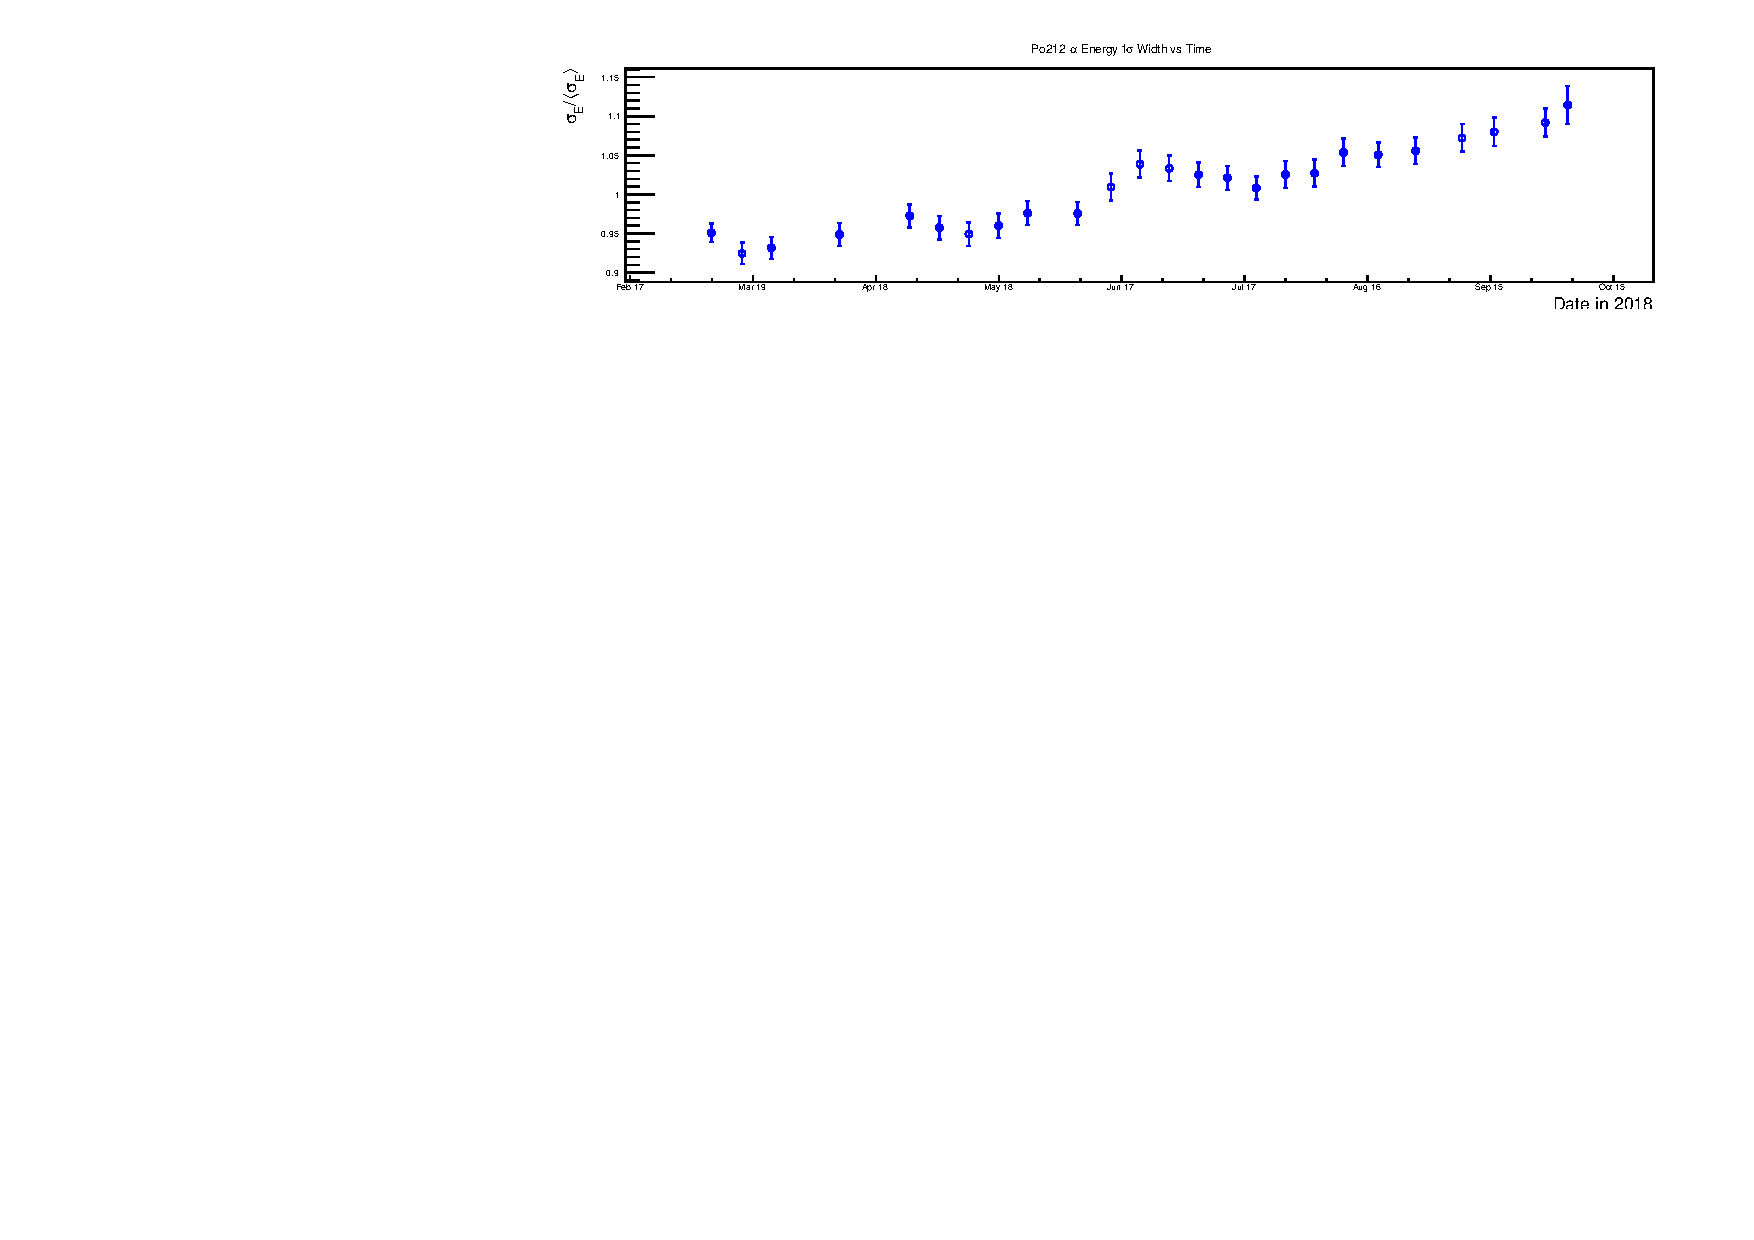
\includegraphics[width=1.05\textwidth]{figures/PubBiPo212EresvsT.pdf}
\caption{\label{fig:EresvsT212}Detector averaged energy resolution versus time using the alpha from Po-212 decay. The values are the 1$\sigma$ widths of a Gaussian fits to the alpha energy peaks and the error bars are the error on these values from the fit. Values are normalized to the segment error-weighted average to highlight variations. Un-normalized weighted average energy width is 0.04976$\pm$0.00016~MeV and $\chi^2$/NDF=252/24.}
\end{figure}
\begin{figure}[!h]
\centering
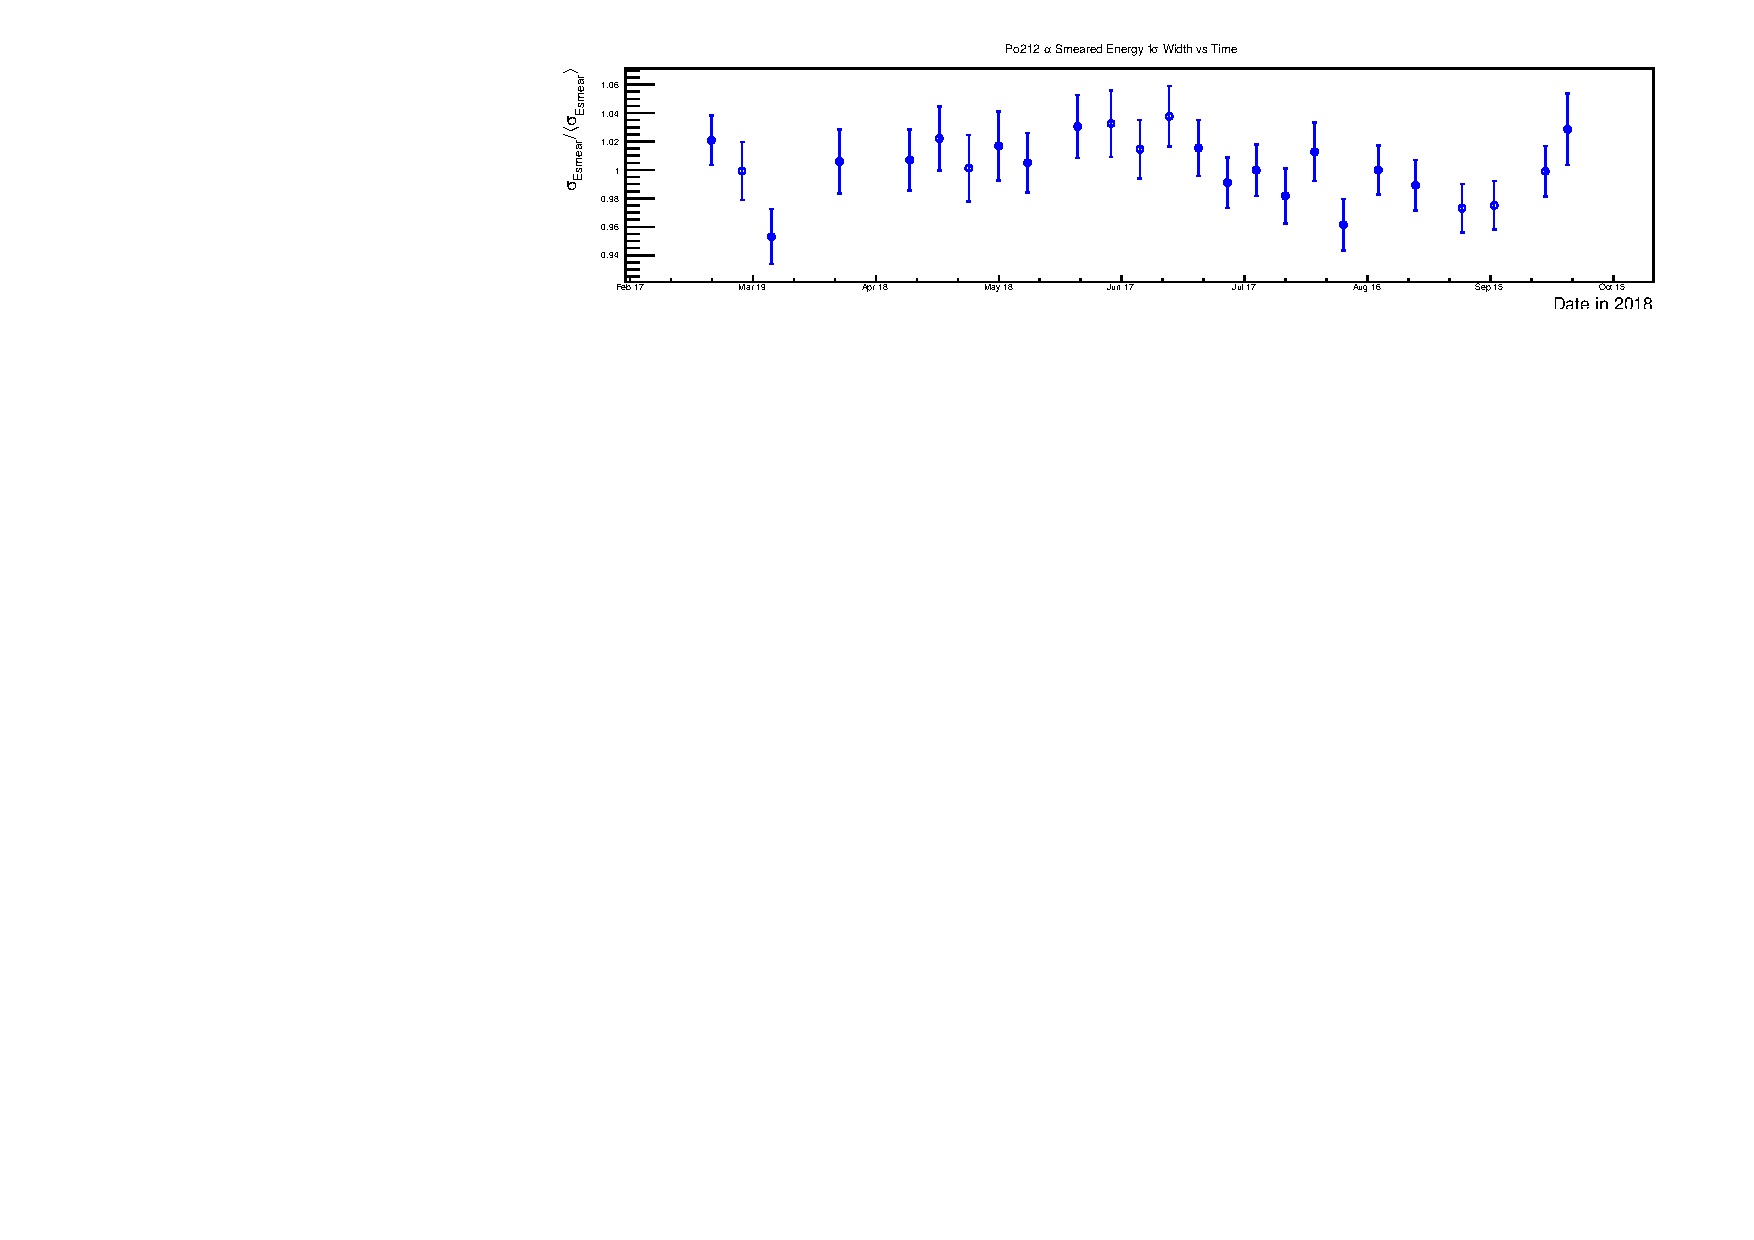
\includegraphics[width=1.05\textwidth]{figures/PubBiPo212EsmearresvsT.pdf}
\caption{\label{fig:EsmearresvsT212}Detector averaged {\bf smeared} energy resolution versus time using the alpha from Po-212 decay. The values are the 1$\sigma$ widths of a Gaussian fits to the alpha energy peaks and the error bars are the error on these values from the fit. Values are normalized to the segment error-weighted average to highlight variations. Un-normalized weighted average energy width is 0.05839$\pm$0.00023~MeV and $\chi^2$/NDF=29/24.}
\end{figure}
\clearpage
\newpage
\begin{figure}[!h]
\centering
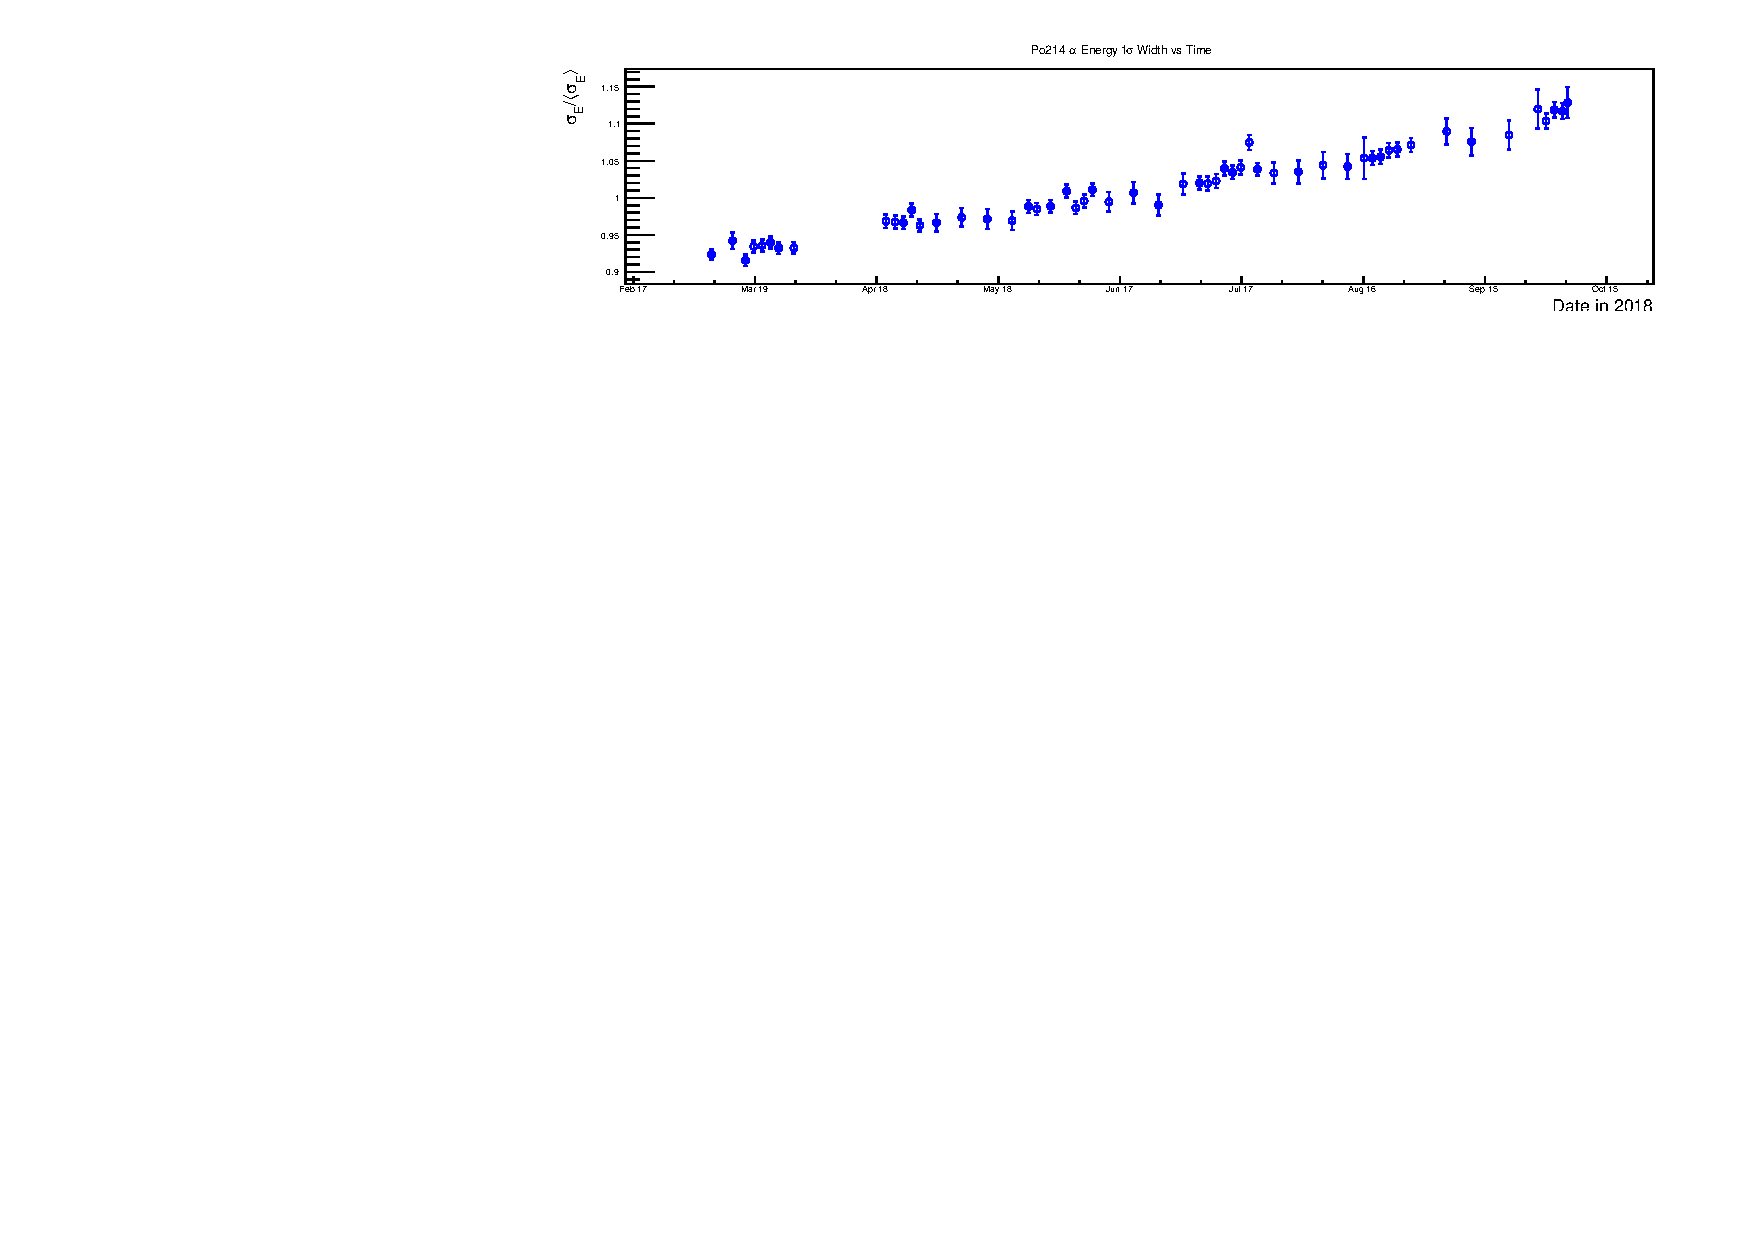
\includegraphics[width=1.05\textwidth]{figures/PubBiPo214EresvsT.pdf}
\caption{\label{fig:EresvsT214}Detector-averaged energy resolution versus time using the alpha from Po-214 decay. The values are the 1$\sigma$ widths of a Gaussian fits to the alpha energy peaks and the error bars are the error on these values from the fit. Values are normalized to the segment error-weighted average to highlight variations. Un-normalized weighted average energy width is 0.04314$\pm$0.00006~MeV and $\chi^2$/NDF=1613/52.}
\end{figure}
\begin{figure}[!h]
\centering
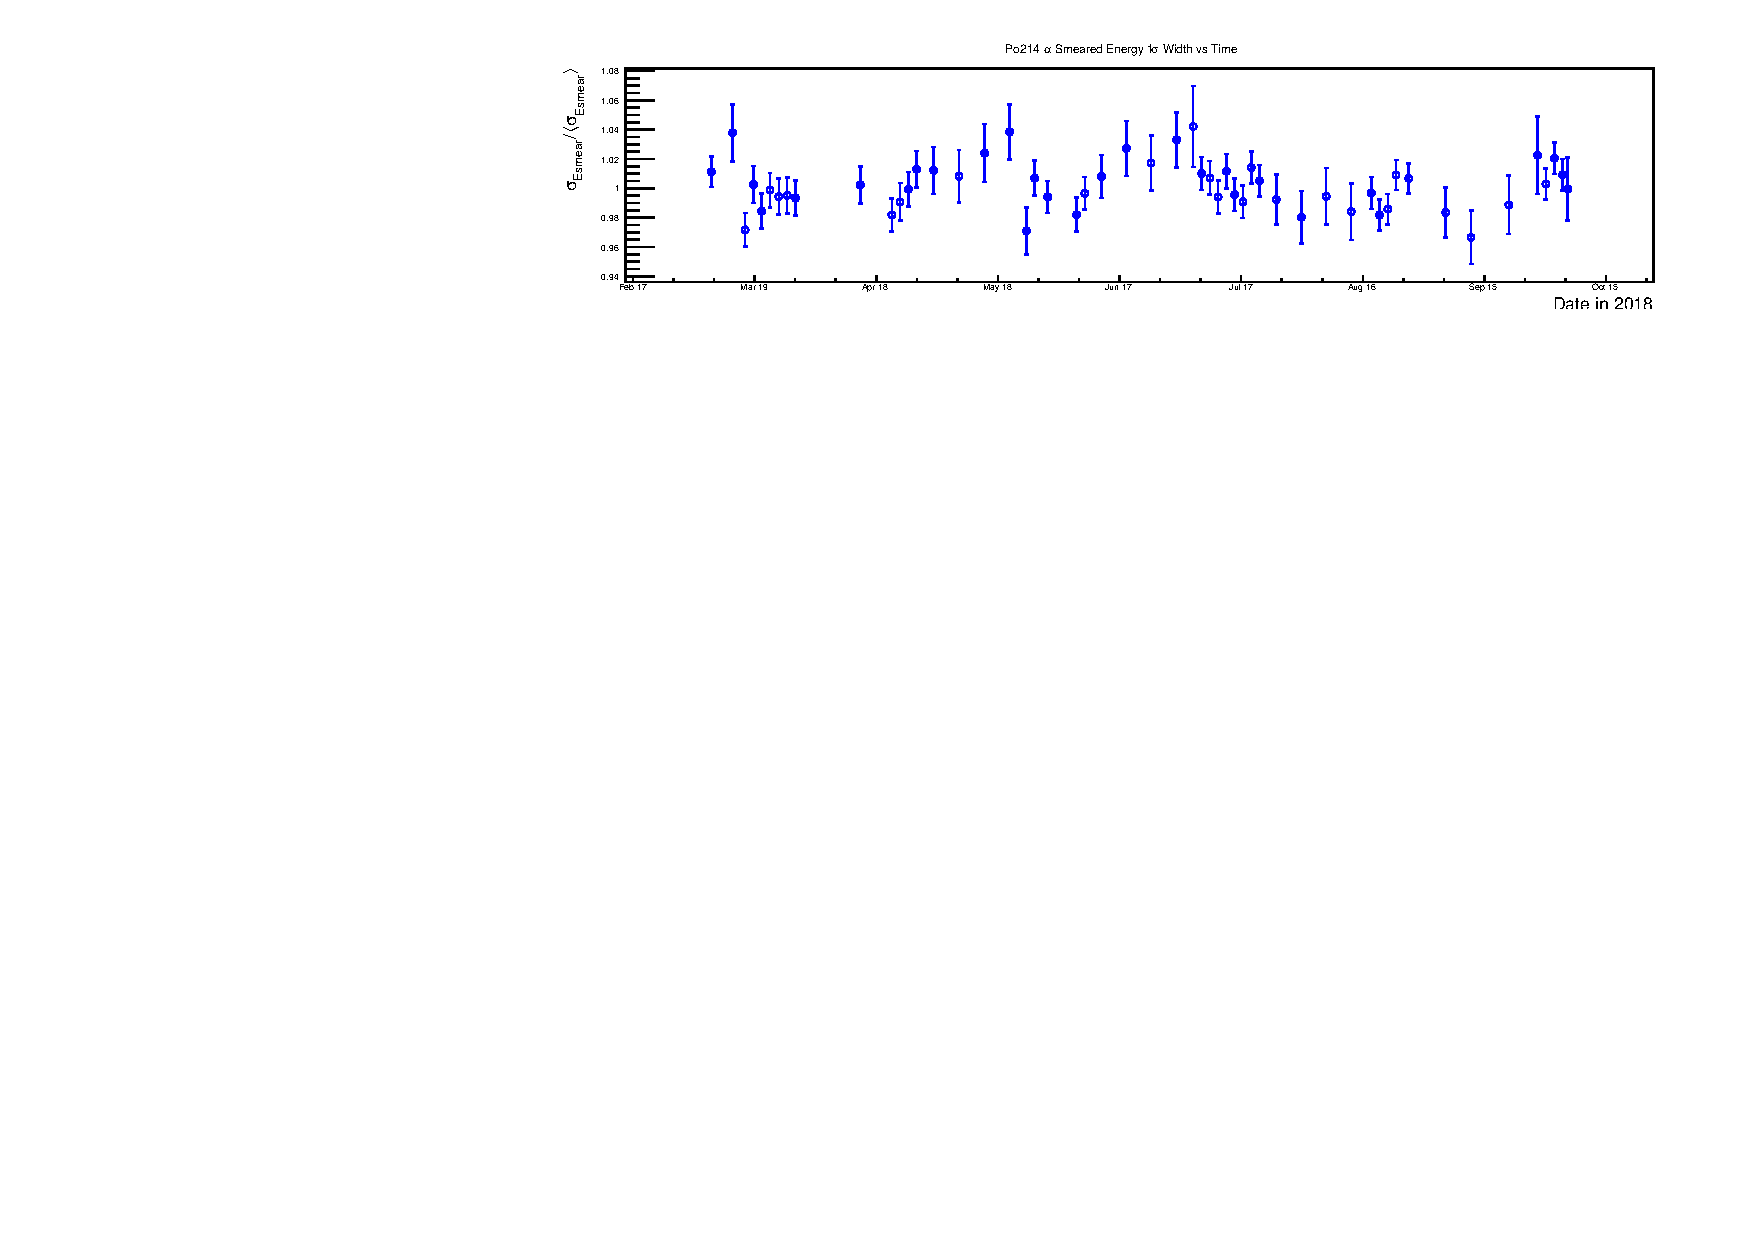
\includegraphics[width=1.05\textwidth]{figures/PubBiPo214EsmearresvsT.pdf}
\caption{\label{fig:EsmearresvsT214}Detector-averaged {\bf smeared} energy resolution versus time using the alpha from Po-214 decay. The values are the 1$\sigma$ widths of a Gaussian fits to the alpha energy peaks and the error bars are the error on these values from the fit. Values are normalized to the segment error-weighted average to highlight variations. Un-normalized weighted average energy width is 0.05187$\pm$0.00009~MeV and $\chi^2$/NDF=63/52.}
\end{figure}
\clearpage
\newpage
%------------------------------
\subsection{Z-distribution RMS width versus time plots}
\begin{figure}[!h]
\centering
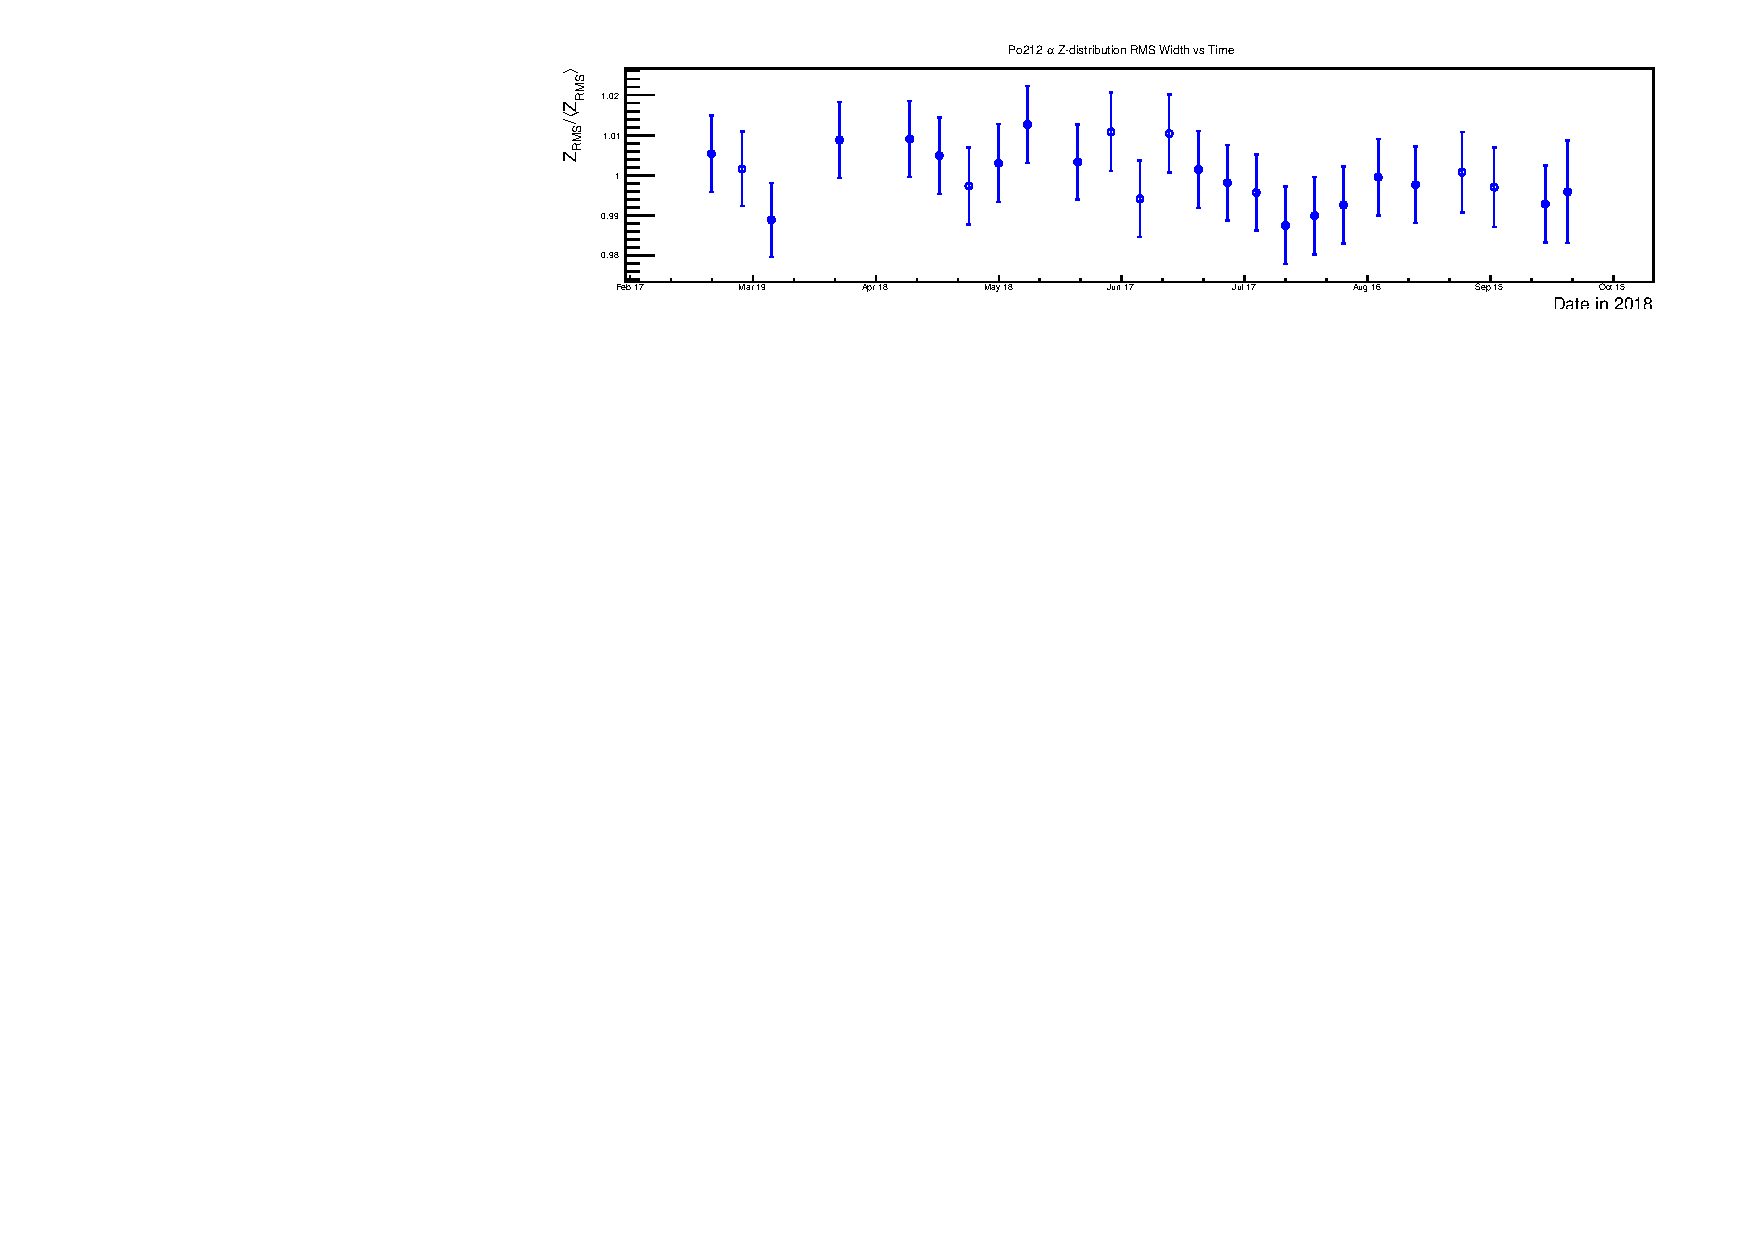
\includegraphics[width=1.05\textwidth]{figures/PubBiPo212ZrmsvsT.pdf}
\caption{\label{fig:ZRMSvsT212}RMS width of Z-distribution of Po-212 alphas versus time. The error bars are the errors assigned by ROOT to the RMS values of the histograms. Values are normalized to the segment error-weighted average to highlight variations. Un-normalized weighted average Z$_{RMS}$ width is 348.7$\pm$0.7~mm and the $\chi^2$/NDF=13/24. }
\end{figure}
\begin{figure}[!h]
\centering
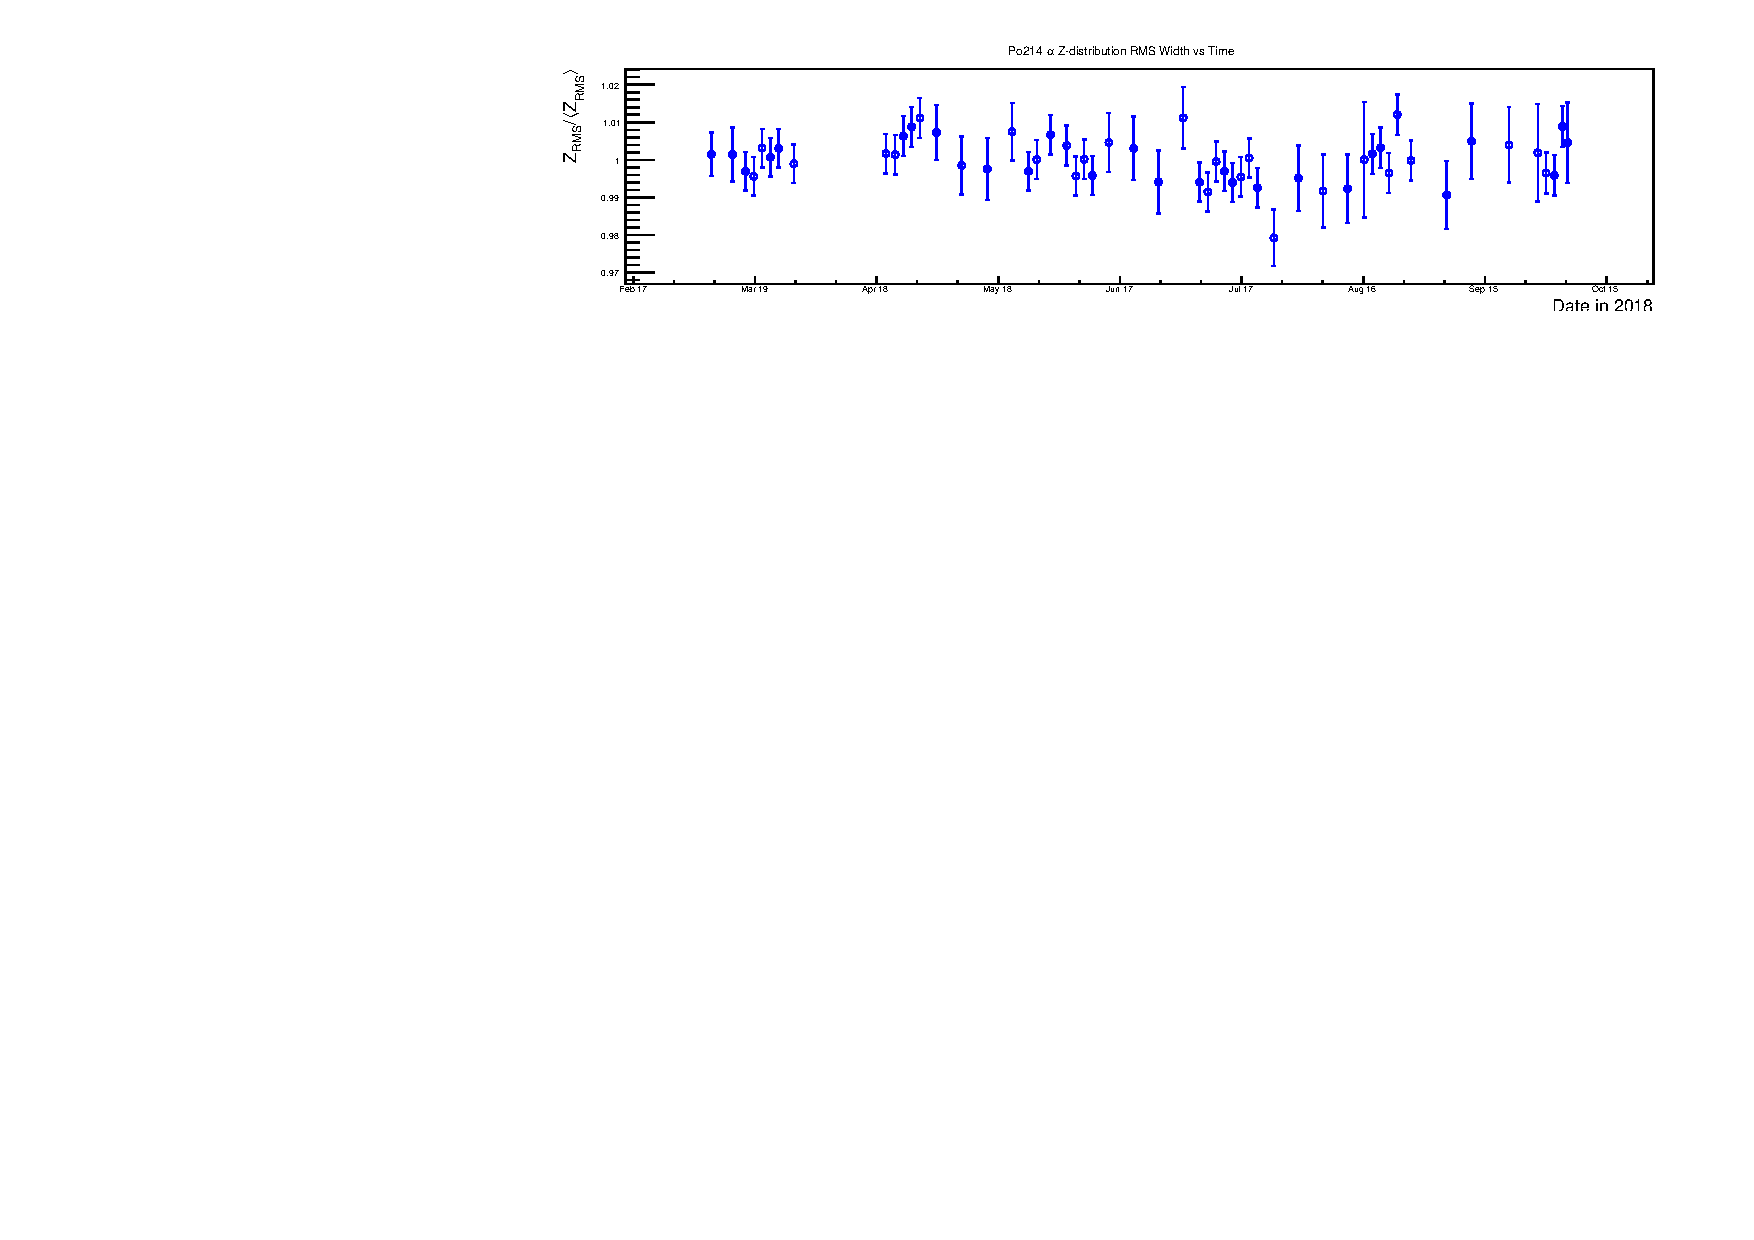
\includegraphics[width=1.05\textwidth]{figures/PubBiPo214ZrmsvsT.pdf}
\caption{\label{fig:ZRMSvsT214}RMS width of Z-distribution of Po-214 alphas versus Time. The error bars are the errors assigned by ROOT to the RMS values of the histograms. Values are normalized to the segment error-weighted average to highlight variations. Un-normalized weighted average Z$_{RMS}$ width is 347.6$\pm$0.3~mm and the $\chi^2$/NDF=55/52}
\end{figure}
\newpage
%------------------------------
\subsection{Z-position resolution versus time plots}
\begin{figure}[!h]
\centering
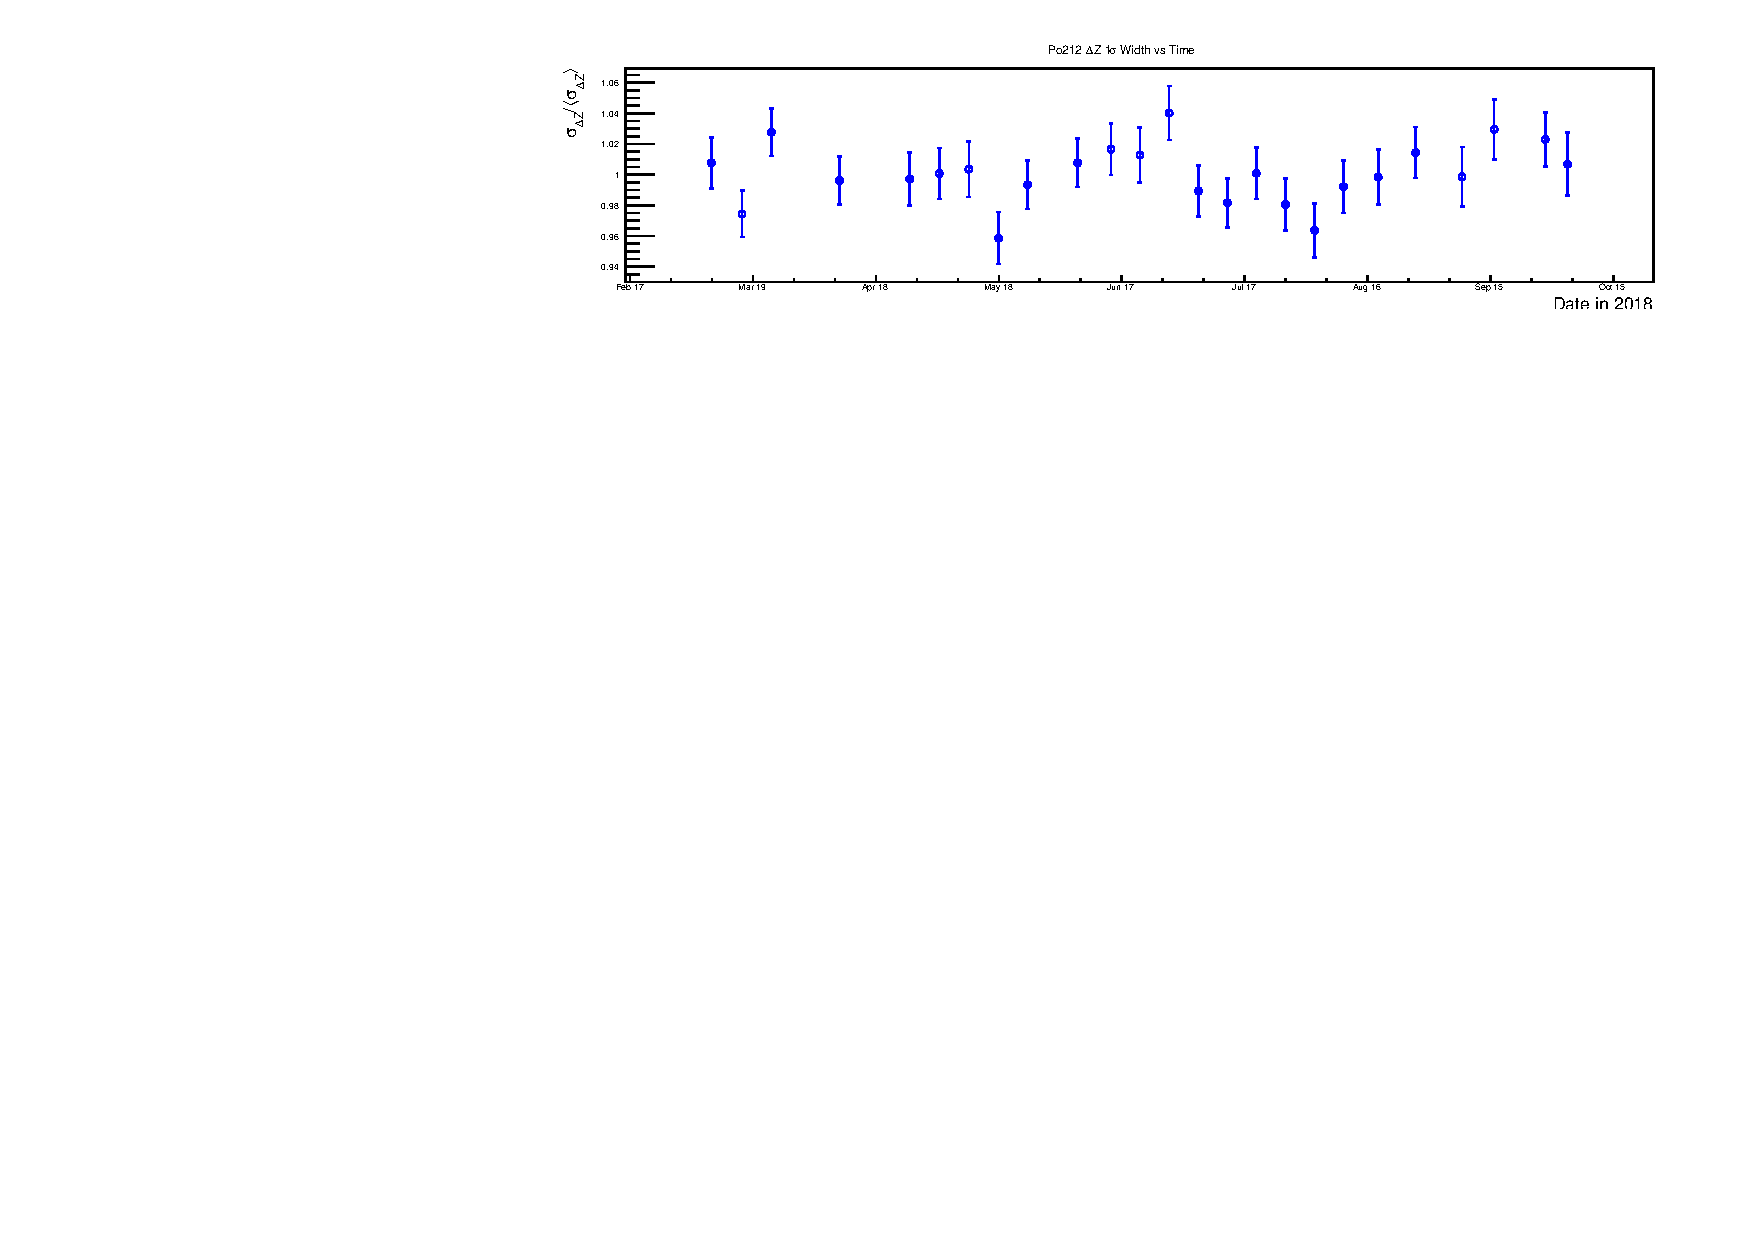
\includegraphics[width=1.05\textwidth]{figures/PubBiPo212ZresvsT.pdf}
\caption{\label{fig:ZresvsT212}Z-position resolution versus time using the beta, alpha from Bi-212, Po-212. The values are the 1$\sigma$ widths of a Gaussian fits to the alpha minus beta Z-distance distributions and the error bars are the error on these values from the fit. Values are normalized to the segment error-weighted average to highlight variations. Un-normalized weighted average $\Delta$Z width is 43.17$\pm$0.15~mm and the $\chi^2$/NDF=32/24.}
\end{figure}
\begin{figure}[!h]
\centering
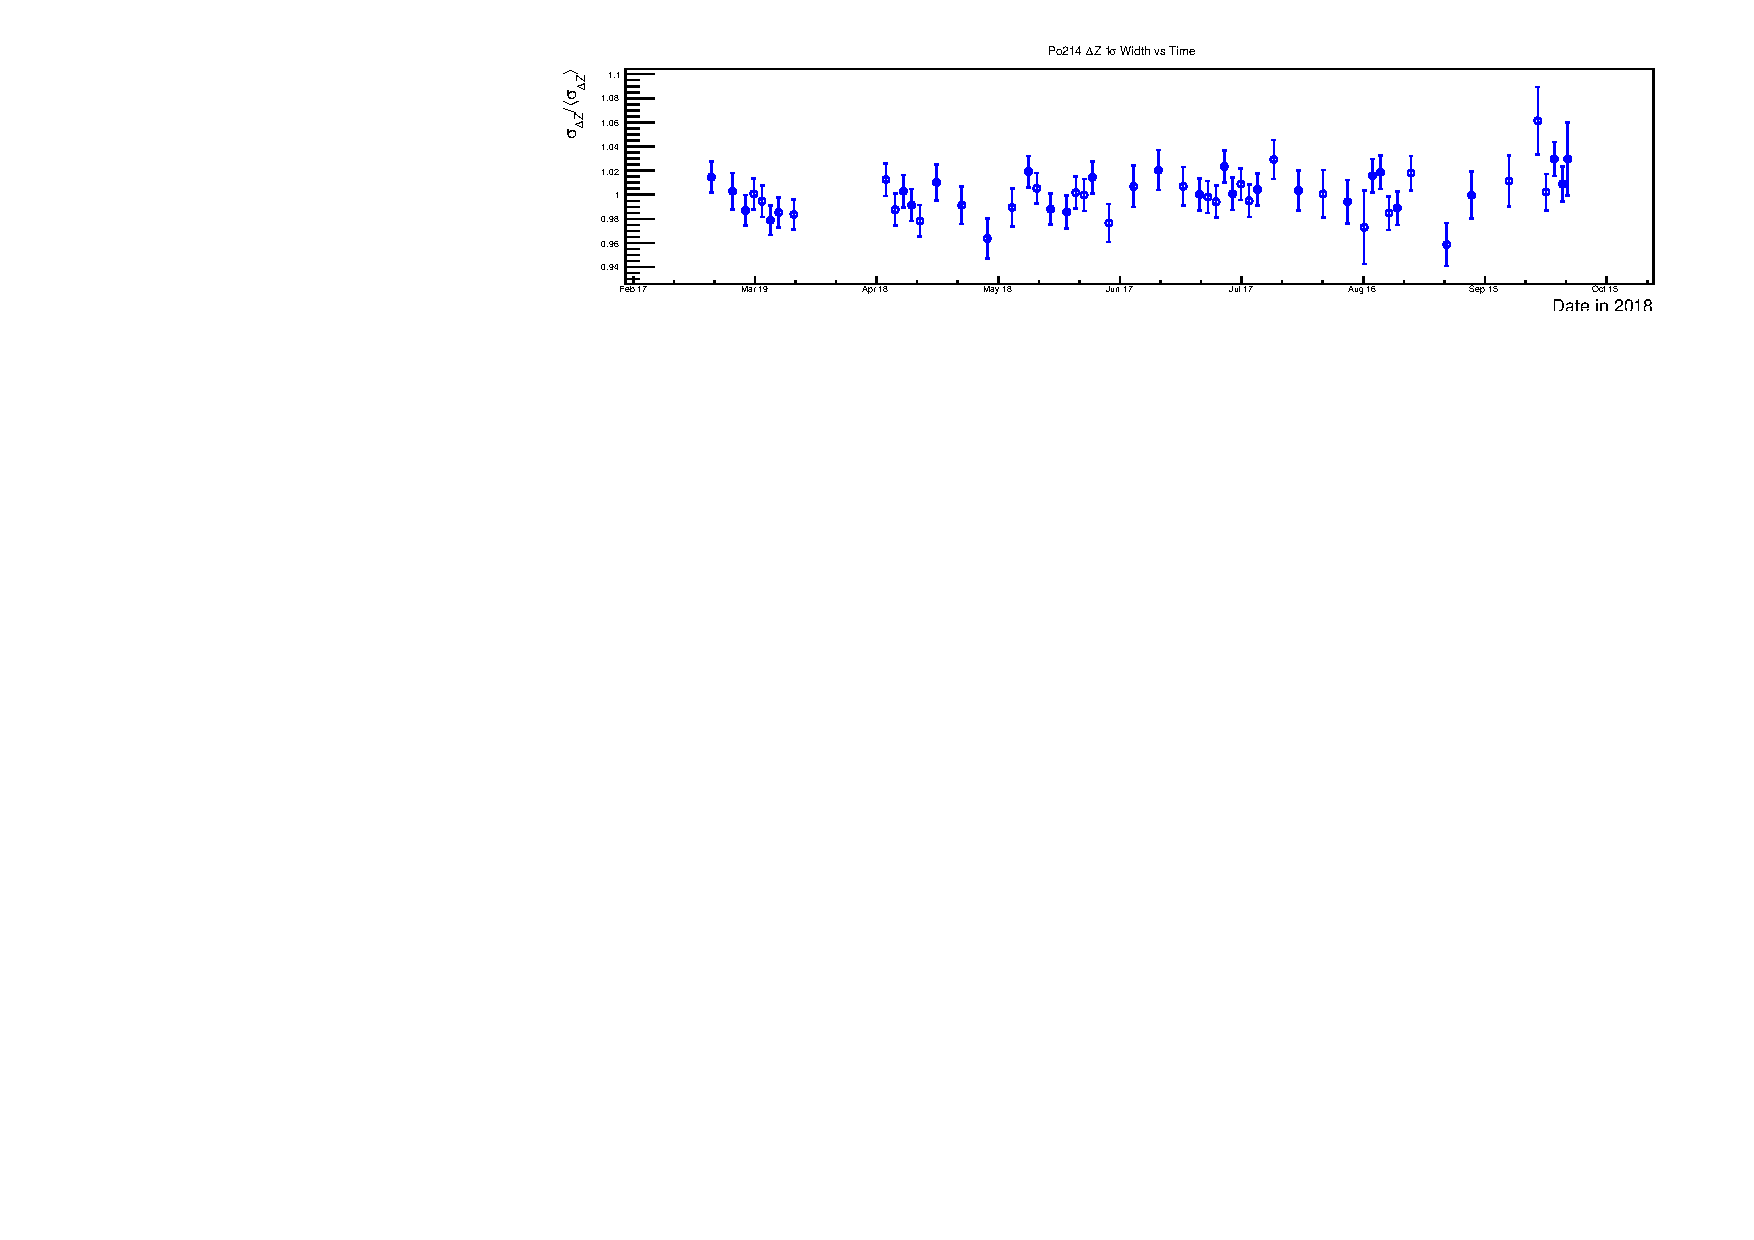
\includegraphics[width=1.05\textwidth]{figures/PubBiPo214ZresvsT.pdf}
\caption{\label{fig:ZresvsT214}Z-position resolution versus time using the beta, alpha from Bi-214, Po-214. The values are the 1$\sigma$ widths of a Gaussian fits to the alpha minus beta Z-distance distributions and the error bars are the error on these values from the fit. Values are normalized to the segment error-weighted average to highlight variations.Un-normalized weighted average $\Delta$Z width is 45.6$\pm$0.1~mm and the $\chi^2$/NDF=55/52. Presumably, the larger width is due to the presence of higher energy gammas accompanying the Po-214 beta decay. Data points during reactor on periods include 3 times more data to reduce error bar size since accidental backgrounds for this BiPo-214 decay process are much larger.}
\end{figure}
\newpage

\newpage
%------------------------------
\subsection{Whole detector alpha energy spectrum}
\begin{figure}[!h]
\centering
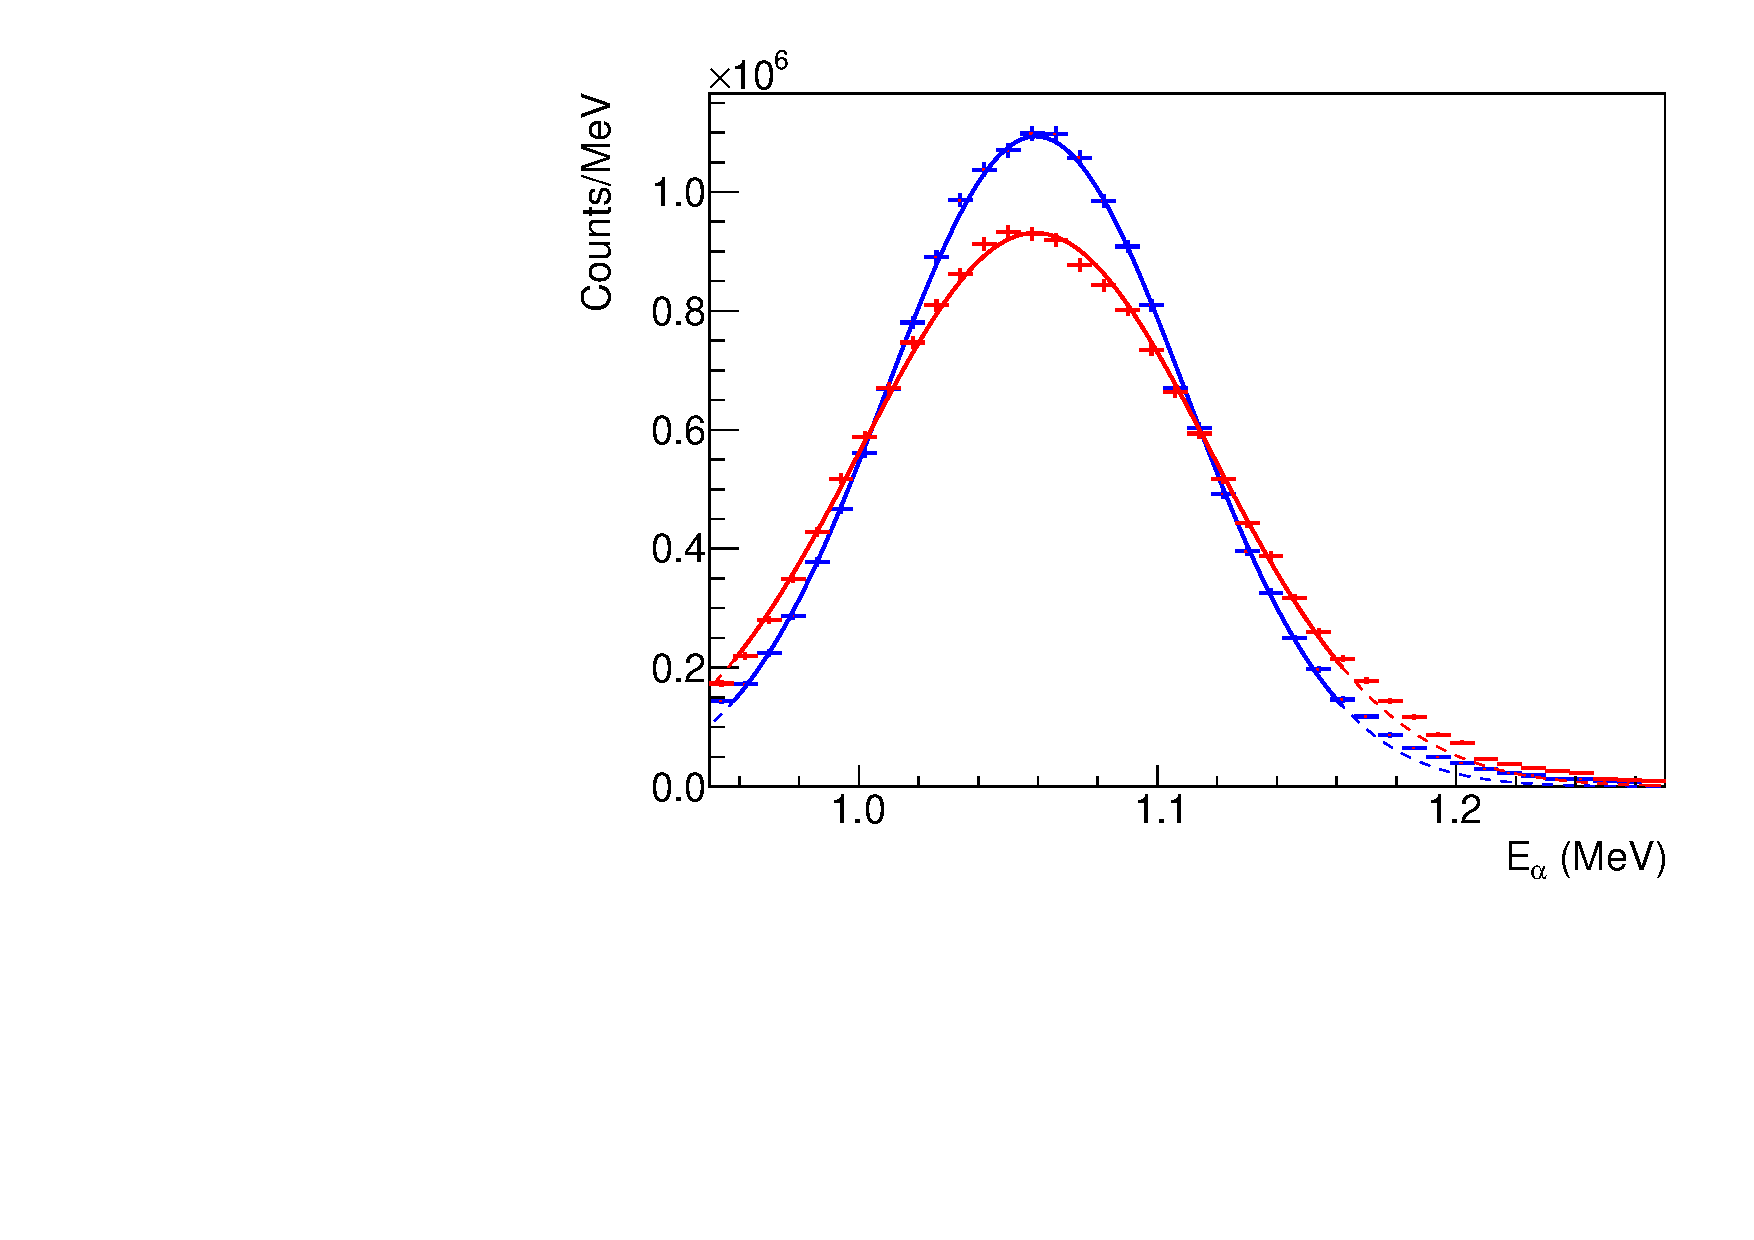
\includegraphics[width=0.56\textwidth]{figures/PubBiPo212AlphaE.pdf}
\caption{\label{fig:AlphaE212}Whole detector Po-212 alpha energy spectrum (blue) and the smeared alpha energy (red). The mean of the unsmeared fit is 1.06494$\pm$0.00014~MeV and the width is 0.05000$\pm$0.00013~MeV. The solid line shows the fit over the range of data included while the dashed line shows what the fit function looks like in the tails outside the fit region. This is an essentially mono-energetic alpha with 8.785~MeV of energy.}
\end{figure}
\begin{figure}[!h]
\centering
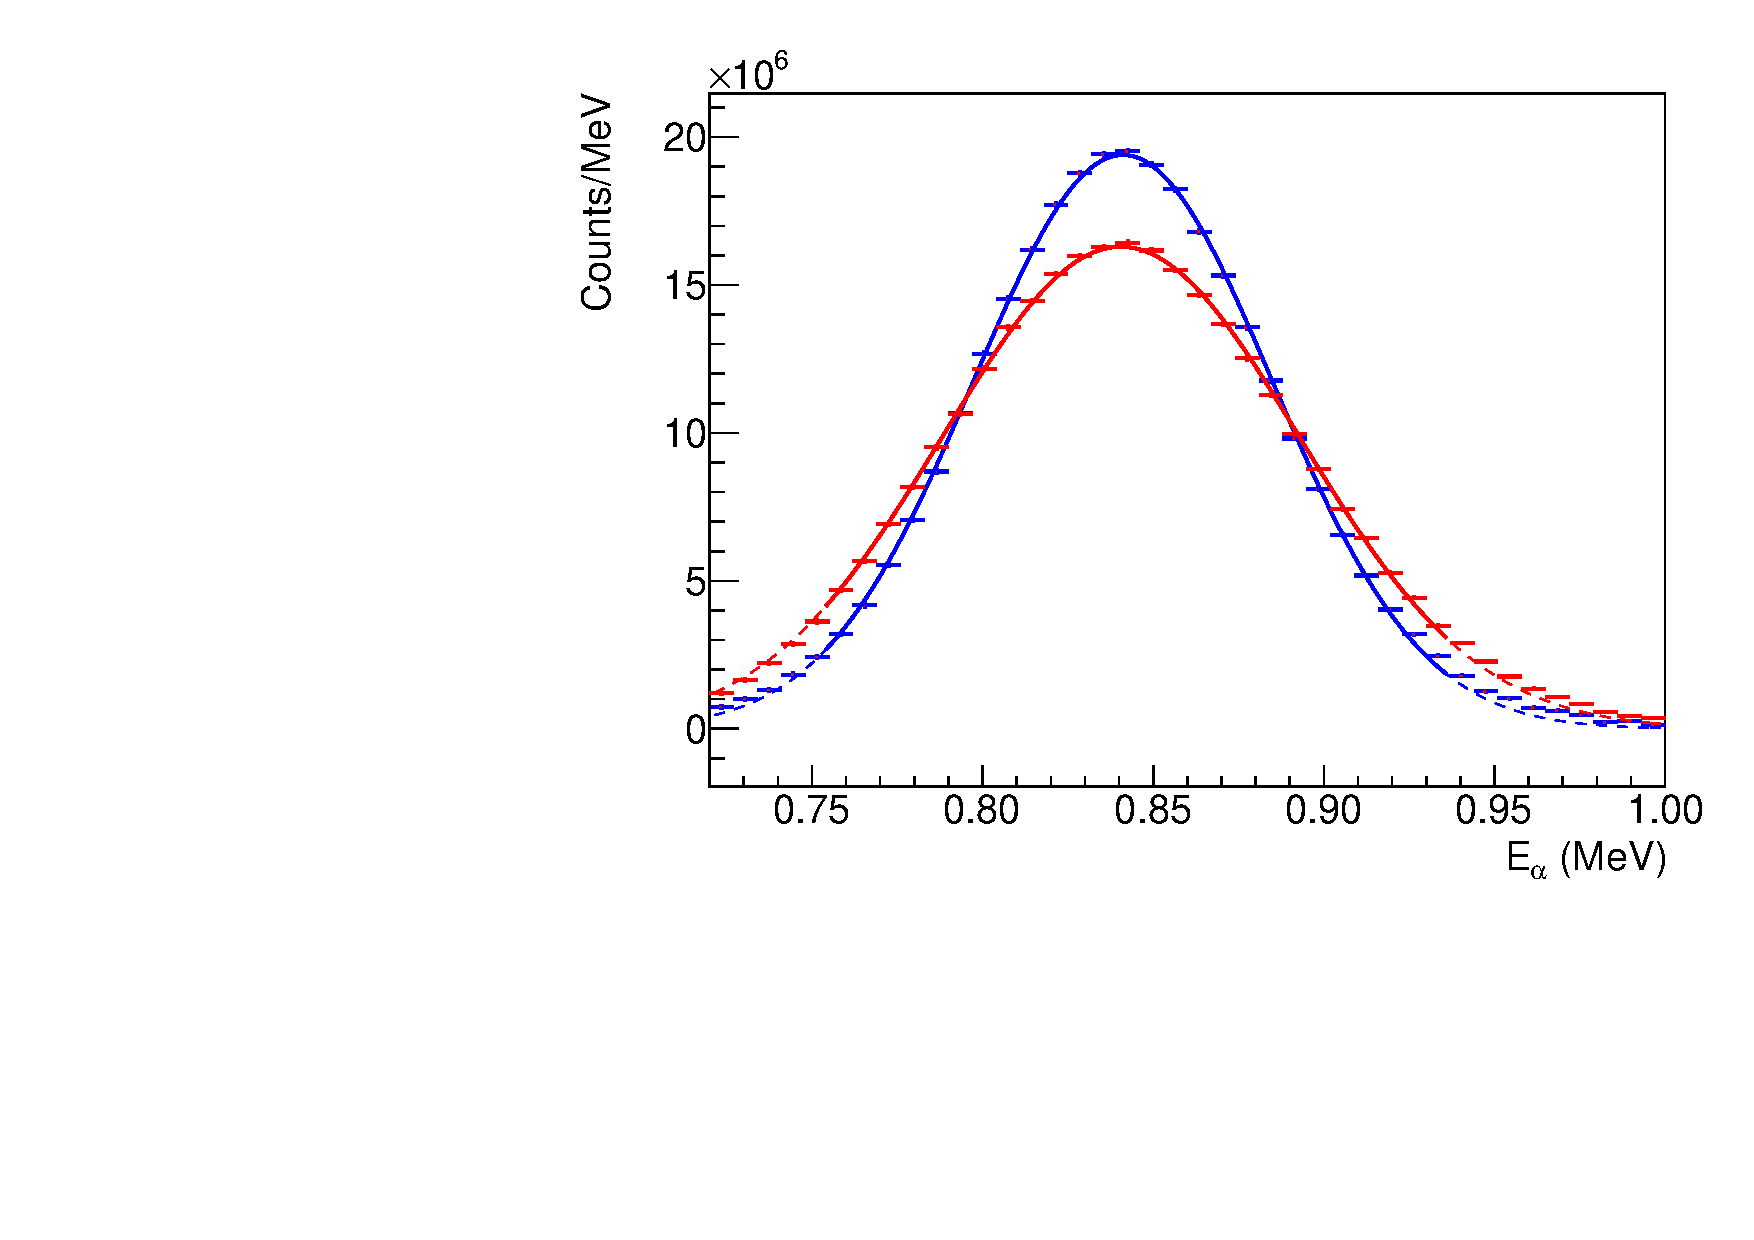
\includegraphics[width=0.56\textwidth]{figures/PubBiPo214AlphaE.pdf}
\caption{\label{fig:AlphaE214}Whole detector Po-214 alpha energy spectrum (blue) and the smeared alpha energy (red). The mean of the unsmeared fit is 0.84454$\pm$0.00009~MeV and the width is 0.04339$\pm$0.00009~MeV.  The solid line shows the fit over the range of data included while the dashed line shows what the fit function looks like in the tails outside the fit region. This is an essentially mono-energetic alpha with 7.687~MeV of energy.}
\end{figure}
\clearpage
\newpage
%------------------------------
\subsection{Whole detector beta energy spectrum}
\begin{figure}[!h]
\centering
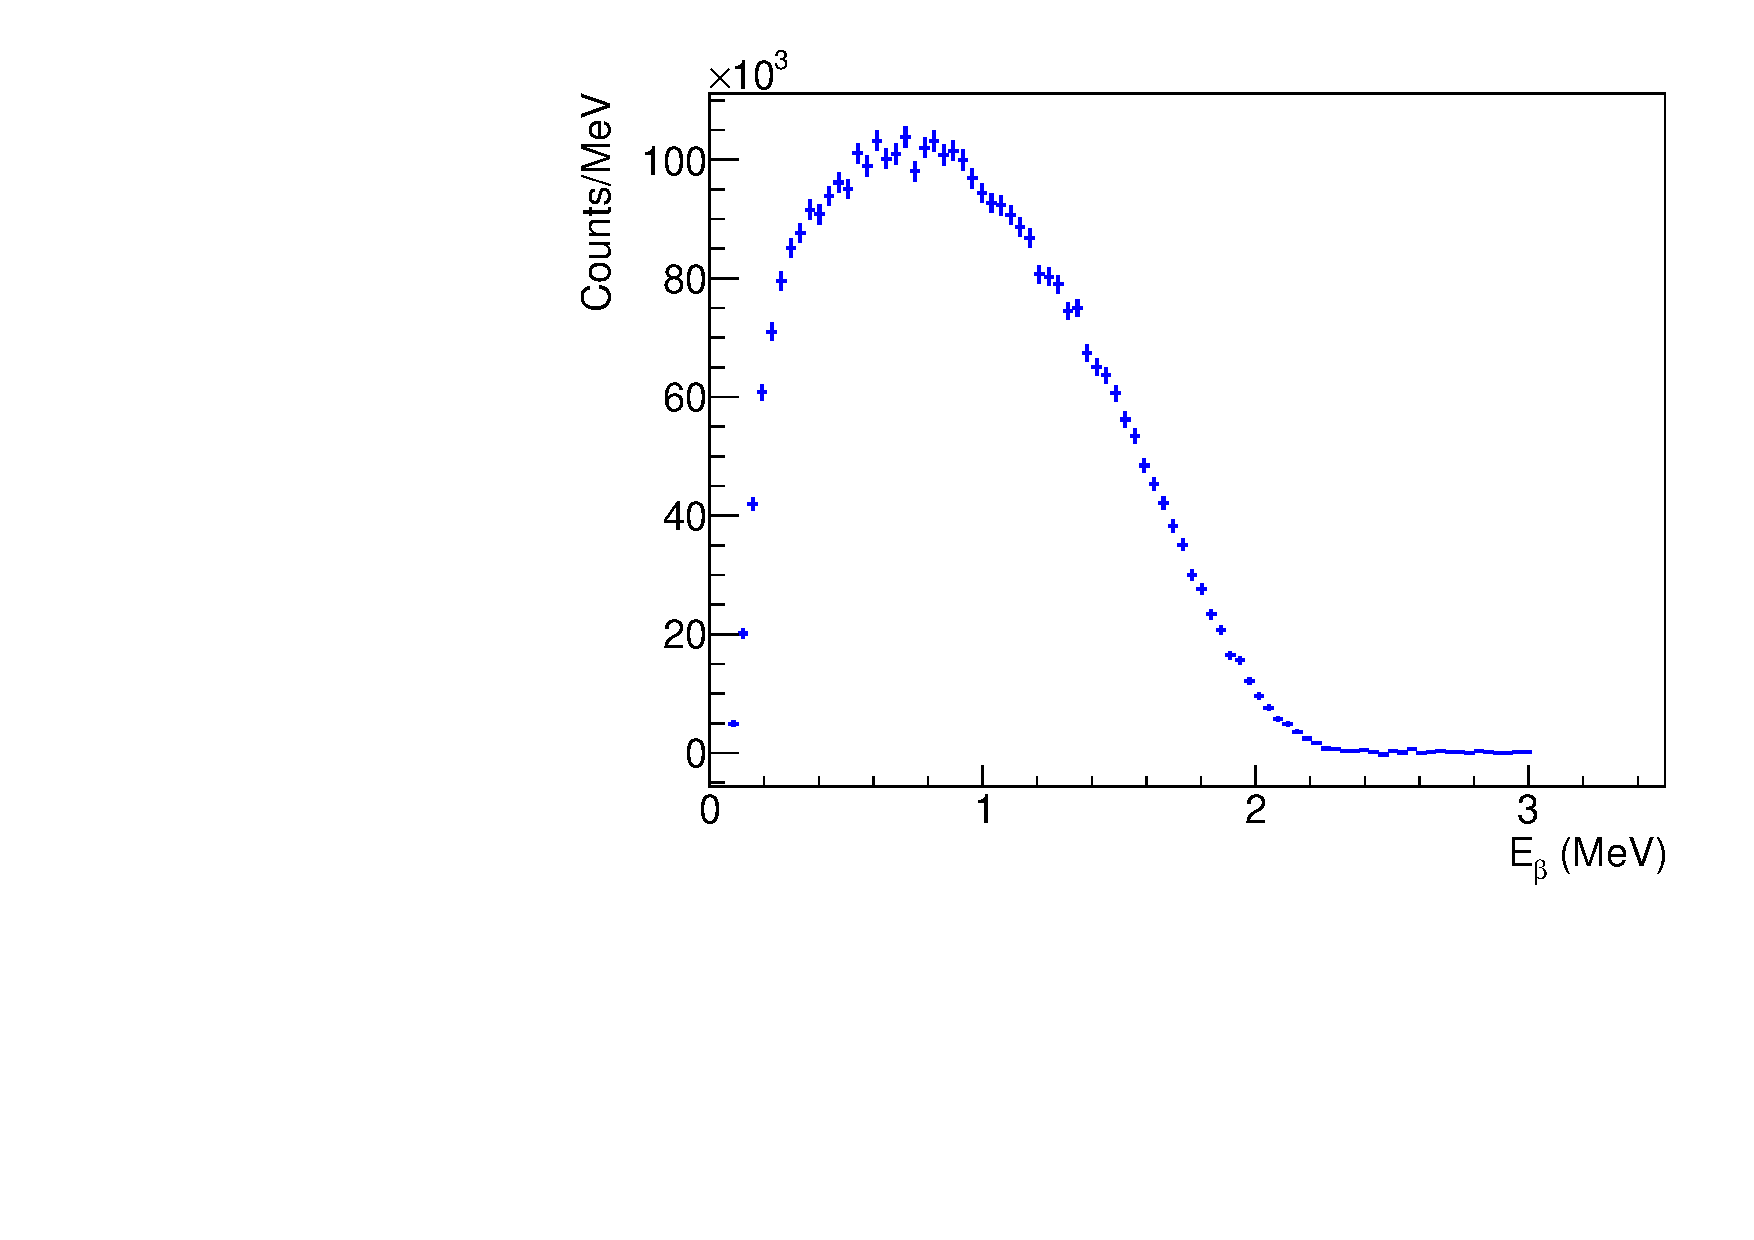
\includegraphics[width=0.7\textwidth]{figures/PubBiPo212BetaE.pdf}
\caption{\label{fig:BetaE212}Whole detector Bi-212 beta energy spectrum. The beta endpoint for this decay is 2.252(2)~MeV.}
\end{figure}
\begin{figure}[!h]
\centering
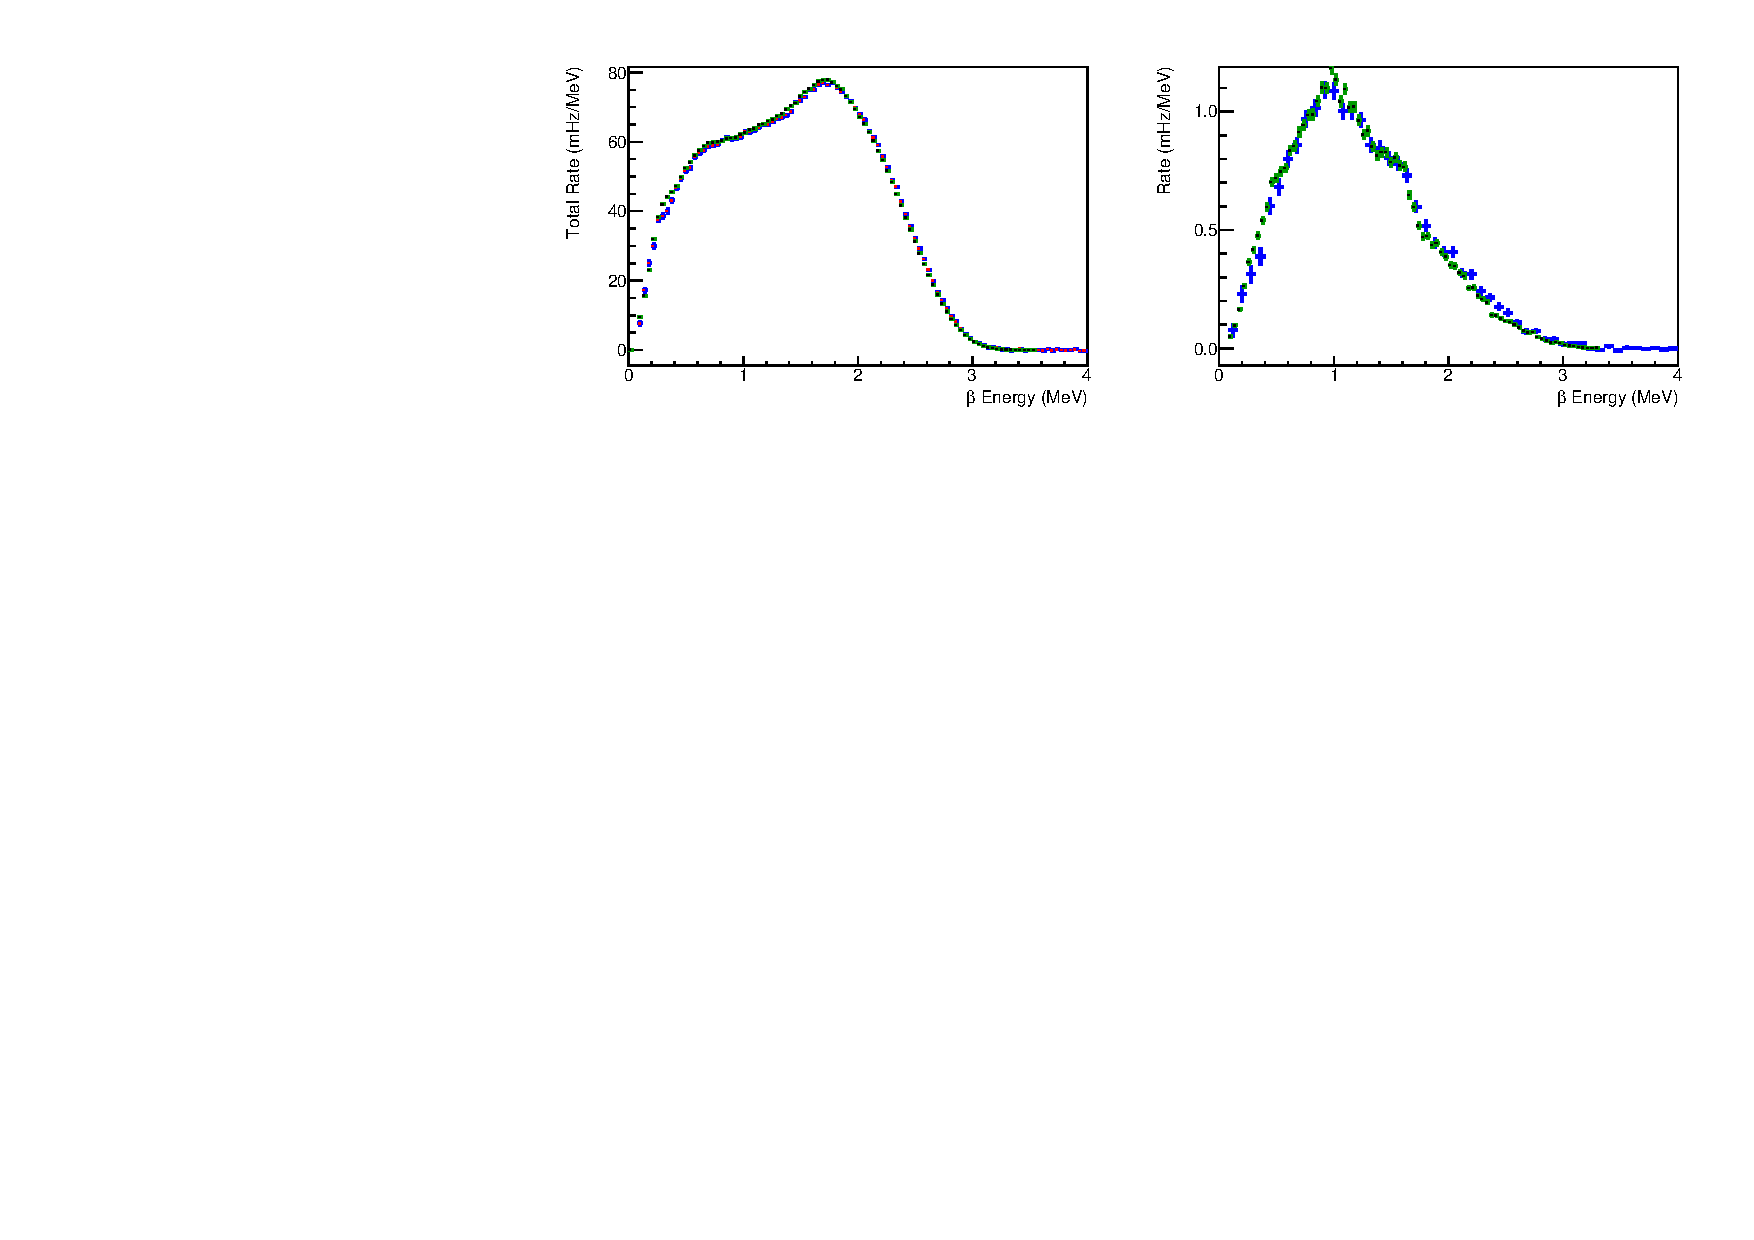
\includegraphics[width=1.0\textwidth]{figures/PubBi214BetaEsimCompare.pdf}
\caption{\label{fig:BetaE214}(Left)Whole detector Bi-214 beta energy spectrum from data (blue) compared to simulation (green). The beta endpoint for this decay is 3.269(11)~MeV. (Right)Segment 76 single cell B-214 beta energy spectrum from data (blue) compared to simulation (green).}
\end{figure}

\clearpage
\newpage
%------------------------------
\subsection{Whole detector Po alpha Z-position distribution}
\begin{figure}[!h]
\centering
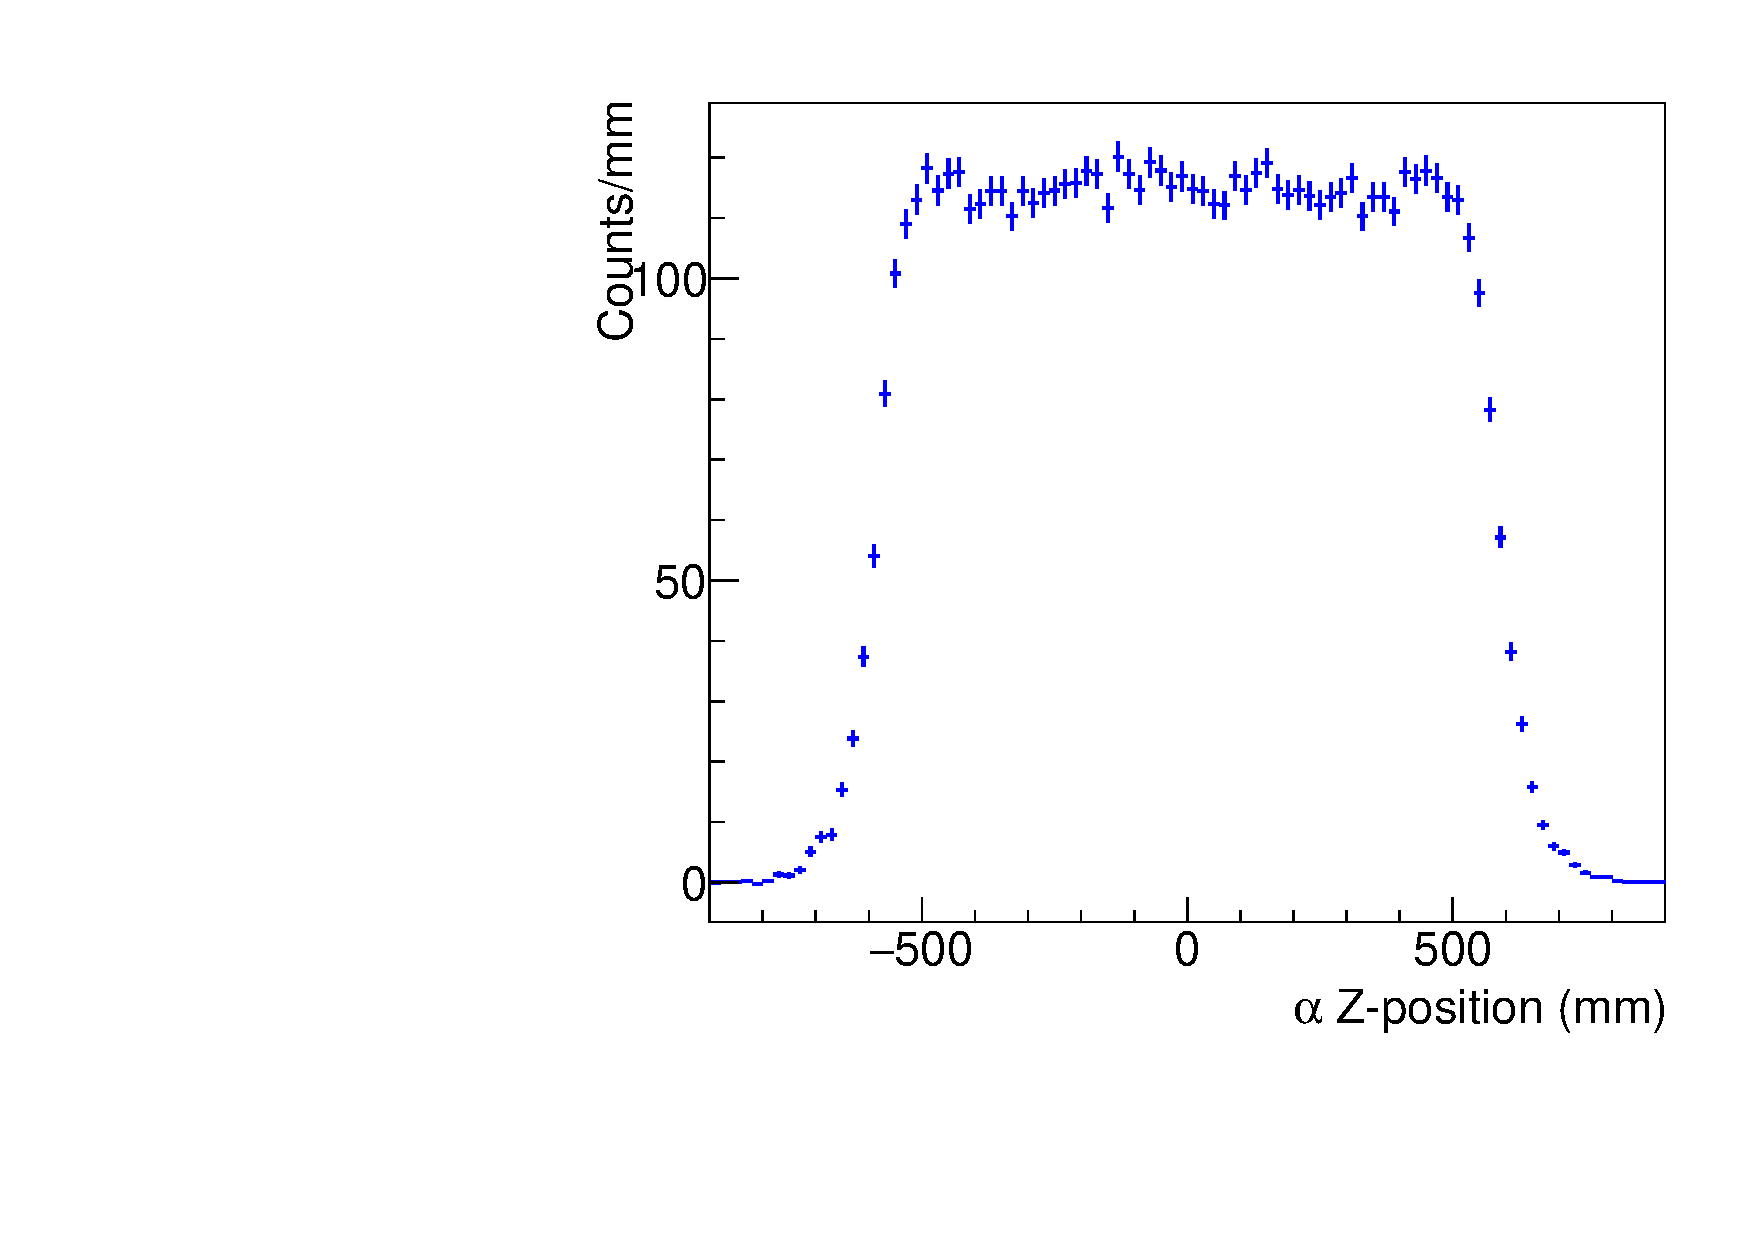
\includegraphics[width=0.6\textwidth]{figures/PubBiPo212Zdistribution.pdf}
\caption{\label{fig:Z212}Whole detector Po-212 alpha Z-position distribution.}
\end{figure}
\begin{figure}[!h]
\centering
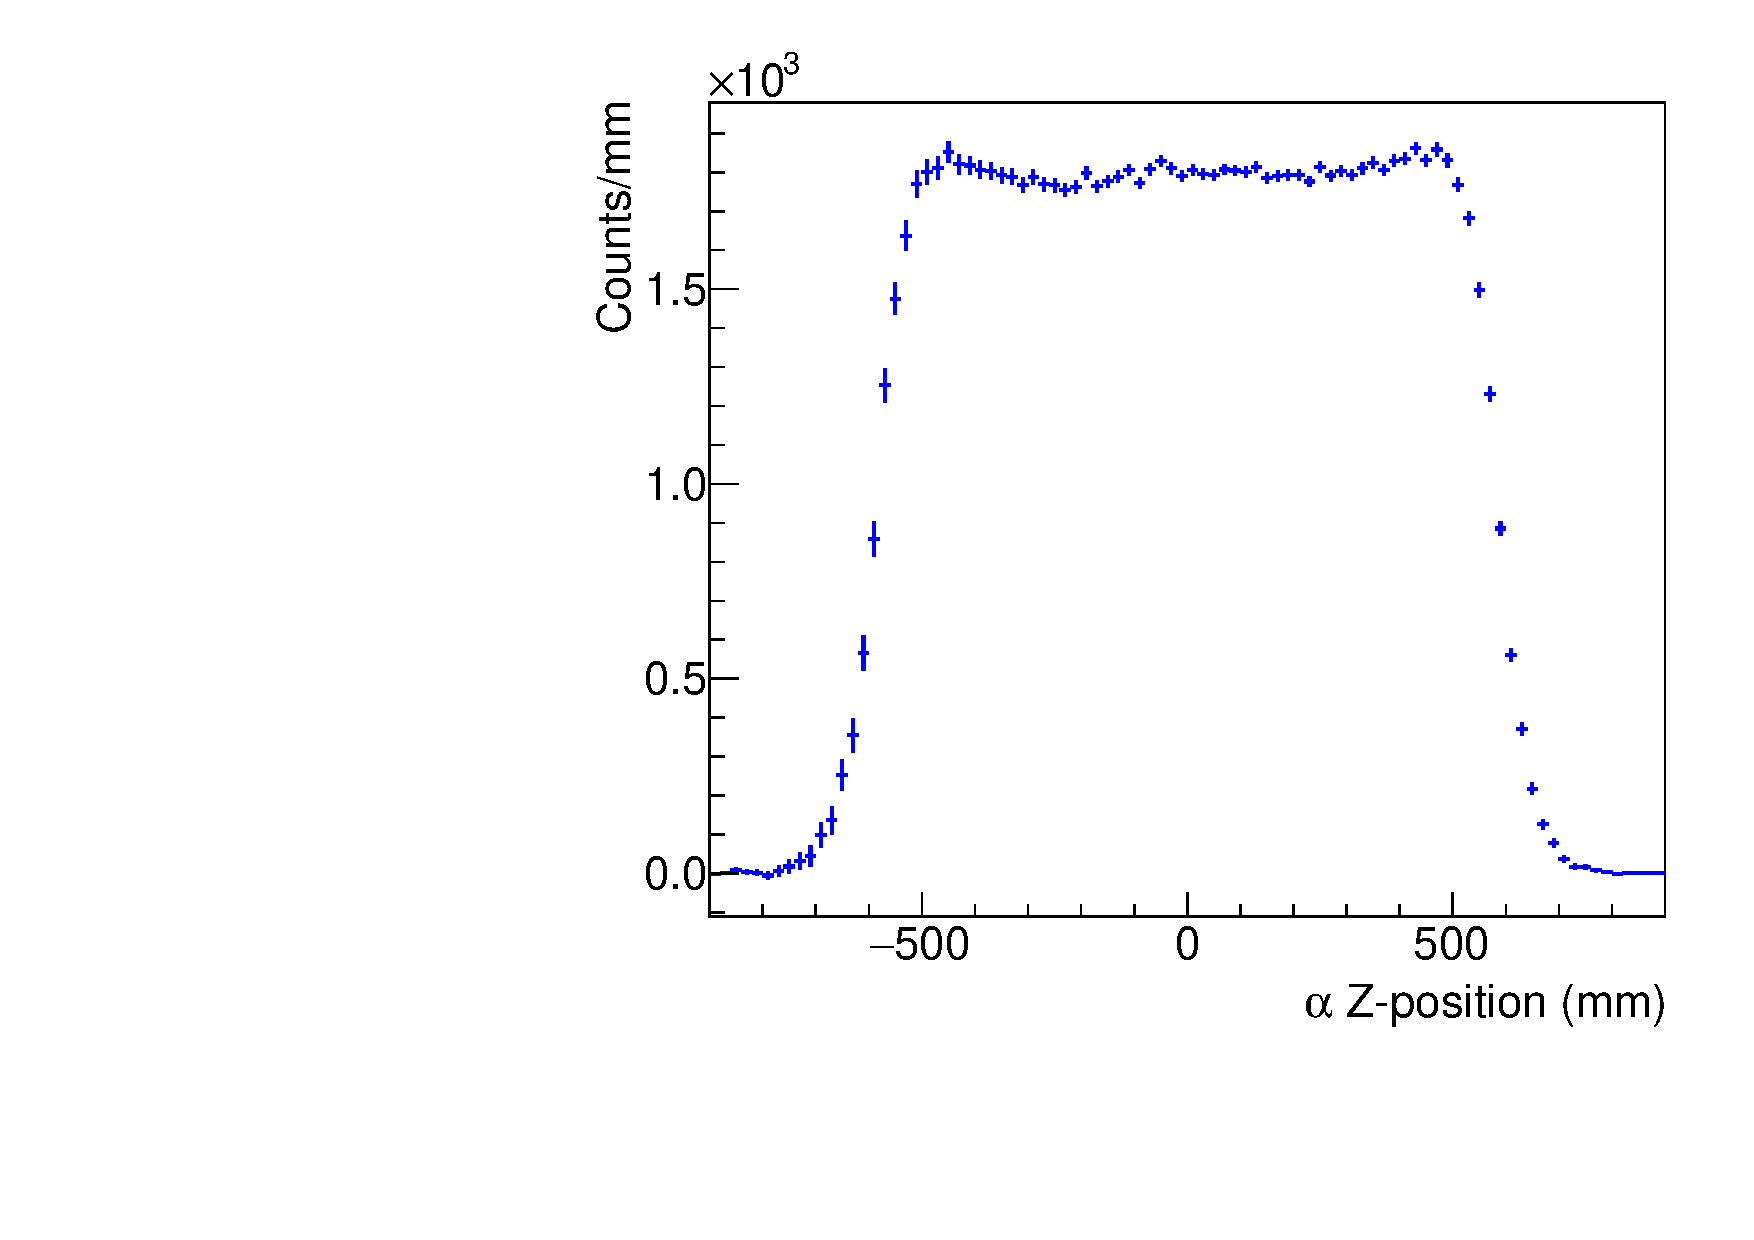
\includegraphics[width=0.6\textwidth]{figures/PubBiPo214Zdistribution.pdf}
\caption{\label{fig:Z214}Whole detector Po-214 alpha Z-position distribution.}
\end{figure}
\newpage
%------------------------------
\subsection{Whole detector BiPo dZ distribution}
\begin{figure}[!h]
\centering
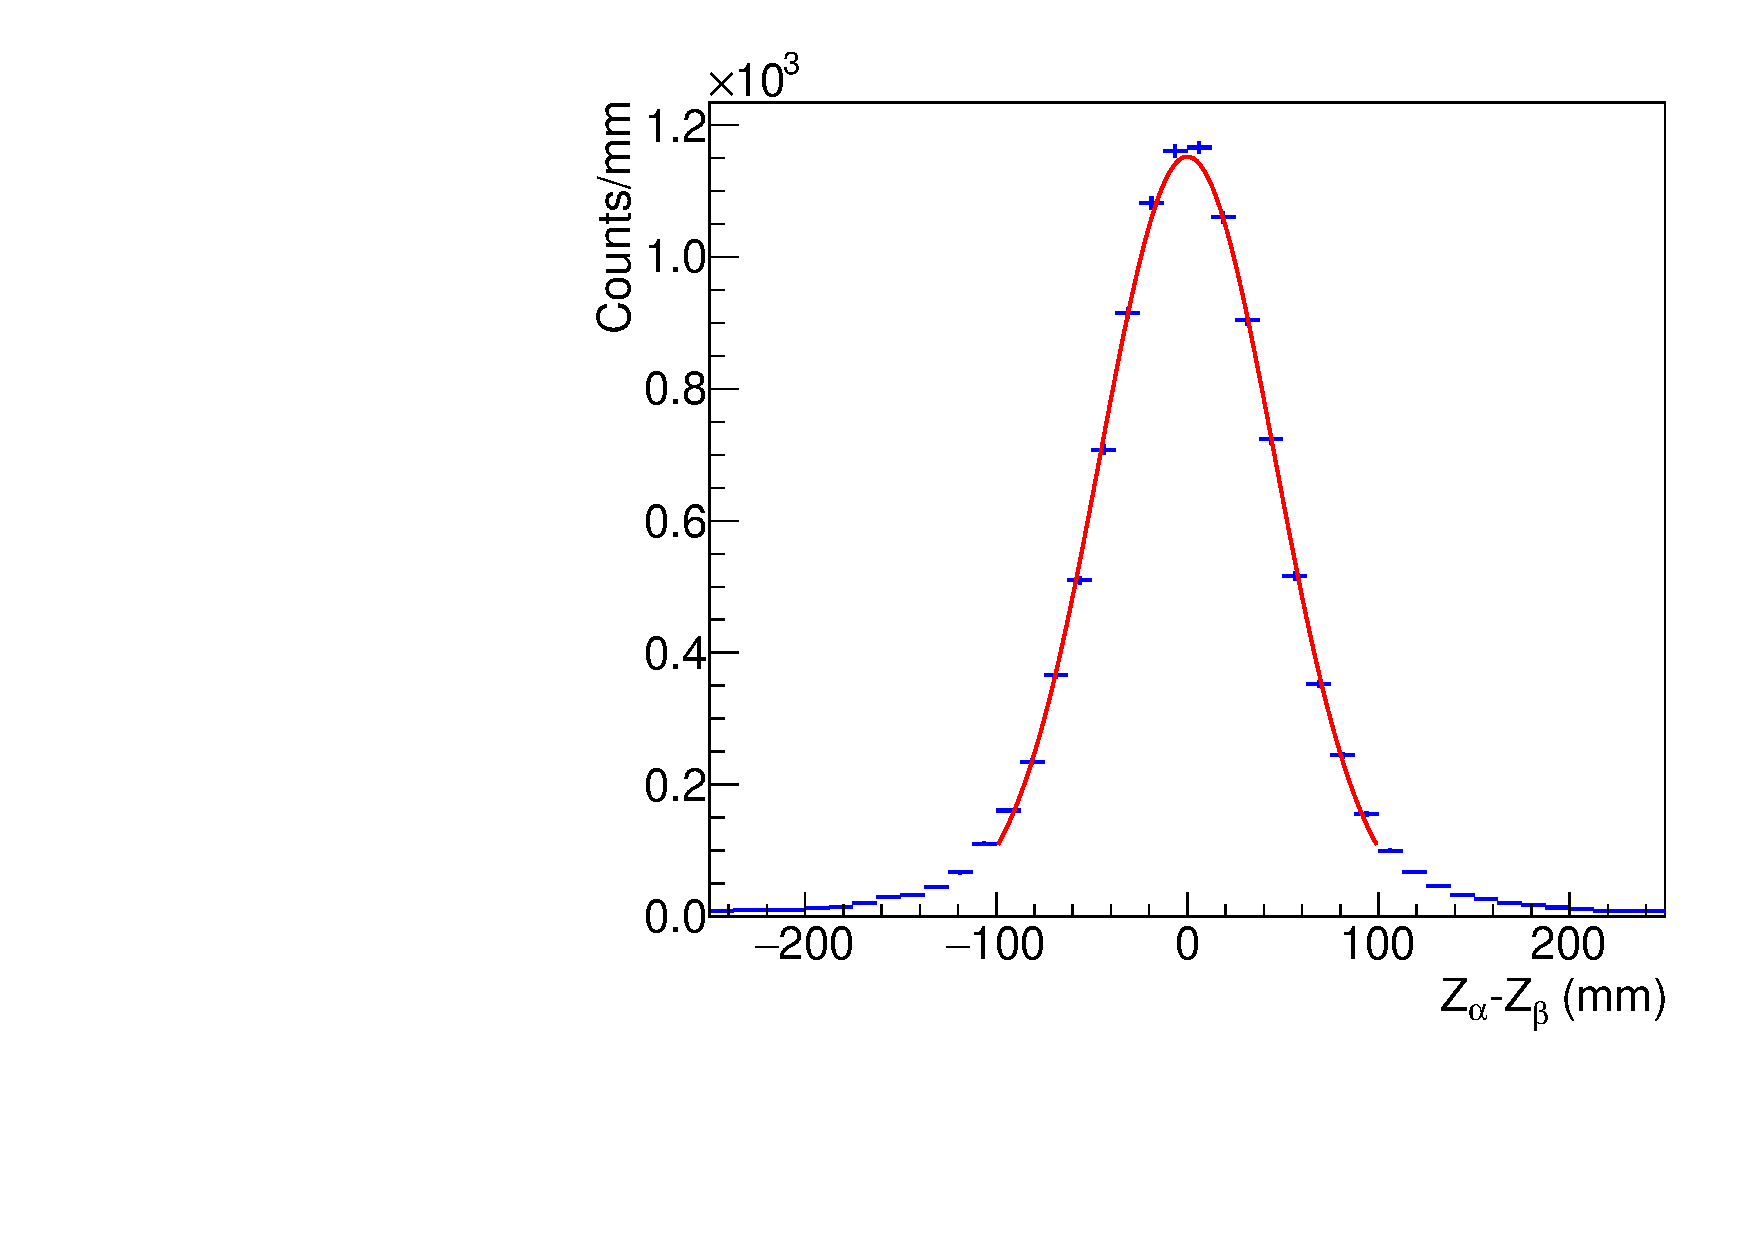
\includegraphics[width=0.55\textwidth]{figures/PubBiPo212dZ.pdf}
\caption{\label{fig:dZ212}Whole detector distribution of Po-212 alpha, beta correlation distance $\Delta$Z. The width of this distribution is 46.06$\pm$0.13~mm.}
\end{figure}
\begin{figure}[!h]
\centering
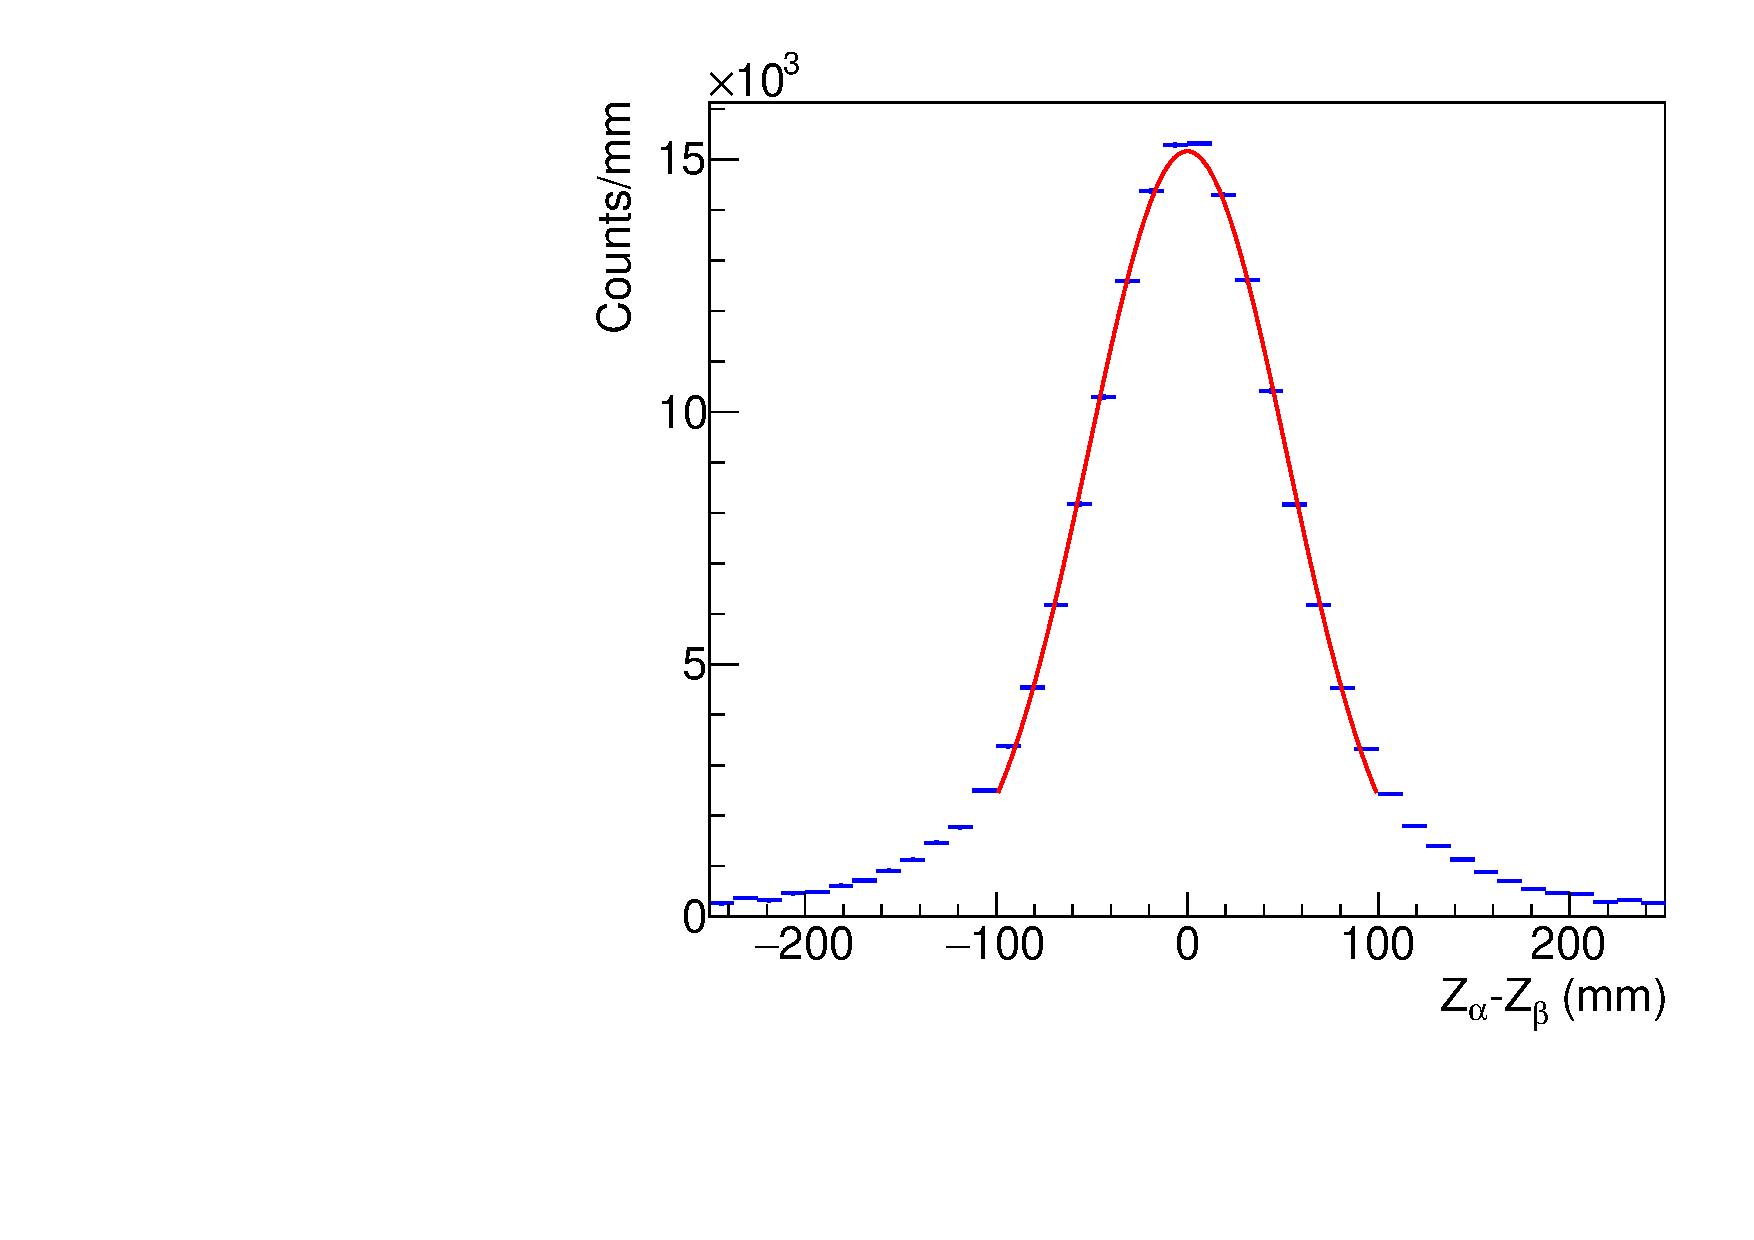
\includegraphics[width=0.55\textwidth]{figures/PubBiPo214dZ.pdf}
\caption{\label{fig:dZ214}Whole detector distribution of Po-214 alpha, beta correlation distance $\Delta$Z. The width of this distribution is 52.85$\pm$0.19~mm. The increase in width is likely due to the higher energy gammas in this decay.}
\end{figure}
\newpage

\FloatBarrier

\section{Supplementary plots\label{sec:supp}}

This section contains supplementary plots that help explain/visualize the analysis process but which are not being submitted for official review for use in publication materials.
Figure \ref{fig:BetaE214} compares simulation and data for the Bi-214 beta spectrum. These appear to have an offset. Figure \ref{fig:BetaE214res} shows the whole detector Bi-214 beta energy spectrum from data (blue) compared to simulation (green) with an energy scale factor of 1.0072 applied to the simulation. This scale factor was found by minimizing the $\chi^2$ goodness of fit between the simulation and the data. The 0.4\% assigned uncertainty in our energy scale combined with the 0.34\%  uncertainty in the beta endpoint could easily explain this discrepancy.   Figure \ref{ig:BetaE214Chisq} shows a plot of the $\chi^2$ parameter over a range of phase space of the scale factor and a spectrum normalization factor. The $\chi^2$ was only calculated using the energy range above 0.4~MeV to avoid obvious low energy deviations. Although the endpoint of the spectrum is 3.27~MeV, the energy range all the way to 4~MeV was included since it had negligible impact on the result.   
\begin{figure}[!h]%use SimComp.C to create plot
	\centering
	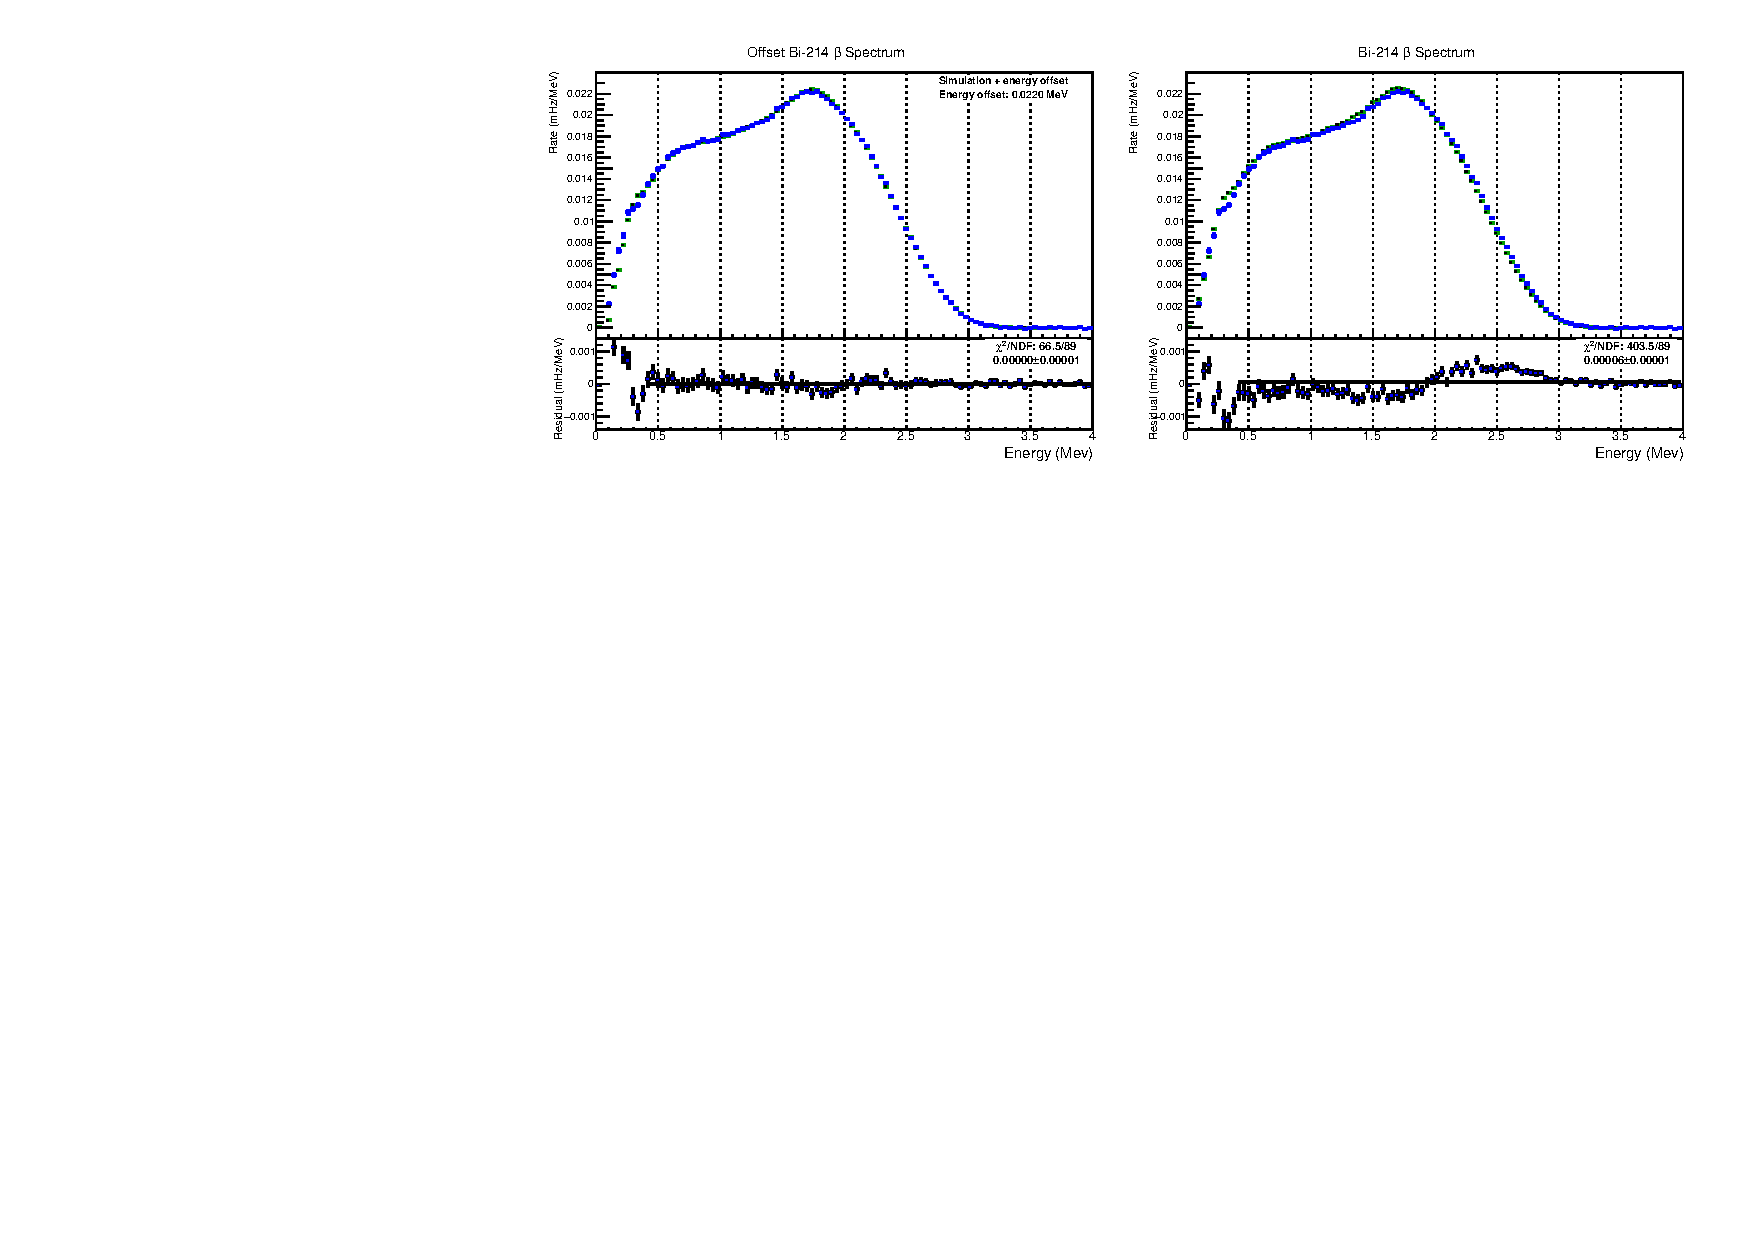
\includegraphics[width=1.0\textwidth]{figures/Bi214BetaSpectrumDataMC.pdf}
	\caption{\label{fig:BetaE214res}(Left)Whole detector Bi-214 beta energy spectrum from data (blue) compared to simulation (green) with an energy scale factor of 1.0072(40) (where the error is the approximate energy shift that introduces a unit shift in $\chi^2$) applied to the simulation providing a nice match. The beta endpoint for this decay is 3.269(11)~MeV. (Right)Whole detector Bi-214 beta energy spectrum from data (blue) compared to simulation (green) with NO energy scaling applied. A constant fit is shown to the residuals in the bottom panels.}
\end{figure}
\begin{figure}[!h]%use SimComp.C to create plot
	\centering
	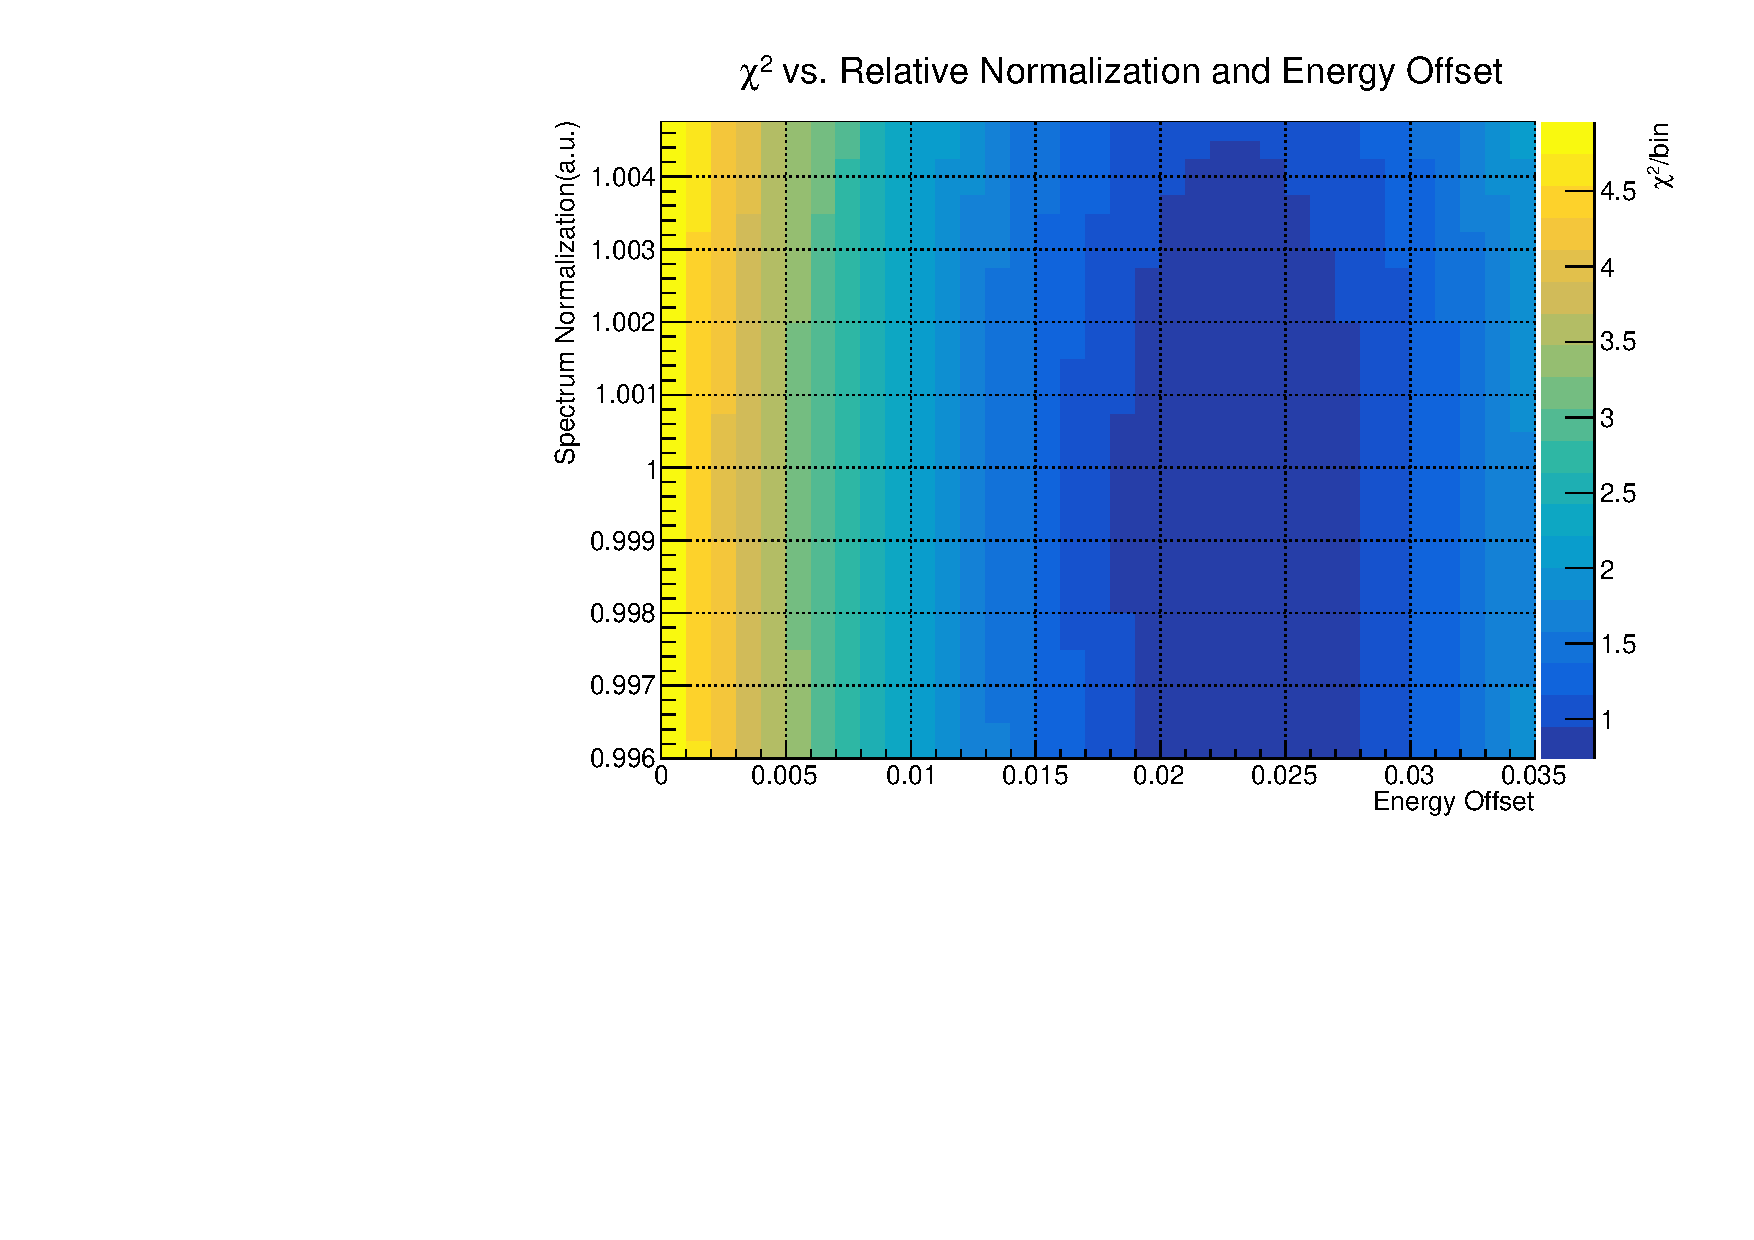
\includegraphics[width=0.68\textwidth]{figures/Bi214BetaSpectrumChisq.pdf}
	\caption{\label{fig:BetaE214Chisq}$\chi^2$/bin shown for varying spectrum normalization and energy scaling. The $\chi^2$ calculation was limited to bins in the energy range from 0.4-4.0~MeV.}
\end{figure}


\begin{figure}[!h]
\centering
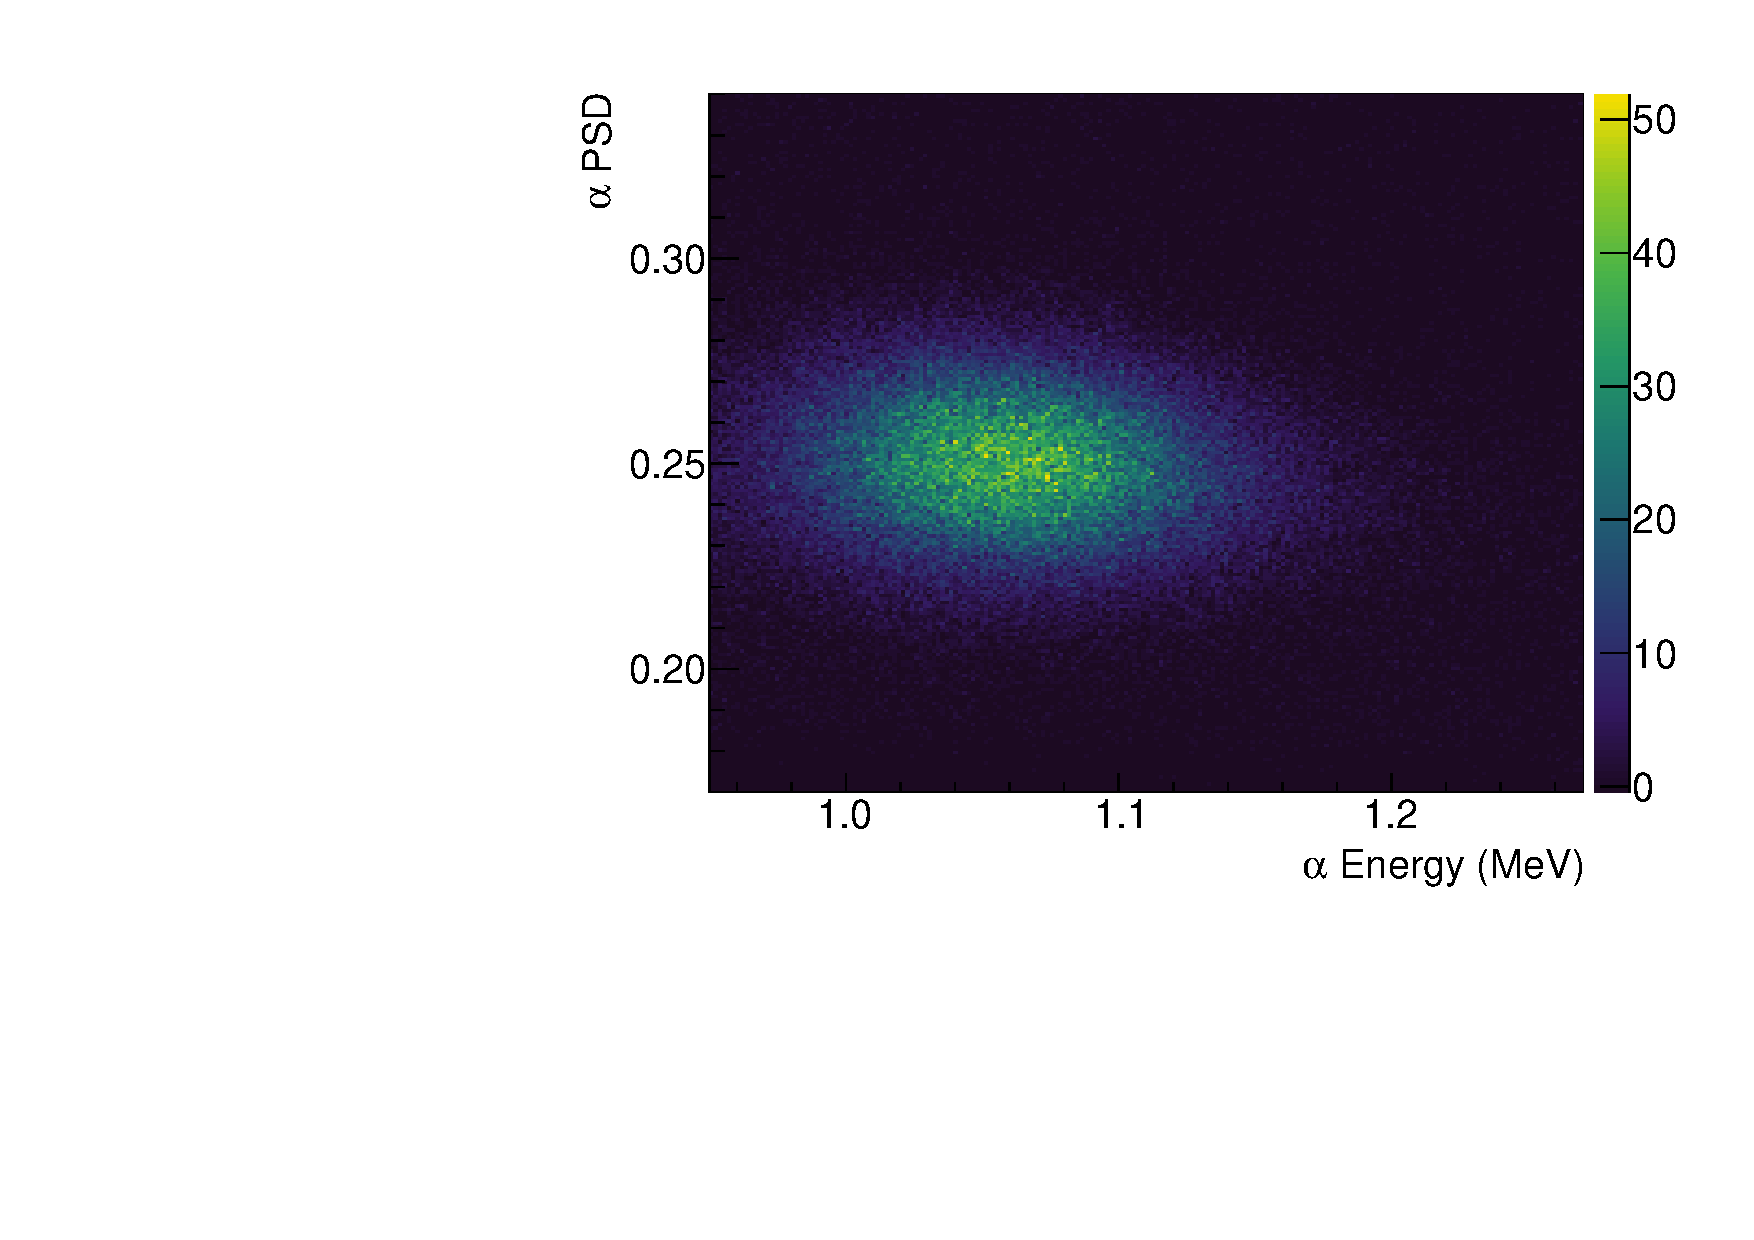
\includegraphics[width=0.7\textwidth]{figures/BiPo212AlphaPSDvsE.pdf}
\caption{\label{fig:apsd212}Po-212 alpha PSD vs energy selection.}
\end{figure}
\begin{figure}[!h]
\centering
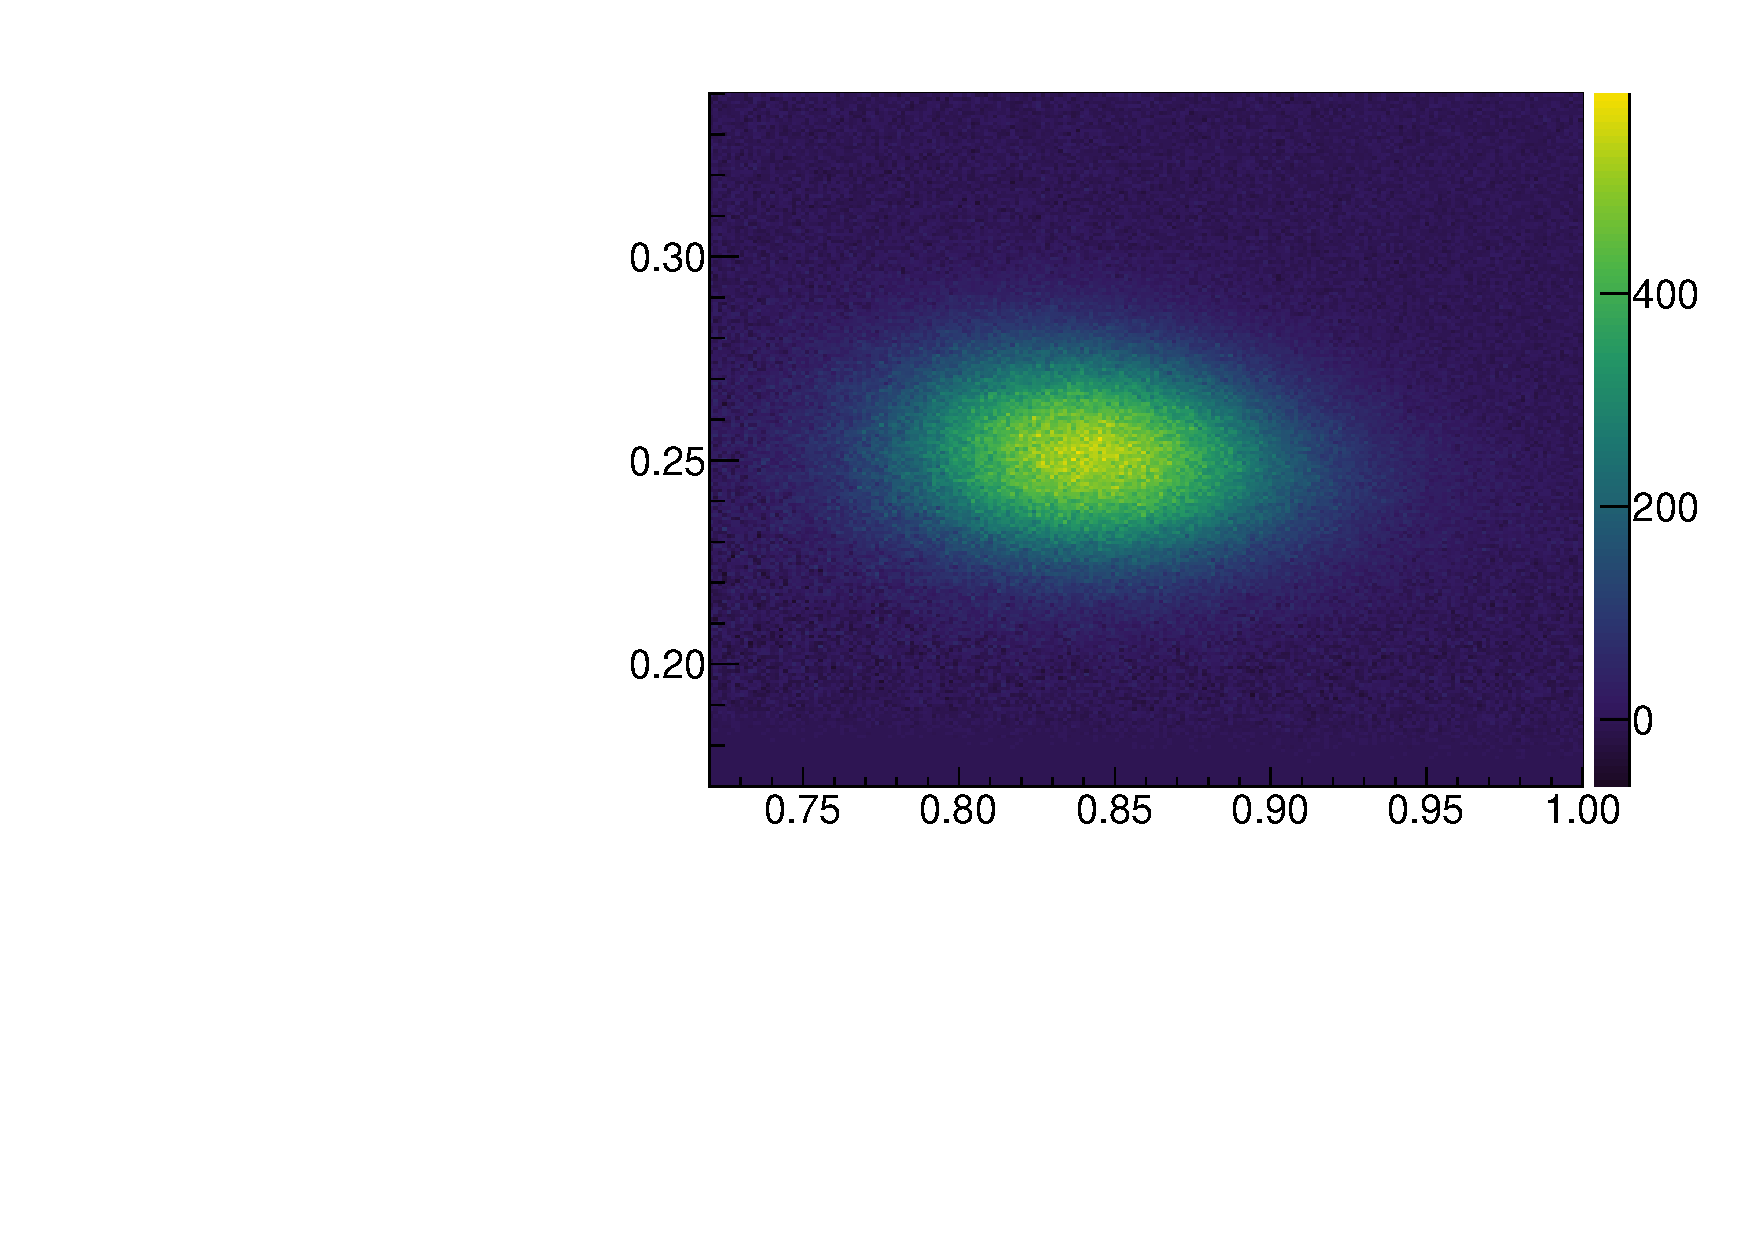
\includegraphics[width=0.7\textwidth]{figures/BiPo214AlphaPSDvsE.pdf}
\caption{\label{fig:apsd214}Po-214 alpha PSD vs energy selection.}
\end{figure}
\begin{figure}[!b]
\centering
\includegraphics[width=0.7\textwidth]{figures/BiPo212BetaPSDvsE.pdf}
\caption{\label{fig:bpsd212}Po-212 beta PSD vs energy selection. The beta PSD shown here is for the first event in each prompt cluster.}
\end{figure}
\begin{figure}[!b]
\centering
\includegraphics[width=0.7\textwidth]{figures/BiPo214BetaPSDvsE.pdf}
\caption{\label{fig:bpsd214}Po-214 beta PSD vs energy selection. The beta PSD shown here is for the first event in each prompt cluster.}
\end{figure}
\begin{figure}[!b]
\centering
\includegraphics[width=0.7\textwidth]{figures/BiPo212DeltaTSpectrum.pdf}
\caption{\label{fig:dt212}Alpha minus beta time distribution used in Bi-212/Po-212 decay chain analysis. }
\end{figure}

\begin{figure}[!bp]
%\begin{minipage}[b]{0.48\textwidth}
\centering
\includegraphics[width=0.7\textwidth]{figures/BiPo214DeltaTSpectrum.pdf}
\caption{\label{fig:dt214}Alpha minus beta time distribution used in Bi-214/Po-214 decay chain analysis.}
\end{figure}
\clearpage
\newpage

\begin{figure}[!bp]
	%\begin{minipage}[b]{0.48\textwidth}
	\centering
	\includegraphics[width=0.8\textwidth]{figures/BiPo1HeatMap.pdf}
	\caption{\label{fig:bipo212heatmap}BiPo-212 event rate by segment map.}
\end{figure}

\begin{figure}[!bp]
	%\begin{minipage}[b]{0.48\textwidth}
	\centering
	\includegraphics[width=0.8\textwidth]{figures/BiPo0HeatMap.pdf}
	\caption{\label{fig:bipo214heatmap}BiPo-214 event rate by segment map.}
\end{figure}
\clearpage
\newpage

\section{Supporting Documentation}

\subsection{Links to any past DocDB entries related to the plot:} 
\hspace{2in}
%\bibliography{}
\bibliography{citations.bib}{}

\end{document}
